% ------------------------------------------------------------------------
%
% -------------------      Plantilla_UIS.tex       -----------------------
%
% ------------------------------------------------------------------------
% ------------------------------------------------------------------------
% ------------------------------------------------------------------------
% Versi�n de plantilla para realizaci�n de informes de trabajo de grado
% construida para uso de la Universidad Industrial de Santander.
%
% Reservados todos los derechos
%
% Bucaramanga, Colombia
%
% Febrero 03 de 2019
%
% ------------------------------------------------------------------------
% ------------------------------------------------------------------------
% ------------------------------------------------------------------------
%
% ------------------------------------------------------------------------
\documentclass[letter,oneside,12pt,spanish]{report}          % Encabezados
% ------------------------------------------------------------------------
\usepackage{uislatexstyleAPA}                           % Libreria UIS APA
% ------------------------------------------------------------------------
% Ingrese en este punto las librer�as espec�ficas de usuario
% ------------------------------------------------------------------------
\usepackage{epsfig}
\usepackage{amsmath}
\usepackage{amssymb}
\usepackage{subfigure}
\usepackage{hyperref}
% ------------------------------------------------------------------------
\begin{document}                                     % Inicio de documento
% ------------------------------------------------------------------------
% Definici�n sil�bica de palabras
% ------------------------------------------------------------------------
\hyphenation{pro-por-cio-nal di-se-�o}
\hypersetup {pdfborder = {0 0 0}}
% ------------------------------------------------------------------------
% Titulo resumido del trabajo que aparecer� en cornisa
% ------------------------------------------------------------------------
\title{CONJUNTOS ESTABILIZANTES EN CONTROLADORES PI}
% ------------------------------------------------------------------------
% Elementos previos al contenido del trabajo
% ------------------------------------------------------------------------
% ------------------------------------------------------------------------
%                               Portadilla
% ------------------------------------------------------------------------

\begin{center}

Verificaci�n de Conjuntos Estabilizantes para el M�todo de Dise�o de Controladores PI de Ziegler \& Nichols \vspace{2.3cm}

Emerson Rey Ardila\\ \vspace{2.3cm}

Trabajo de Grado para optar al t�tulo de Ingeniero Electr�nico\\ \vspace{2.3cm}

Director\\
Ricardo Alzate Casta�o\\
Doctorado en Ingenier�a Inform�tica y Autom�tica \vspace{2.4cm}

Universidad Industrial de Santander\\
Facultad de Ingenier�as Fisicomec�nicas\\
Escuela de Ingenier�as El�ctrica, Electr�nica y de Telecomunicaciones\\
Bucaramanga\\
2019\\

\end{center}

             % Portadilla
% ------------------------------------------------------------------------
% ------------------------------------------------------------------------
% ------------------------------------------------------------------------
% ------------------------------------------------------------------------
%                               Dedicatoria
% ------------------------------------------------------------------------
% ------------------------------------------------------------------------
% ------------------------------------------------------------------------
\chapter*{Dedicatoria}

\noindent Este trabajo viene dedicado para todas aquellas personas que apoyaron el desarrollo
y ejecuci�n de este trabajo de grado.\\

En especial reconozco la permanente presencia de Dios en mi camino de vida.
% ------------------------------------------------------------------------                                    % Dedicatoria
% ------------------------------------------------------------------------
\begin{center}
    \textbf{Agradecimientos}
\end{center}


%% Aquí van los agradecimientos

Al bicho siuuu



\newpage                               % Agradecimientos
% ------------------------------------------------------------------------
\tableofcontents                                      % Tabla de contenido
% ------------------------------------------------------------------------
\listoffigures                         % Lista de figuras, tablas y anexos
\listoftables
\listofanexo
% ------------------------------------------------------------------------
% ------------------------------------------------------------------------
% ------------------------------------------------------------------------
% ------------------------------------------------------------------------
%                                Glosario
% ------------------------------------------------------------------------
% ------------------------------------------------------------------------
% ------------------------------------------------------------------------
\chapter*{Glosario}

\begin{description}
  \item[Controlador] (o tambi�n compensador) es un dispositivo que toma una decisi�n con base en la comparaci�n de la informaci�n
  medida con respecto a condiciones deseadas de operaci�n. A dicha decisi�n se le denomina acci�n de control.
  \item[Controlar] es asignar valores a la variable manipulada para lograr que la variable controlada siga un valor de referencia.
  \item[Perturbaci�n] se�al indeseada que afecta negativamente el valor de la variable controlada del sistema.
  \item[PID] sigla que refiere la acci�n combinada de control proporcional, integral y derivativo.
  \item[Sistema] conjunto de elementos que interact�an de manera organizada para cumplir con un fin u objetivo com�n.
  \item[Variable Controlada] es la cantidad o condici�n que se mide y controla.
  \item[Variable Manipulada] es la cantidad que el controlador modifica para afectar los valores de salida de la planta.
\end{description}
% ------------------------------------------------------------------------                              % Glosario de t�rminos
% ------------------------------------------------------------------------
% Contenido del Informe
% ------------------------------------------------------------------------
% ------------------------------------------------------------------------
% ------------------------------------------------------------------------
% ------------------------------------------------------------------------
%                                Resumen
% ------------------------------------------------------------------------
% ------------------------------------------------------------------------
% ------------------------------------------------------------------------
\chapter*{Resumen}

\footnotesize{
\begin{description}
  \item[T�tulo:] Verificaci�n de Conjuntos Estabilizantes para Dise�o de Controladores PI de Ziegler \& Nichols \astfootnote{Trabajo de grado}
  \item[Autor:] Emerson Rey Ardila \asttfootnote{Facultad de Ingenier�as F�sico-Mec�nicas. Escuela de Ingenier�as El�ctrica, Electr�nica y telecomunicaciones. Director: Ricardo Alzate Casta�o, Doctorado en Ingenier�a Inform�tica y Autom�tica.}
  \item[Palabras Clave:] Conjunto Estabilizante, Controladores PI, Dise�o Gr�fico de Compensadores, M�todo de Ziegler \& Nichols.
  \item[Descripci�n:] El presente proyecto presenta el c�lculo de conjuntos estabilizantes para sistemas SISO LTI controlados por compensadores de estructura simple. Se estudia la fragilidad de controladores PI calculados empleando el m�todo \emph{Ziegler \& Nichols}, t�cnica de referencia en m�ltiples aplicaciones de ambito industrial. A partir de la definici�n para una m�trica basada en la interpretaci�n geom�trica para los m�rgenes de estabilidad del sistema controlado, se verifica que el controlador dise�ado con el m�todo en cuesti�n no necesariamente tolera variaciones significativas en sus valores de par�metro. Por el contrario, asume comportamientos cercanos a los l�mites de estabilidad proporcionados mediante el c�lculo de su conjunto estabilizante. Lo anterior se convierte en informaci�n importante tomando en cuenta que generalmente los m�todos de dise�o se someten a un ajuste fino. Como m�trica, se define el espacio planar correspondiente con la intersecci�n entre una elipse y una l�nea recta que representan lugares geom�tricos de m�rgen de fase y/o ganancia constantes. Adicional a lo anterior, se desarroll� una interfaz en MATLAB que permite calcular gr�ficamente los par�metros del controlador a partir de un conjunto admisible de especificaciones con base en su conjunto estabilizante. Trabajo complementario incluye la utilizaci�n de t�cnicas computacionales para el c�lculo de
conjuntos estabilizantes sobre plantas arbitrarias.
\end{description}}\normalsize
% ------------------------------------------------------------------------                                                % Resumen
% ------------------------------------------------------------------------
% ------------------------------------------------------------------------
% ------------------------------------------------------------------------
%                                Abstract
% ------------------------------------------------------------------------
% ------------------------------------------------------------------------
% ------------------------------------------------------------------------
\chapter*{Abstract}

\footnotesize{
\begin{description}
  \item[Title:] Stabilizing Set Verification for the Ziegler \& Nichols PI Controller's Design Method\astfootnote{Bachelor Thesis}
  \item[Author:] Emerson Rey Ardila\asttfootnote{Facultad de Ingenier�as F�sico-Mec�nicas. Escuela de Ingenier�as El�ctrica, Electr�nica y telecomunicaciones. Director: Ricardo Alzate Casta�o, Doctorado en Ingenier�a Inform�tica y Autom�tica.}
  \item[Keywords:] Graphical Design of Compensators, PI Controllers, Stabilizing Set, Ziegler \& Nichols Classical Method.
  \item[Description:] In this work the calculation for stabilizing sets of SISO LTI plants controlled by single structure compensators is presented. In particular, the fragility of PI controllers calculated by employing the classical method of \emph{Ziegler \& Nichols} is tested by defining a measure based on geometrical interpretation of margins of stability for the controlled loop. As we already now, the \emph{Ziegler \& Nichols} method is a reference technique for many industrial applications in practice but surprisingly after tuning parameters for desired performance the controlled system sometimes will operate riskily closed to stability boundaries determined after calculation of its corresponding stabilizing set. As a measure of the distance to instability, the intersection sets between an ellipse and a straight line constructed for constant gain and/or phase margin, is proposed. This measure shows that the controller calculated is not tolerant to changes in the parameter values, a situation typical in practice by the so-called fine tuning procedures. Also, a software interface was developed to perform graphical calculation of controller parameters using the achievable specifications set obtained from the stabilizing set of the controlled system. Ongoing work includes the automatic calculation for stabilizing sets in arbitrary plants by using computational tools already developed for that goal.
\end{description}}\normalsize
% ------------------------------------------------------------------------                                               % Abstract
% ------------------------------------------------------------------------
% Cap�tulos
% ------------------------------------------------------------------------
% ------------------------------------------------------------------------
% ------------------------------------------------------------------------
% ------------------------------------------------------------------------
%                              Introducci�n
% ------------------------------------------------------------------------
% ------------------------------------------------------------------------
% ------------------------------------------------------------------------

\nnchapter{Introducci�n}
% ------------------------------------------------------------------------
% ------------------------------------------------------------------------

\noindent Dise�ar un controlador, puede considerarse como el arte de determinar la estructura
y los par�metros de un sistema para modificar a conveniencia el comportamiento
de otro. En este proceso, llevar a la pr�ctica dicha idea formulada en modo simple,
implica satisfacer requerimientos con recursos limitados en general.\\

La teor�a del control, tanto de tipo cl�sico como moderno, ha intentado resolver este
problema de dise�o atendiendo diferentes criterios de desempe�o que incluyen
consideraciones de error, criterios de optimalidad, robustez, incertidumbre y
adaptabilidad.\\

A pesar de los diferentes criterios y puntos de vista que atienden la tarea del dise�o
 de un controlador, siempre ser� necesario cumplir con una premisa b�sica: la
estabilidad del sistema controlado.\\

Bhattacharyya y Keel \citep{Bhatt97} mostraron que a�n las estrategias m�s refinadas
dedise�o de controladores pueden presentar problemas, al no garantizar estabilidad.\\

Estudios complementarios al anterior, incluyen minuciosos trabajos de alta
componente te�rica orientados a formular t�cnicas refinadas para el c�lculo de
controladores de bajo orden, que garanticen no solamente las premisas requeridas
de desempe�o din�mico para el sistema controlado, sino tambi�n el elemento m�s
importante: ``\emph{su estabilidad}''.\\

El conjunto estabilizante, se define por tanto como todos los posibles valores de
par�metro para un controlador, que garantizan las condiciones de estabilidad
absoluta para el sistema \citep{ Alzate2016}. Estas condiciones de estabilidad absoluta son
f�cilmente verificables en sistemas de bajo orden a trav�s de procedimientos
simples como el criterio de \emph{Routh-Hurwitz} \citep{ogata2010}. Sin embargo, cuando el orden del
sistema, o la cantidad de par�metros del controlador aumenta, dichas inecuaciones
constituyen sistemas no lineales de dif�cil soluci�n anal�tica.\ Algunos autores han
 propuesto  soluciones m�s generalizadas para resolver este tipo de problemas,
basadas en el teorema de \emph{Hermite-Bielher} \citep{fernandes2008} \citep{Datta1999} \citep{Bhatt97}.\\

En particular, se han obtenido resultados aplicados sobre plantas t�picas ante
controladores PID, como se referencia en \citep{Elizondo2013} \citep{Oliveira2003} \citep{silva2002}, complementado por an�lisis de
lazos de control bajo la acci�n de retardos en \citep{Farkh2014} \citep{fernandes2008} \citep{Oliveira2003}. Algunas aplicaciones para
el caso de dise�o de controladores sobre convertidores de potencia pueden
encontrarse en \citep{Bhattachar1994} \citep{Datta2000} \citep{Loera2014}.\\

Tomando en cuenta lo anterior, se evidencia la importancia del an�lisis de conjuntos
estabilizantes en el dise�o de un sistema de control para garantizar su operaci�n
ante distintos escenarios que pueden experimentarse en situaciones pr�cticas. Por
tanto, se analizar� un caso de estudio ampliamente empleado como lo es el m�todo
de \emph{Ziegler \& Nichols}, buscando mostrar la relaci�n que tiene su formulaci�n b�sica
(expresiones matem�ticas y m�todos de c�lculo) con los conjuntos estabilizantes
de sus par�metros soluci�n.\\

A partir de la ejecuci�n del presente trabajo de grado, se buscan respuestas ante
interrogantes como los siguientes: �C�mo se relacionan los par�metros de un
controlador PI calculado por el m�todo de \emph{Ziegler \& Nichols} con su conjunto
estabilizante? �Qu� tan propensa al estado de inestabilidad es una planta
controlada a partir del an�lisis anterior? �Demuestra el m�todo de \emph{Ziegler \& Nichols}
sensibilidad ante cambios de par�metro del sistema? �Es f�cil llevar a la
inestabilidad un sistema controlado mediante un controlador PI dise�ado
empleando el m�todo de \emph{Ziegler \& Nichols}? En otras palabras �Qu� tan fr�gil es el
m�todo para c�lculo de controladores PI de \emph{Ziegler \& Nichols}?
% ------------------------------------------------------------------------
% ------------------------------------------------------------------------    % Introducci�n
% ------------------------------------------------------------------------
% ------------------------------------------------------------------------
% ------------------------------------------------------------------------
%                              Objetivos
% ------------------------------------------------------------------------
% ------------------------------------------------------------------------
% ------------------------------------------------------------------------

\chapter{Objetivos}
% ------------------------------------------------------------------------
% ------------------------------------------------------------------------

\section*{Objetivo general}

\begin{itemize}
   \item[ ] Analizar las condiciones de estabilidad del conjunto de par�metros PI calculados
   empleando el m�todo de dise�o de controladores de Ziegler \& Nichols.
\end{itemize}

\section*{Objetivos espec�ficos}

\begin{itemize}
    \item[ ] Interpretar las tablas de dise�o de par�metros PI de Ziegler \& Nichols en t�rminos de conjuntos estabilizantes;
    \item[ ] Desarrollar un algoritmo que permita verificar las condiciones de estabilidad para controladores PI dise�ados mediante dicho m�todo;
    \item[ ] Implementar una interfaz para c�lculo de controladores PI a partir de selecci�n de par�metros en el dominio del tiempo, admisibles respecto al conjunto estabilizante correspondiente.
\end{itemize}
% ------------------------------------------------------------------------
% ------------------------------------------------------------------------    % Objetivos
% ------------------------------------------------------------------------
% ------------------------------------------------------------------------
% ------------------------------------------------------------------------
%                                Cap�tulo 2
% ------------------------------------------------------------------------
% ------------------------------------------------------------------------
% ------------------------------------------------------------------------

\chapter{Conjunto estabilizante para sistemas LTI}
% ------------------------------------------------------------------------
\noindent En el presente cap�tulo se formula el conjunto de ecuaciones que delimitan la regi�n de estabilidad (\emph{conjunto estabilizante}) para una planta de segundo orden, compensada con un controlador de tres par�metros ($k$, $\alpha$, $\beta$). Este estudio se realiza haciendo uso del \emph{Criterio de estabilidad de Routh-Hurwitz}. La regi�n de estabilidad del sistema se formula asumiendo $k$ de valor conocido en el plano ($\alpha$, $\beta$) de par�metros del controlador, mediante deducciones anal�ticas y simulaciones num�ricas en MATLAB.
% ------------------------------------------------------------------------

\section{Estabilidad para un sistema LTI}\label{estabsect}
% ------------------------------------------------------------------------
\noindent Considere el sistema de control con realimentaci�n unitaria ilustrado en la Fig. \ref{sistem2ord}. Para este sistema $R(s)$ representa la se�al de entrada, $E(s)$ la se�al de error, $Y(s)$ la se�al de salida, $P(s)$ la funci�n de transferencia de la planta y $C(s)$ la funci�n de transferencia para un controlador de estructura fija y 3 par�metros, dado por:
% ------------------------------------------------------------------------
\begin{equation}
C(s)=\frac{k(s+\alpha)}{\left(s+\beta\right)}.\label{controlador}
\end{equation}\

% ------------------------------------------------------------------------
\begin{figure}[h]
\centering
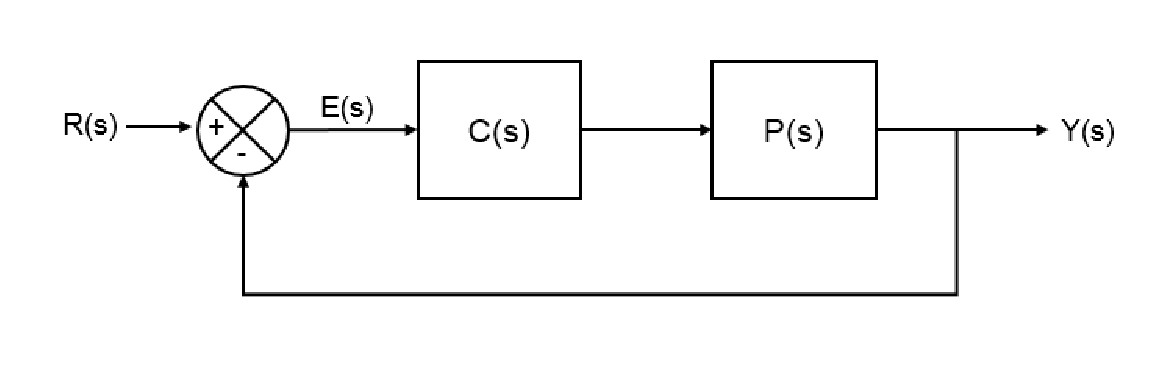
\includegraphics[width=0.5\textwidth]{figs/control_sistem}
\caption{Sistema de control con realimentaci�n unitaria}\label{sistem2ord}
\end{figure}

% ------------------------------------------------------------------------
Para efectos de ilustraci�n, se asumir� una planta gen�rica de segundo orden con un polo en el origen, a partir de:
% ------------------------------------------------------------------------
\begin{equation}
P(s)=\frac{1}{s(s+2)}=\frac{N(s)}{D(s)},\label{planta}
\end{equation}\
% ------------------------------------------------------------------------
definiendo a su vez el siguiente polinomio caracter�stico:
% ------------------------------------------------------------------------
\begin{eqnarray}
\nonumber \delta(s) & = & N(s)[k(s+\alpha)]+D(s)(s+\beta) \\
\nonumber           & = & k(s+\alpha)+s(s+\alpha)(s+\beta)\\
                    & = & s^{3}+(2+\beta)s^{2}+(2\beta+k)s+k\alpha,\label{eqcaract}
\end{eqnarray}\
% ------------------------------------------------------------------------
cuyas ra�ces establecen la estabilidad del sistema.\\

Como es bien sabido, el \emph{Criterio de estabilidad de Routh-Hurwitz} \citep{ogata2010} permite determinar las condiciones para la estabilidad absoluta de un sistema din�mico, mediante un m�todo tabulado que define la posici�n de las ra�ces en el plano, para un polinomio que representa el denominador de la funci�n de transferencia del sistema.\\

As� entonces, se aplica dicho criterio a partir de los siguientes pasos:
% ------------------------------------------------------------------------
\begin{itemize}
% ------------------------------------------------------------------------
% ------------------------------------------------------------------------
% ------------------------------------------------------------------------
\item[1.] \emph{Se escribe el polinomio caracter�stico en la forma $\delta(s) = 0$ y se verifican las condiciones para que todos sus coeficientes sean diferentes de cero y del mismo signo}. De esta manera, asumiendo una convenci�n positiva, los coeficientes de \eqref{eqcaract} ser�n mayores a cero si se cumplen las siguientes condiciones:
$$
\left(2+\beta\right)>0; \quad \left(2\beta+k\right)>0; \quad k\alpha>0,
$$
a partir de lo cual, asumiendo que $k > 0$ es un par�metro constante conocido, las condiciones para estabilidad recaen sobre los par�metros restantes $\left\{\alpha, \beta \right\}$, siendo:
\begin{equation}\label{primera}
\beta > -2; \quad \beta > -\frac{k}{2}; \quad \alpha > 0.
\end{equation}
% ------------------------------------------------------------------------
% ------------------------------------------------------------------------
% ------------------------------------------------------------------------
\item[2.] \emph{Se construye el arreglo de Routh y se analizan los elementos en la primera columna}. \emph{La condici�n necesaria y suficiente para que todas las ra�ces de \eqref{eqcaract} se encuentren en el semiplano izquierdo del plano ``$s$'', es que no existan cambios de signo en la primera columna del arreglo} \citep{ogata2010}. A partir de ello se tiene:
% ------------------------------------------------------------------------
\begin{center}
	\begin{tabular}{ l | c  c  }
		$s^{3}$ 	& 1                        & $\left(2\beta+k\right)$  \\
		$s^{2}$ 	& $\left(2+\beta\right)$   & $k\alpha$                \\
		$s^{1}$ 	& $M$                      & $ 0$                     \\
		$s^{0}$ 	& $k\alpha$                &                          \\
	\end{tabular}
\end{center}
% ------------------------------------------------------------------------
siendo
% ------------------------------------------------------------------------
\begin{eqnarray*}
M & = & \frac{\left(2\beta+k\right)\left(2+\beta\right)-k\alpha}{\left(2+\beta\right)},
\end{eqnarray*}
% ------------------------------------------------------------------------

de lo cual, $M>0$ implica
$$
(2\beta+k)(2+\beta)-k\alpha>0,
$$
puesto que $\left(2+\beta\right)>0$ y as� entonces:
$$
2\beta^{2}+\left(4+k\right)\beta+2k-k\alpha>0.
$$
Despejando $\alpha$ en la expresi�n anterior se obtiene:
% ------------------------------------------------------------------------
\begin{equation}
\alpha < \frac{2}{k}\left(\left(\beta+\frac{\left( k+4\right)}{4}\right)^{2} - \frac{\left(k-4\right)^2}{16}\right),\label{lim_alpha}
\end{equation}

tomando en cuenta que:
\begin{eqnarray*}
\frac{2\beta^{2}+\left(4+k\right)\beta+2k}{k} & = & \frac{2}{k}\left(\beta^{2}+\frac{\left(k+4\right) }{2}\beta+k\right)\\
& = & \frac{2}{k}\left(\beta^{2}+\frac{\left(k+4\right)}{2}\beta+\frac{\left(k+4\right)^2}{16}-\frac{\left(k+4\right)^2}{16}+k\right)\\
& = & \frac{2}{k}\left(\left(\beta+\frac{\left( k+4\right)}{4}\right)^{2} + \frac{16k -\left(k^2+8k+16\right)}{16}\right)\\
& = & \frac{2}{k}\left(\left(\beta+\frac{\left( k+4\right)}{4}\right)^{2} - \frac{\left(k^2-8k+16\right)}{16}\right)\\
& = & \frac{2}{k}\left(\left(\beta+\frac{\left( k+4\right)}{4}\right)^{2} - \frac{\left(k-4\right)^2}{16}\right). \label{stabsetlim}
\end{eqnarray*}
% ------------------------------------------------------------------------
% ------------------------------------------------------------------------
% ------------------------------------------------------------------------
\item[3.] \emph{A partir de las restricciones obtenidas sobre los t�rminos de la primera columna del arreglo de Routh, se determina el rango de valores que asegura para cada par�metro la estabilidad absoluta del sistema}. Por tanto, para $k > 4$ la condici�n que prevalece sobre el par�metro $\beta$ ser�:
    \begin{equation}
    \beta > -2.\label{stabset1}
    \end{equation}
    Asimismo se tiene:
    \begin{equation}
    0 < \alpha < \frac{2}{k}\left(\left(\beta+\frac{\left( k+4\right)}{4}\right)^{2} - \frac{\left(k-4\right)^2}{16}\right).\label{stabset2}
    \end{equation}
% ------------------------------------------------------------------------
\end{itemize}\

% ------------------------------------------------------------------------
\section{Conjunto estabilizante}\label{conjestabsect}
% ------------------------------------------------------------------------
\noindent Dada una estructura de controlador fija $C(s)$ para una planta $P(s)$, el conjunto estabilizante $\mathcal{S}$ se define como todos los posibles controladores $C(s)$ que brindan una soluci�n estable para el sistema realimentado mostrado en la Fig. \ref{sistem2ord}.\\

En este punto es importante resaltar que en la mayor�a de m�todos cl�sicos para el dise�o de controladores, el c�lculo de los par�metros del controlador se realiza sin incluir restricciones expl�citas de estabilidad. En general, un dise�o viene acompa�ado por pruebas de verificaci�n no s�lo para las condiciones de operaci�n del sistema controlado sino tambi�n para su estabilidad, constituyendo procedimientos iterativos muchas veces del tipo ensayo y error.\\

En otras palabras, los m�todos de dise�o se formulan para cumplir con condiciones de desempe�o sobre un sistema controlado estable, pero no toman en cuenta que a�n cuando matem�ticamente el controlador pueda satisfacer el problema, existe un conjunto restringido de par�metros de control que aseguran la estabilidad del sistema.\\

El conjunto establizante $\mathcal{S}$ es f�cil de definir. Por ejemplo, para la combinaci�n de planta y controlador dada por las ecuaciones \eqref{controlador}-\eqref{planta} en la Secci�n \ref{estabsect}, dicho conjunto puede escribirse como:
\begin{equation}
\mathcal{S} = \left\{\left(k, \alpha,\beta\right): \: \text{\eqref{stabset1} y \eqref{stabset2} se satisfagan simult�neamente} \right\}.\label{stabseteq}
\end{equation}

El conjunto estabilizante $\mathcal{S}$ es dificil de calcular. Para sistemas de bajo orden, el \emph{criterio de estabilidad de Routh-Hurwirtz} puede ser empleado seg�n ilustrado en la Secci�n \ref{estabsect}. Sin embargo, para un orden elevado la cantidad de expresiones no lineales que se requiere combinar para determinar los rangos de par�metros estables justifican la utilizaci�n de m�todos computacionales refinados. El \emph{m�todo de la signatura} propuesto por Keel y Bhattacharyya es una opci�n viable para estos casos \citep{keel2008}.

% ------------------------------------------------------------------------
\subsection{Incidencia de $\mathcal{S}$ en la estabilidad de un lazo de control}\label{lazoestable}
% ------------------------------------------------------------------------
\noindent Para verificar la importancia del conjunto estabilizante, considere el problema de dise�o de un compensador $C(s)$ de la forma \eqref{controlador} para el sistema $P(s)$ definido en \eqref{planta}, de manera tal que el sistema compensado y realimentado como en la Fig. \ref{sistem2ord} exhiba una respuesta escal�n con las siguientes caracter�sticas din�micas:
% ------------------------------------------------------------------------
\begin{equation}
M_p \approx 0\%; \quad t_s|_{2\%} \approx 0.5 \: [s].\label{spec}
\end{equation}\
% ------------------------------------------------------------------------

Inicialmente, se deben traducir las especificaciones de respuesta temporal dadas en \eqref{spec} al dominio de la frecuencia. A partir de ello, los polos deseados para el sistema compensado corresponden con:
% ------------------------------------------------------------------------
\begin{equation}
s = -8.231 \pm 0j \label{polo}.
\end{equation}\
% ------------------------------------------------------------------------

Ahora bien, evaluando este valor para ``$s$'' en $P(s)$, se verifica una deficiencia angular de:
% ------------------------------------------------------------------------
\begin{equation}
\angle C(s) = 180�,
\end{equation}
% ------------------------------------------------------------------------
que a su vez corresponde con la contribuci�n de fase que debe aportar el compensador en el polo deseado. A partir de ello, la localizaci�n para el polo y el cero del compensador se realiza empleando el siguiente an�lisis:
% ------------------------------------------------------------------------
\begin{itemize}
\item[-] Para obtener $180�$ de fase en el compensador, el cociente resultante debe ser un n�mero real negativo teniendo en cuenta el caracter real del polo deseado;
\item[-] Posteriormente se selecciona una distribuci�n en el eje real negativo para la localizaci�n del polo deseado y el polo y el cero del compensador, que conserve una simetr�a dada por un factor:
    $$
    \gamma = \frac{s}{5} \approx \frac{5}{3},
    $$
    en modo tal que:
    $$
    \alpha = \gamma s \approx 13.21, \quad \beta = \frac{s}{\gamma} \approx 4.84;
    $$
\item [-] Por �ltimo se determina la ganancia $k$ del compensador, como aquel valor que satisface
la condici�n de magnitud para el lugar geom�trico de las ra�ces:
% ------------------------------------------------------------------------
\begin{equation}
\left| \frac{k(s+13.21)}{s(s+2)(s+4.84)} \right|_{s=-8.231 \pm 0j}  =  1,
\end{equation}\
% ------------------------------------------------------------------------
a partir de lo cual $k \approx 34.93$.
% ------------------------------------------------------------------------
\end{itemize}\

% ------------------------------------------------------------------------
Una vez dise�ado el compensador, se procede a verificar el desempe�o del sistema controlado
empleando herramientas de simulaci�n. Es as� como la Fig. \ref{examp_inestable} muestra
la respuesta temporal ante un est�mulo de tipo escal�n unitario, calculada empleando el \emph{Control System Toolbox} de MATLAB\circledR~en el sistema compensado y realimentado,
siendo sin embargo de naturaleza inestable. A partir de lo anterior, surge la pregunta: �Por qu� un dise�o que se realiza empleando apropiadamente las herramientas matem�ticas, conduce a un sistema inestable?\\
% ------------------------------------------------------------------------
\begin{figure}[h]
\centering
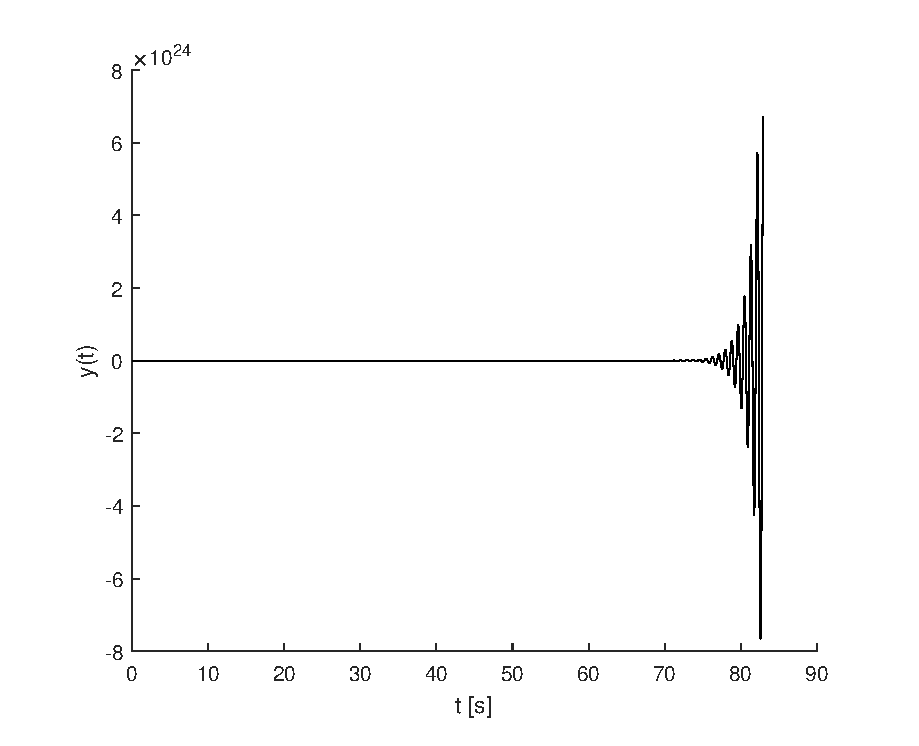
\includegraphics[width=0.5\textwidth]{figs/step_inestab}
\caption[Respuesta escal�n sistema compensado con inestabilidad]{Respuesta escal�n de sistema compensado manifestando inestabilidad}\label{examp_inestable}
\end{figure}

% ------------------------------------------------------------------------
La respuesta para este interrogante se explica f�cilmente a partir de \eqref{stabseteq}, justificando que los requerimientos dados en \eqref{spec} no son viables para la estructura del compensador seleccionada, seg�n se detalla a continuaci�n.

% ------------------------------------------------------------------------
\subsection{Escenarios din�micos viables en $\mathcal{S}$ para el sistema compensado}
% ------------------------------------------------------------------------
\noindent El conjunto estabilizante $\mathcal{S}$ definido en \eqref{stabseteq} depende de las inecuaciones \eqref{stabset1} y \eqref{stabset2}, establecidas a su vez para $k > 0$.\\

De los resultados presentados para el c�lculo del compensador se observa que $k = 34.93$ satisface la �ltima premisa. Por tanto, el controlador ser� estable si tanto $\alpha$ como $\beta$ satisfacen para este valor de $k$, las desigualdades que relacionan los elementos en la primera columna del arreglo de Routh.\\

As� entonces, reemplazando \eqref{primera}-\eqref{lim_alpha} para $k = 34.93$ en \eqref{stabset1} y \eqref{stabset2}, se obtiene:
% ------------------------------------------------------------------------
\begin{eqnarray*}
    \beta &=& 4.84\\
          &>& -2;\\
    \alpha &=& 13.21\\
           &>& 0\\
           & \nless& \frac{2}{34.93}\left(\left(4.84+\frac{\left( 34.93+4\right)}{4}\right)^{2} - \frac{\left(34.93-4\right)^2}{16}\right)\\
           & \nless& 8.73,
\end{eqnarray*}
% ------------------------------------------------------------------------
de donde la �ltima desigualdad muestra la raz�n por la cual el controlador calculado representa un sistema realimentado inestable.\\

De hecho, es posible graficar el plano de par�metros ($\alpha$, $\beta$) que representa los controladores con estructura \eqref{controlador} que para $k = 34.93$
garantizan la estabilidad del sistema controlado y realimentado. Dicha gr�fica se presenta en la Fig. \ref{conjestab1}, siendo el interior de la regi�n gris
el conjunto estabilizante $\mathcal{S}$, mientras el tri�ngulo indica el controlador calculado en la Secci�n \ref{lazoestable} evidenciando su condici�n de
realizaci�n inestable para el sistema.\\
% ------------------------------------------------------------------------

\begin{figure}[h]
\centering
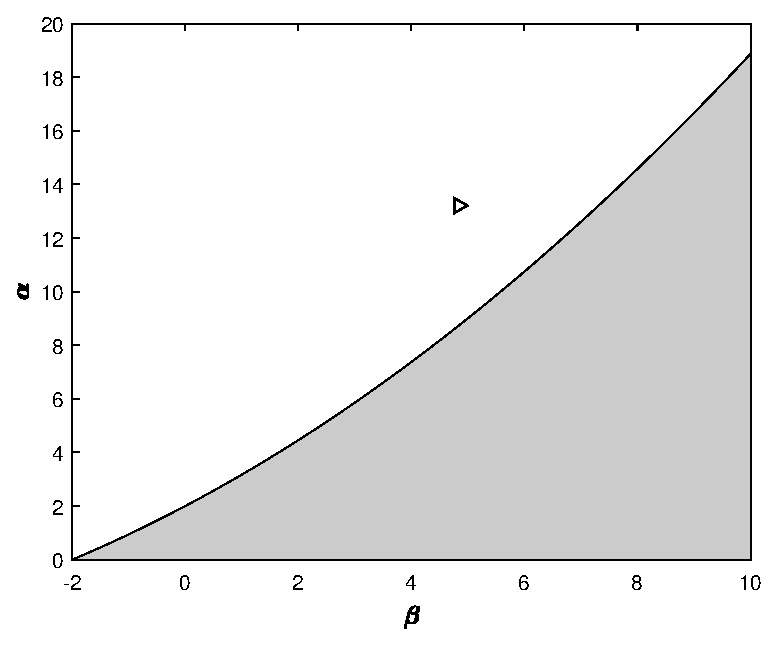
\includegraphics[width=0.5\textwidth]{figs/stab_set1}
\caption{Conjunto estabilizante en el plano ($\alpha$, $\beta$) para $k = 34.93$}\label{conjestab1}
\end{figure}
% ------------------------------------------------------------------------

M�s interesante a�n es transformar dicho conjunto estabilizante en t�rminos de par�metros del controlador hacia un espacio de especificaciones de desempe�o. Por ejemplo, observe en la Fig. \ref{Mp-ts} el plano ($M_p$, $t_s$) equivalente para el conjunto estabilizante mostrado en la Fig. \ref{conjestab1}.\\

De este diagrama se observa la manera en la cual los par�metros de desempe�o requeridos para el dise�o presentado en la Secci�n \ref{lazoestable}, no forman parte de los escenarios din�micos viables en el conjunto estabilizante para el sistema compensado. Visualmente se observa una discontinuidad del conjunto $\mathcal{S}$ al ser mapeado desde el plano ($\alpha$, $\beta$) hacia el plano ($M_p$, $t_s$). Un an�lisis detallado del efecto anterior involucra \emph{topolog�a matem�tica}, superando los alcances del presente trabajo de grado.\\

% ------------------------------------------------------------------------

\begin{figure}[h]
\centering
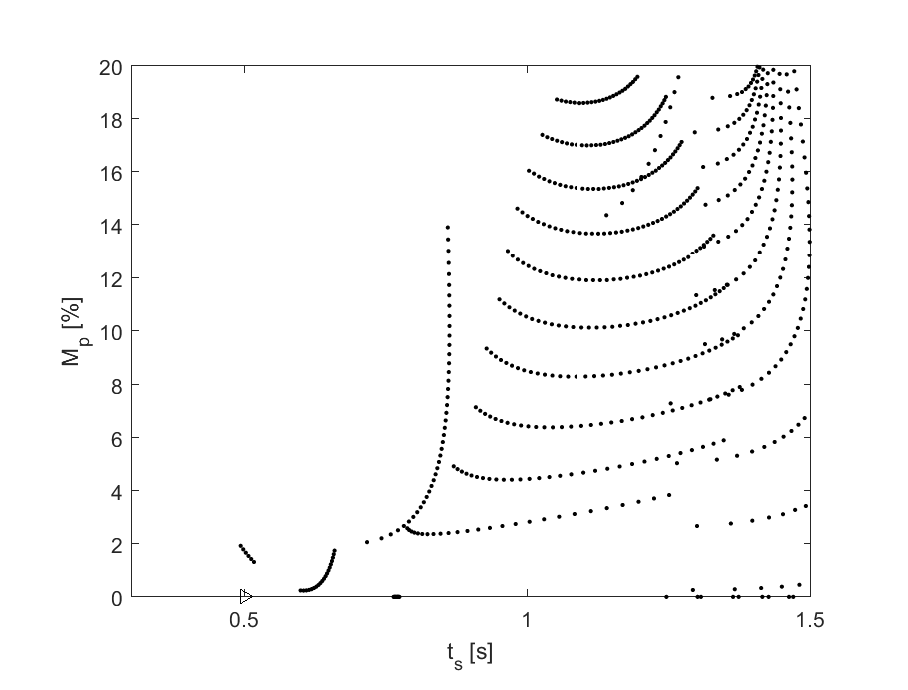
\includegraphics[width=0.7\textwidth]{figs/Mp_ts}
\caption{Conjunto estabilizante en el plano ($M_p$, $t_s$) para $k = 34.93$}\label{Mp-ts}
\end{figure}
% ------------------------------------------------------------------------

Por tanto, dada la dificultad matem�tica que implica un mapeo anal�tico entre el conjunto estabilizante $\mathcal{S}$ y los par�metros de una respuesta escal�n, el plano presentado en la Fig. \ref{Mp-ts} fue generado empleando simulaci�n de fuerza bruta (es decir, punto a punto) a partir de las funciones del \emph{Control Systems Toolbox} de MATLAB\circledR.\\

De esta manera es posible realizar una selecci�n visual para los par�metros del controlador (\emph{m�todo gr�fico de dise�o}) a partir de una elecci�n de las especificaciones de desempe�o requeridas en la respuesta escal�n, al interior del conjunto admisible dado en la Fig. \ref{Mp-ts}\\

La Fig. \ref{respuestas} ilustra la selecci�n para varios escenarios din�micos al interior de la regi�n de estabilidad, con su correspondiente mapeo al plano de par�metros del controlador.\\
% ------------------------------------------------------------------------
\begin{figure}
\centering
	\subfigure[$M_p = 53.38; \: t_s = 3.60$]{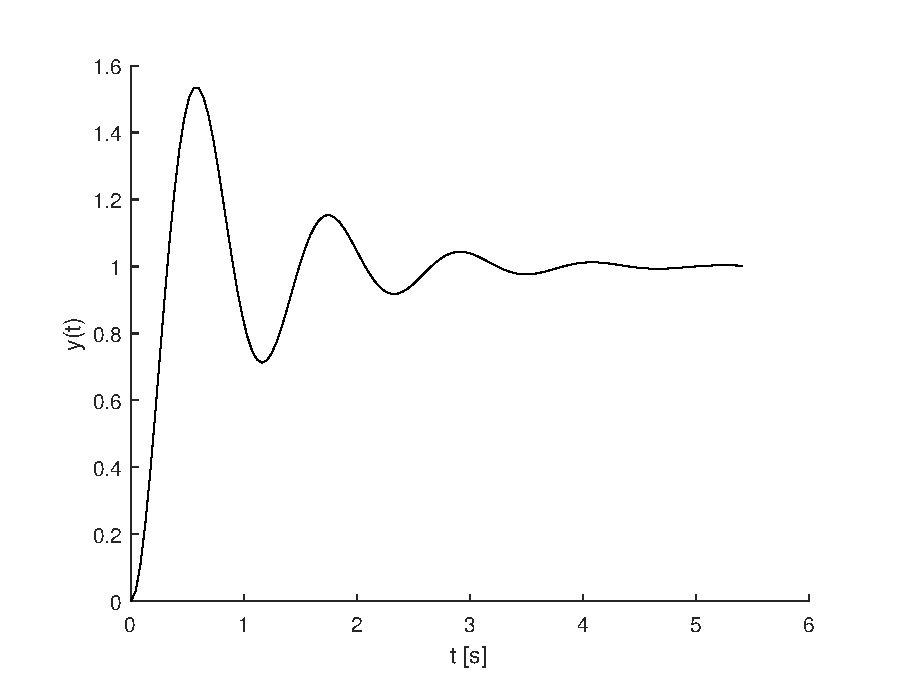
\includegraphics[width=0.45\textwidth]{Figs/step_E1}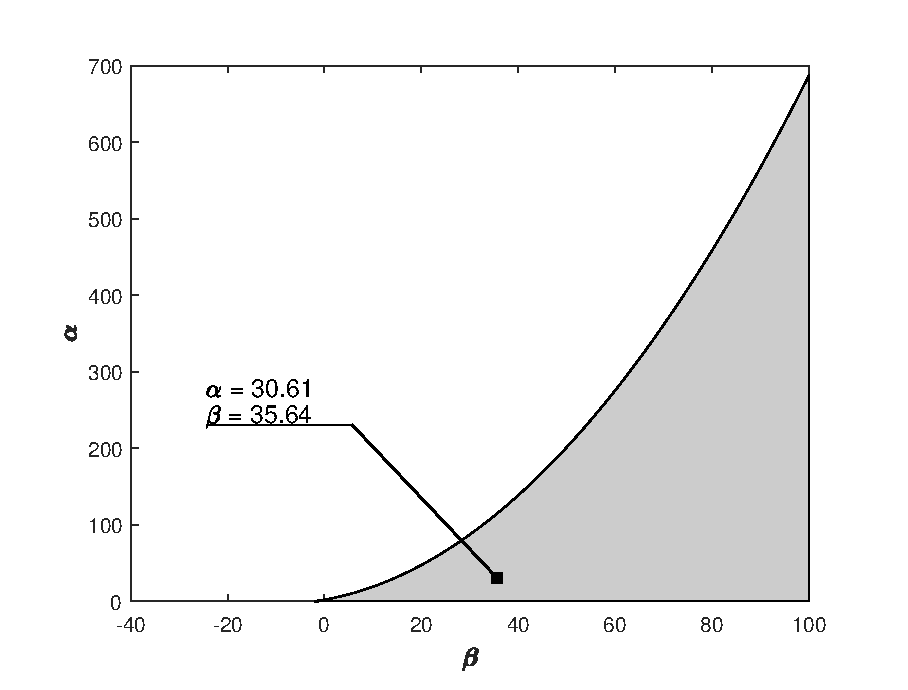
\includegraphics[width=0.45\textwidth]{Figs/stab_set_E1}}
	\subfigure[$M_p = 70.76; \: t_s = 4.59$]{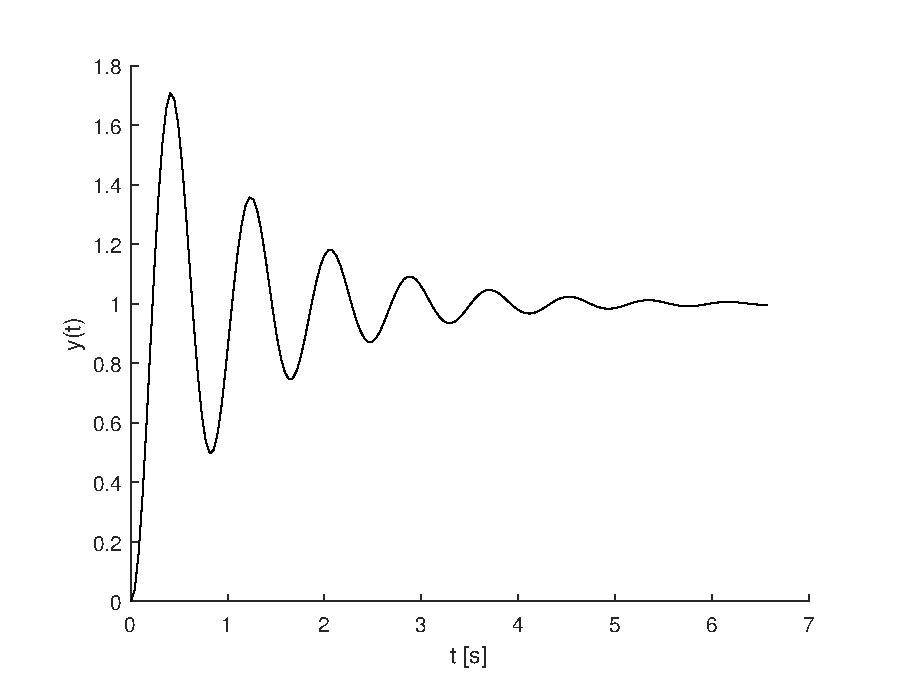
\includegraphics[width=0.45\textwidth]{Figs/step_E2}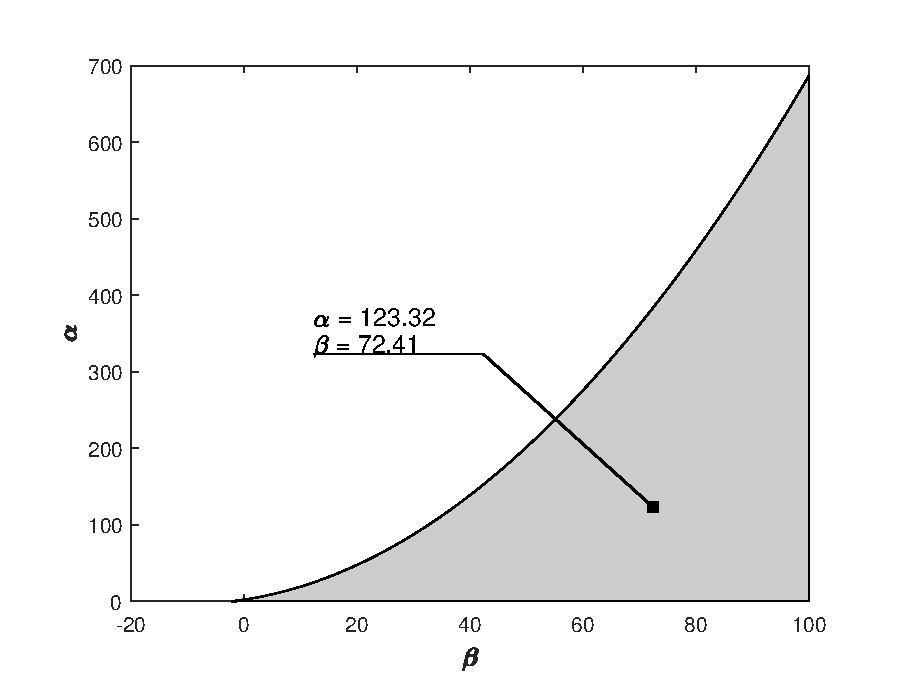
\includegraphics[width=0.45\textwidth]{Figs/stab_set_E2}}
	\subfigure[$M_p = 84.76; \: t_s = 6.85$]{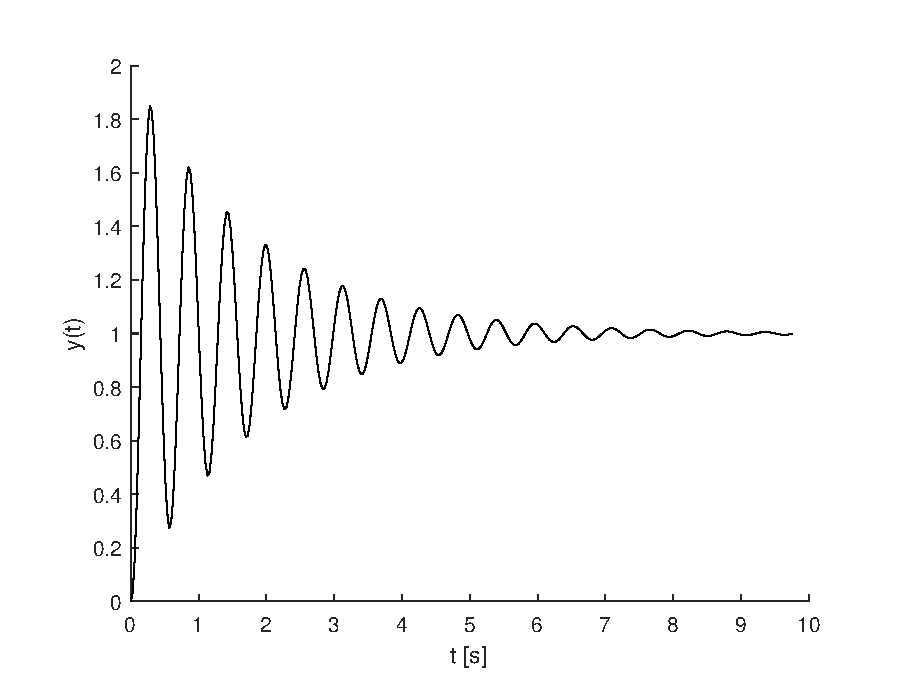
\includegraphics[width=0.45\textwidth]{Figs/step_E3}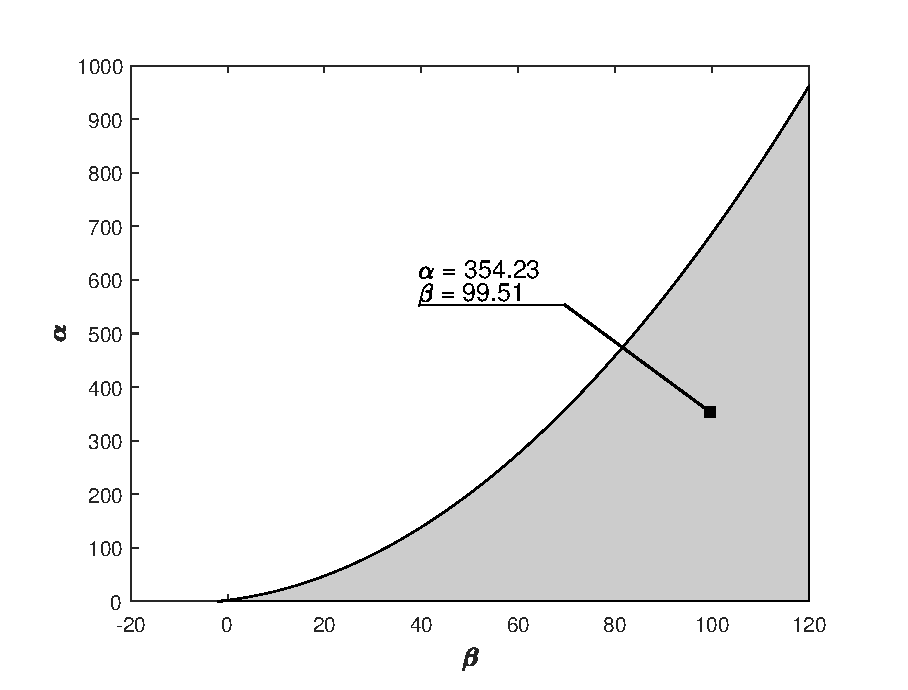
\includegraphics[width=0.45\textwidth]{Figs/stab_set_E3}}
\caption[Respuesta din�mica y controlador en $\mathcal{S}$ del plano ($M_p$, $t_s$)]{Respuesta din�mica y controlador correspondiente para diferentes especificaciones al interior de $\mathcal{S}$ en el plano ($M_p$, $t_s$)}\label{respuestas}
\end{figure}

% ------------------------------------------------------------------------
A partir de lo anterior, pueden emplearse herramientas computacionales para realizar, de manera gr�fica, el c�lculo de un compensador de estructura predeterminada para una planta conocida y con base en el conjunto de especificaciones de desempe�o admisible proporcionadas por el conjunto estabilizante, seg�n se detalla en la siguiente secci�n.

% ------------------------------------------------------------------------
\section{Dise�o gr�fico de controladores a partir del c�lculo de $\mathcal{S}$}\label{interfazsect}
% ------------------------------------------------------------------------
% ------------------------------------------------------------------------
\noindent Tomando en cuenta la alta capacidad de c�lculo y portabilidad de las herramientas computacionales actuales, resulta simple aceptar que las dificultades anal�ticas en la determinaci�n de par�metros de control puedan ser reducidas ostensiblemente a partir de paquetes como MATLAB, que integra funciones optimizadas para aproximar con muy alta precisi�n los valores de variables importantes en un sistema de control realimentado, ante simulaci�n para diversos escenarios de operaci�n.\\

Tomando en cuenta lo anterior, se construy� una interfaz para realizar el dise�o de controladores simples (i.e. compensadores en adelanto o en atraso), a partir de un enfoque gr�fico basado en el c�lculo del conjunto estabilizante para sistemas \emph{SISO LTI}. El dise�o de la interfaz se presenta a continuaci�n empleando como base la descripci�n propuesta por Roa y Ayala en \citep{roa_ayala2016} para este tipo de desarrollos.

% ------------------------------------------------------------------------
\subsection{Descripci�n general de requerimientos}
% ------------------------------------------------------------------------
\noindent Se requiere construir una interfaz de software que permita dise�ar un controlador de estructura simple pre-establecida, a partir de informaci�n del conjunto admisible de par�metros de respuesta din�mica, calculados con base en el conjunto estabilizante $\mathcal{S}$ para un sistema realimentado de manera negativa y unitaria. La interfaz deber� permitir modificar la ganancia $k$ de baja frecuencia del controlador, as� como los rangos de variaci�n del par�metro $\beta$ y la resoluci�n de puntos para el conjunto estabilizante calculado, permitiendo visualizar dicho conjunto en el plano $\left(\alpha,\beta\right)$, su mapeo correspondiente hacia el plano de par�metros de respuesta $\left(M_p, t_s \right)$ y la respuesta escal�n del sistema realimentado para un punto arbitrario dentro de $\mathcal{S}$.

% ------------------------------------------------------------------------
\subsubsection{Nivel superior de detalle}
% ------------------------------------------------------------------------
\noindent Posterior a la descripci�n (en palabras) de los requerimientos del sistema (interfaz), se procede a  crear un diagrama general de entradas y salidas a manera de nivel superior de detalle. Dicha representaci�n se muestra en la Fig. \ref{Nsuperior}.
% ------------------------------------------------------------------------
\begin{figure}[h]
\centering
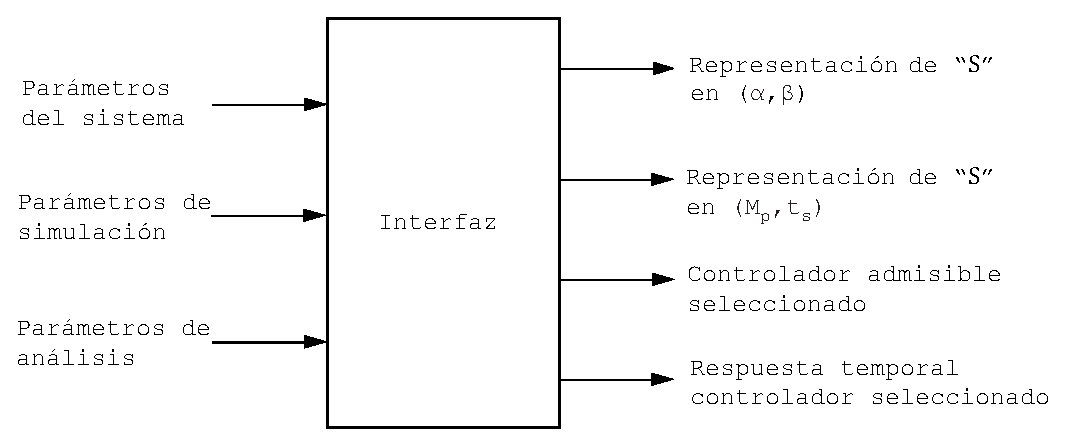
\includegraphics[width=0.7\textwidth]{figs/Nivel_superior}
\caption[Nivel superior de detalle para desarrollo de interfaz]{Representaci�n de nivel superior de detalle para desarrollo de interfaz}\label{Nsuperior}
\end{figure}
% ------------------------------------------------------------------------

\subsubsection{Partici�n de primer nivel}
% ------------------------------------------------------------------------
\noindent Una primera partici�n se logra con la incorporaci�n del bloque que realiza el c�lculo del conjunto estabilizante $\mathcal{S}$, mediante evaluaci�n de las expresiones \eqref{stabset1}, \eqref{stabset2} y \eqref{stabseteq}.\\
% ------------------------------------------------------------------------
\begin{figure}[h]
\centering
\includegraphics[width=1.0\textwidth]{figs/Primer_nivel}
\caption[Primer nivel de detalle para desarrollo de interfaz]{Representaci�n de primer nivel de partici�n para desarrollo de interfaz}\label{Nprimer}
\end{figure}\
% ------------------------------------------------------------------------

Asimismo, los resultados en esta etapa son la informaci�n de entrada a un nuevo bloque encargado de construir la representaci�n gr�fica del conjunto estabilizante en el espacio de par�metros $\left(M_p, t_s \right)$. Lo anterior se realiza en una secuencia de dos pasos: \emph{1)} se calculan las respuestas escal�n $y(t)$ para el sistema realimentado con cada uno de los par�metros de controlador dados por $\mathcal{S}$ y \emph{2)} se determina el valor correspondiente en el plano $\left(M_p, t_s \right)$ para cada caso.\\

Con esta informaci�n, el usuario puede proceder a seleccionar un punto admisible $\left(M_p^*, t_s^* \right)$, que posteriormente es representado en su versi�n equivalente de par�metros del controlador deseado $\left(\alpha^*,\beta^* \right)$. Finalmente, se calcula para este punto la respuesta escal�n $y^*(t)$ para el sistema realimentado.\\

De esta manera, el primer nivel de partici�n se configura con la uni�n de los anteriores subprocesos, tal y como se ilustra en la Fig. \ref{Nprimer}.

% ------------------------------------------------------------------------
\subsubsection{Particiones de segundo nivel}
% ------------------------------------------------------------------------
\noindent A su vez, cada uno de los subprocesos descritos en el �tem anterior, se descompone en etapas constitutivas fundamentales seg�n se describe a continuaci�n:
% ------------------------------------------------------------------------
\begin{itemize}
% ------------------------------------------------------------------------
\item[-] \emph{C�lculo de $\mathcal{S}$}: para determinar el conjunto estabilizante se debe establecer para un $k$ dado y un intervalo de variaci�n conocido para $\beta$, el rango de $M$ valores para la variable $\alpha$ que satisface las restricciones impuestas por las ecuaciones \eqref{stabset1}, \eqref{stabset2} y \eqref{stabseteq}. El esquema para estas subrutinas se muestra en la Fig. \ref{Nsegundo1};
\item[-] \emph{C�lculo respuesta escal�n a partir de $\left(\alpha,\beta\right)$}: una vez calculado $\mathcal{S}$, es posible evaluar cada punto $\left(\alpha,\beta\right)$ en la estructura de control realimentado mostrada en la Fig. \ref{sistem2ord}. De esta manera puede calcularse, a trav�s de comandos del \emph{Control System Toolbox} de MATLAB, la respuesta escal�n para el sistema. El esquema para estas subrutinas se muestra en la Fig. \ref{Nsegundo2};
\item[-] \emph{Elecci�n de punto admisible en $\left(M_p, t_s \right)$}: a trav�s de selecci�n gr�fica el usuario seleccionar� un punto de inter�s $\left(\bar{M_p}, \bar{t_s} \right)$. Posteriormente, se deber� verificar si dicho punto pertenece al conjunto de par�metros admisibles $\left(M_p, t_s \right)$. En caso afirmativo, el punto se denominar� $\left(M_p^*, t_s^* \right)$. El esquema para estas subrutinas se muestra en la Fig. \ref{Nsegundo3};
\item[-] \emph{Conversi�n punto $\left(M_p^*, t_s^* \right)$ a punto $\left(\alpha,\beta\right)$ dentro de $\mathcal{S}$}: tomando en cuenta que los planos $\left(M_p, t_s \right)$ y $\left(\alpha,\beta\right)$ poseen las mismas dimensiones y son una relaci�n uno a uno, la posici�n del punto $\left(M_p^*, t_s^* \right)$ equivale al conjunto de par�metros $\left(\alpha^*,\beta^* \right)$ del controlador que lo produce. El esquema para estas subrutinas se muestra en la Fig. \ref{Nsegundo4}.
% ------------------------------------------------------------------------
\end{itemize}
% ------------------------------------------------------------------------
\begin{figure}[h]
\centering
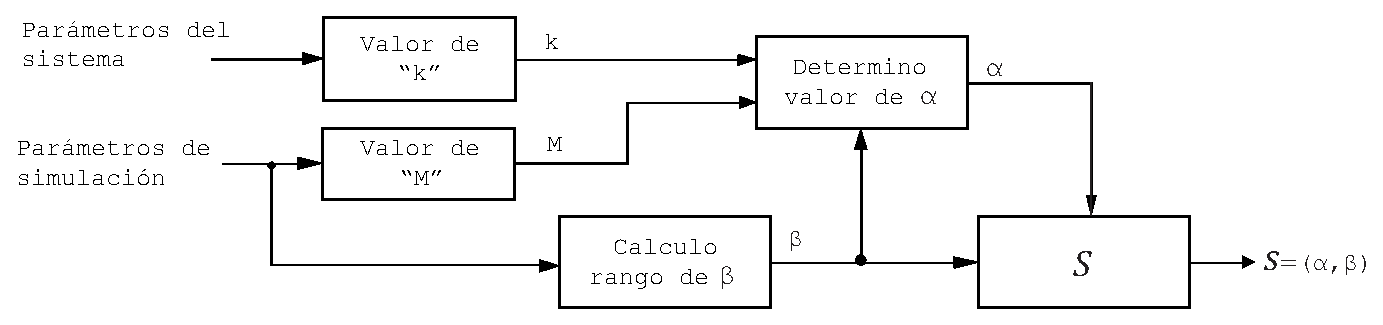
\includegraphics[width=0.8\textwidth]{figs/Segundo_Nivel_Sub_1}
\caption[Subproceso de \emph{C�lculo de $\mathcal{S}$}]{Representaci�n de segundo nivel de partici�n para subproceso de \emph{C�lculo de $\mathcal{S}$}}\label{Nsegundo1}
\end{figure}
% ------------------------------------------------------------------------
\begin{figure}[h]
\centering
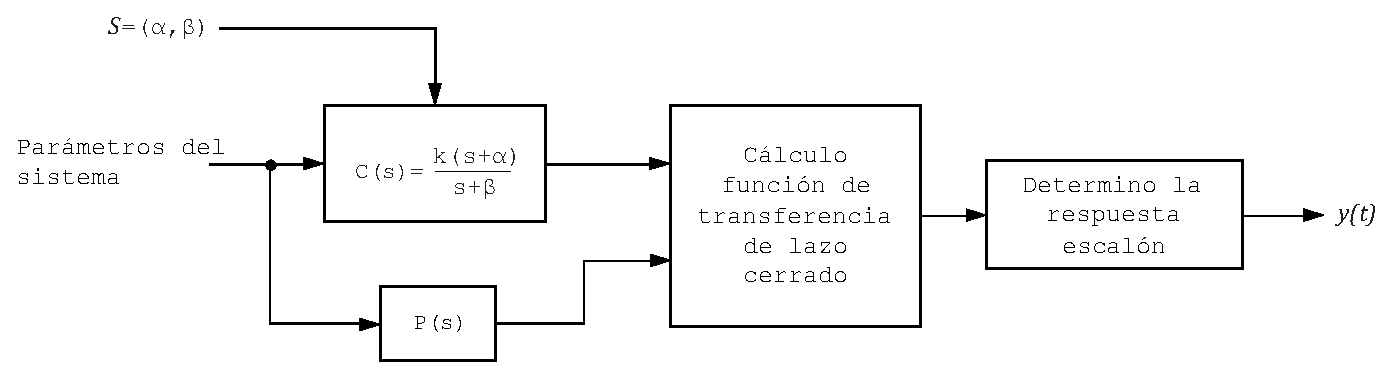
\includegraphics[width=0.8\textwidth]{figs/Segundo_Nivel_Sub_2}
\caption[Subproceso de \emph{C�lculo respuesta escal�n a partir de $\left(\alpha,\beta\right)$}]{Representaci�n de segundo nivel de partici�n para subproceso de \emph{C�lculo respuesta escal�n a partir de $\left(\alpha,\beta\right)$}}\label{Nsegundo2}
\end{figure}
% ------------------------------------------------------------------------
\begin{figure}[h]
\centering
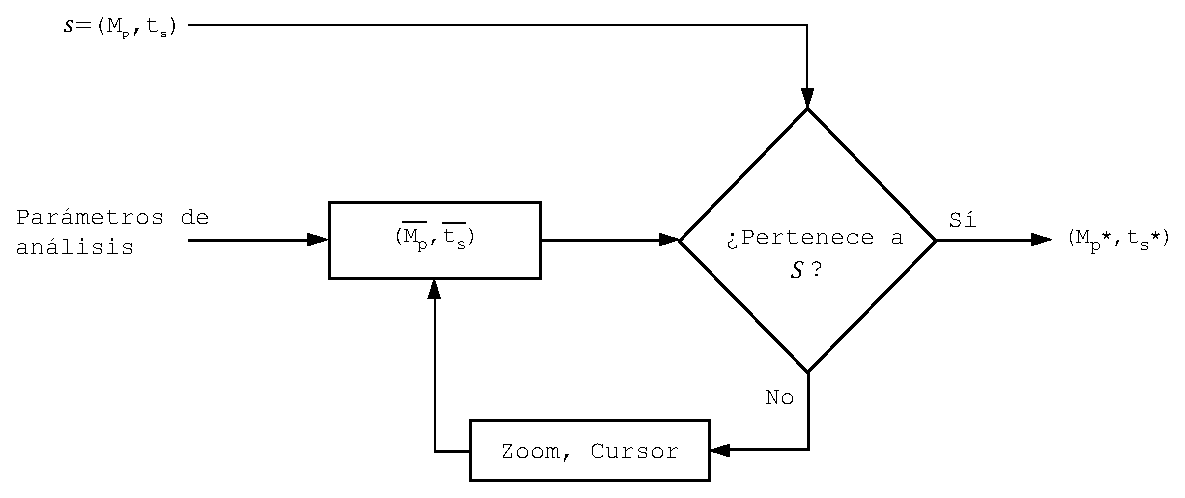
\includegraphics[width=0.8\textwidth]{figs/Segundo_Nivel_Sub_3}
\caption[Subproceso de \emph{Elecci�n de punto admisible en $\left(M_p, t_s \right)$}]{Representaci�n de segundo nivel de partici�n para subproceso de \emph{Elecci�n de punto admisible en $\left(M_p, t_s \right)$}}\label{Nsegundo3}
\end{figure}
% ------------------------------------------------------------------------
\begin{figure}[h]
\centering
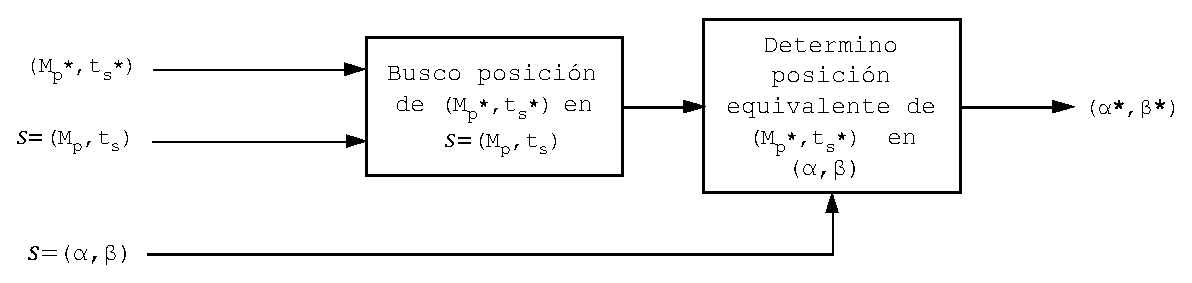
\includegraphics[width=0.8\textwidth]{figs/Segundo_Nivel_Sub_4}
\caption[Subproceso de \emph{Conversi�n $\left(M_p^*, t_s^* \right)$ a $\left(\alpha,\beta\right)$}]{Representaci�n de segundo nivel de partici�n para subproceso de \emph{Conversi�n punto $\left(M_p^*, t_s^* \right)$ a punto $\left(\alpha,\beta\right)$ dentro de $\mathcal{S}$}}\label{Nsegundo4}
\end{figure}
% ------------------------------------------------------------------------

El esquema definitivo para las etapas que constituyen la interfaz, implica la combinaci�n de los esquemas presentados en las Figs. \ref{Nprimer} y \ref{Nsegundo1}-\ref{Nsegundo4}.

% ------------------------------------------------------------------------
\subsection{Selecci�n de herramienta para implementaci�n}
% ------------------------------------------------------------------------
\noindent A partir del diagrama obtenido en la Fig. \ref{Nprimer}, es claro que el coraz�n de la interfaz a ser dise�ada es la rutina que calcula los par�metros de respuesta escal�n en el sistema compensado para cada punto de prueba. Como ya mencionado, estas tareas facilitan su ejecuci�n empleando los comando del \emph{Control System Toolbox} de MATLAB. Por tanto, se considera a dicha herramienta como la primera opci�n para desarrollar la interfaz de software requerida.\\

Mas a�n, MATLAB posee adem�s de la consola de comandos y el entorno de programaci�n gr�fico SIMULINK, un entorno para el desarrollo de interfaces de usuario denominado GUIDE (Graphical User Interface Development Environment).\\

Tomando en cuenta lo anterior, se selecciona MATLAB \emph{vR2017a} para construir la interfaz de usuario que satisface los requerimientos de dise�o ilustrados en los diagramas de nivel de partici�n previamente presentados.

% ------------------------------------------------------------------------
\subsection{Descripci�n de interfaz dise�ada}
% ------------------------------------------------------------------------
\begin{figure}
\centering
\includegraphics[width=1.0\textwidth]{figs/interfaz}
\caption{Presentaci�n final para interfaz desarrollada}\label{interfaz}
\end{figure}
% ------------------------------------------------------------------------

\noindent Procediendo con el dise�o, se realiza codificaci�n en MATLAB para la combinaci�n de los diagramas de bloques de las Figs. \ref{Nprimer}-\ref{Nsegundo4}, asumiendo las siguientes \emph{variables de entrada}:
% ------------------------------------------------------------------------
\begin{itemize}
    \item Par�metros de simulaci�n: [$\beta_{min}$, $\beta_{max}$, $M$, $N$];
    \item Par�metros del sistema: [$k$, $P(s)$, estructura para $C(s)$];
    \item Par�metros de an�lisis: [$\bar{M_p}$, $\bar{t_s}$],
\end{itemize}
% ------------------------------------------------------------------------
y \emph{de salida}:
% ------------------------------------------------------------------------
\begin{itemize}
	\item Representaci�n de $\mathcal{S}$ en $\left(\alpha,\beta\right)$: [$\mathcal{S} = \left(\alpha,\beta\right)$];
    \item Representaci�n de $\mathcal{S}$ en $\left(M_p,t_s\right)$: [$\mathcal{S} = \left(M_p,t_s\right)$];
    \item Controlador admisible seleccionado: [$\left(\alpha^*,\beta^* \right)$];
    \item Respuesta temporal controlador seleccionado: [$y^*(t)$].
\end{itemize}\
% ------------------------------------------------------------------------

Todo lo anterior fue adecuado como se presenta en la Fig. \ref{interfaz}, ilustrando la presentaci�n final de la interfaz desarrollada.
% ------------------------------------------------------------------------
% ------------------------------------------------------------------------    % Conjunto estabilizante para sistemas LTI
% ------------------------------------------------------------------------
% ------------------------------------------------------------------------
% ------------------------------------------------------------------------
%                                Cap�tulo 3
% ------------------------------------------------------------------------
% ------------------------------------------------------------------------
% ------------------------------------------------------------------------

\chapter{Modelado matem�tico del dron}
% ------------------------------------------------------------------------
\noindent En el presente Cap�tulo se formula el conjunto de ecuaciones
diferenciales que describen el comportamiento din�mico del \emph{dron}; es decir,
su modelo matem�tico. Partiendo de principios f�sicos y trigonom�tricos
fundamentales, se estudia el movimiento de la part�cula en el espacio a
partir de simulaci�n num�rica de modelos efectuada en MATLAB. Esta
informaci�n del comportamiento temporal del sistema, ser� base para el dise�o
de estrategias de control abordadas en Capitulos posteriores.
% ------------------------------------------------------------------------

\section{Veh�culos a�reos no tripulados}
% ------------------------------------------------------------------------
\noindent La siguiente descripci�n general de veh�culos a�reos no tripulados (UAV del ingl�s unmanned aerial vehicles) del tipo cuadrotor, es una adaptaci�n de los contenidos reportados a manera de revisi�n en \citep{reviewieee}.\\

Los cuadric�pteros o cuadrotores (ver Fig. \ref{drone}), son un tipo �nico de UAV que posee la habilidad de despegue y aterrizaje vertical. Este tipo de veh�culo se considera un sistema subactuado, debido a que posee menos entradas que salidas, lo cual lo hace un reto desde el punto de vista del control de su din�mica. Hist�ricamente los UAV fueron concebidos para la industria militar. Sin embargo, actualmente el abaratamiento de costos y desarrollo de materiales han permitido masificar su uso en aplicaciones civiles con popularidad en aumento.
% ------------------------------------------------------------------------
\begin{figure}[h]
\centering
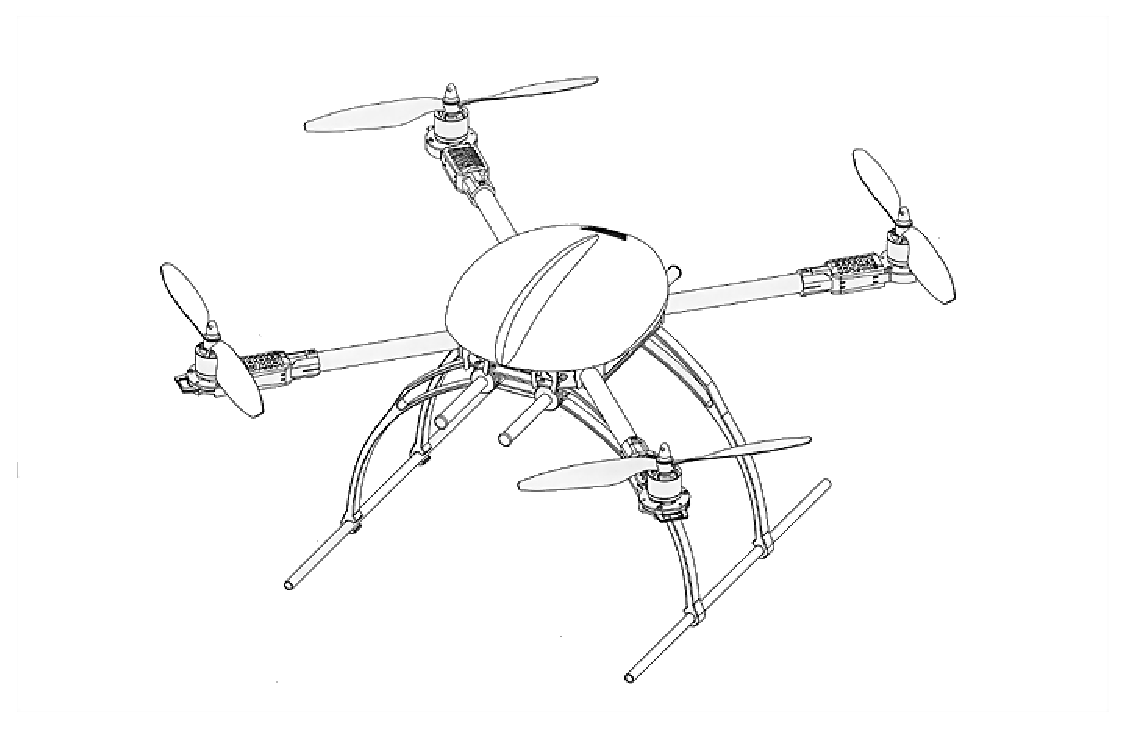
\includegraphics[width=0.5\textwidth]{figs/drone}
\caption{Veh�culo a�reo no tripulado tipo \emph{dron} cuadrotor}\label{drone}
\end{figure}\

% ------------------------------------------------------------------------
\subsection{Mecanismo de vuelo}
% ------------------------------------------------------------------------
\noindent La mayor diferencia entre un cuadrotor y un helic�ptero tradicional est� en su modo de propulsi�n de rotor fijo, en el cual la direcci�n de navegaci�n en cualquiera de sus ejes puede variar con s�lo modificar la propulsi�n a partir de una cierta combinaci�n de velocidad en sus motores. La distribuci�n de los cuatro motores puede realizarse en forma de $x$ o de $+$, teniendo cada una sus respectivas ventajas.\

% ------------------------------------------------------------------------
\subsection{Control del sistema}
% ------------------------------------------------------------------------
\noindent Con el aumento de posibilidades de uso de veh�culos UAV tipo cuadrotor, se han verificado progresos en los algoritmos orientados a una mayor maniobrabilidad y efectividad en aplicaciones cada vez m�s complejas. En la literatura t�cnica se reportan t�cnicas de control aplicadas en cuadrotores que van desde control PID elemental hasta controladores basados en redes neuronales. Asimismo, ha sido interesante la comparaci�n realizada entre el comportamiento de especies de la naturaleza y este tipo de veh�culo, en la b�squeda por sincronizar operaci�n colaborativa explotando su versatilidad y velocidad de respuesta.\

% ------------------------------------------------------------------------
\subsection{Sens�rica}
% ------------------------------------------------------------------------
\noindent A nivel de tecnolog�a, desarrollos en materiales y miniaturizaci�n electr�nica han permitido dotar cuadrotores con dispositivos como sistemas microelectromec�nicos (MEMs), unidades de medida inercial (IMUs) y sistemas de posicionamiento geoestacionario (GPS). Algunas aplicaciones tambi�n adicionan sistemas de visi�n y localizaci�n basada en radiofrecuencia. A pesar de ello, la precisi�n en las trayectorias del dispositivo y la estabilidad ante condiciones adversas de operaci�n (principalmente de tipo clim�tico) a�n imponen restricciones en la operaci�n del sistema.\

% ------------------------------------------------------------------------
\subsection{Aplicaciones}
% ------------------------------------------------------------------------
\noindent Una aeronave tripulada est� limitada por las habilidades y la fatiga del piloto. Desde ese punto de vista, la automatizaci�n de un cuadrotor permite emplearlos en aplicaciones donde sea latente el riesgo o se perjudique la integridad humana. Piense por ejemplo en una expedici�n al cr�ter de un volc�n o el sobrevuelo de un �rea contaminada por radioactividad. El potencial para este tipo de aplicaciones depende del entendimiento de la operaci�n del sistema a trav�s de la formulaci�n de modelos matem�ticos adecuados, tal y como se describe a continuaci�n.\\
% ------------------------------------------------------------------------

\section{Coordenadas en el espacio de movimiento}\label{modelodron}
% ------------------------------------------------------------------------
\noindent Formular las ecuaciones que describen el modelo din�mico del \emph{dron}
implica definir sus coordenadas en el espacio de movimiento. Cuando un objeto
gira alrededor de un eje, el an�lisis del movimiento puede simplificarse si se
considera un cuerpo r�gido; es decir, formado por varias part�culas puntuales que
guardan distancias constantes entre si \citep{sears2005fisica}.\\

Por tanto, asumiendo que el \emph{dron} de la Fig. \ref{drone} es un cuerpo r�gido,
su din�mica se describe en el espacio de movimiento a trav�s de tres cantidades
principales ilustradas en la Fig. \ref{cuerpolibre}, correspondientes con los
�ngulos de: 1) balanceo $\phi$ (roll), 2) cabeceo $\theta$ (pitch) y 3) gui�ada
$\psi$ (yaw). Estos �ngulos se miden en un sistema de referencia fijo con respecto
a la tierra (o inercial), denotado como $O$ y definido con base en los ejes
coordenados $\left( \vec{x}_O, \vec{y}_O, \vec{z}_O \right)$. A su vez, se
considera un sistema  variante en el tiempo alineado con el cuerpo del \emph{dron}
y denotado como $B$ en la Fig. \ref{cuerpolibre}, con centro de masa en el origen
de sus ejes coordenados $\left(\vec{x}_B, \vec{y}_B, \vec{z}_B \right)$.\\
% ------------------------------------------------------------------------
\begin{figure}[h]
\centering
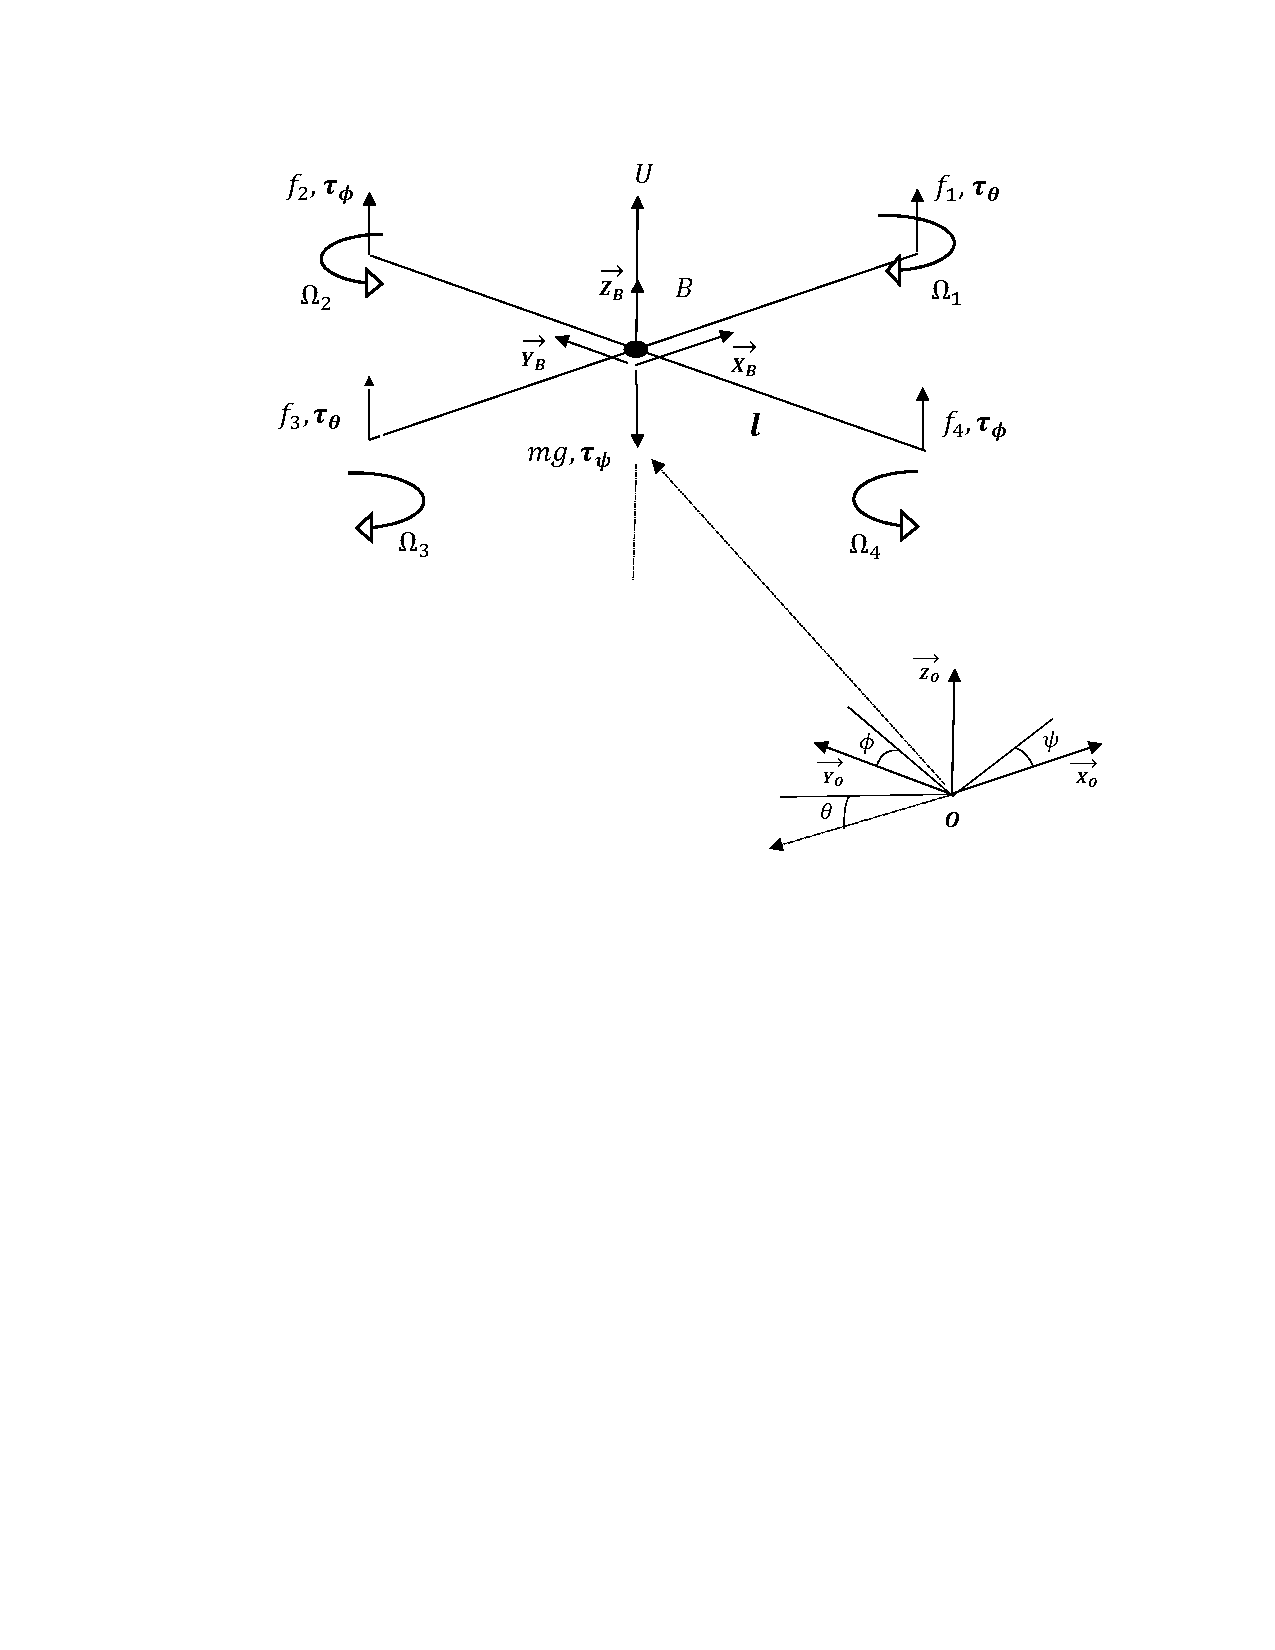
\includegraphics[width=0.7\textwidth]{figs/cuerpolibre}
\caption[Diagrama de cuerpo libre del \emph{dron} cuadrotor]{Diagrama de cuerpo 
libre del \emph{dron} cuadrotor. Adaptado de \citep{raffo2007modelado}}\label{cuerpolibre}
\end{figure}
% ------------------------------------------------------------------------

Para transformar las coordenadas de un punto entre el marco de referencia
del cuerpo y el marco de referencia inercial, se utiliza la expresi�n:
% ------------------------------------------------------------------------
\begin{equation}\label{ecuacion}
\begin{bmatrix}
  x_O \\
  y_O \\
  z_O
\end{bmatrix}
  =\mathbf{R}
  \begin{bmatrix}
    x_B \\
    y_B \\
    z_B
  \end{bmatrix},
 \end{equation}
% ------------------------------------------------------------------------
donde \citep{spong2008robot}:
% ------------------------------------------------------------------------
$$
\mathbf{R} = \begin{bmatrix}
\cos\psi\cos\theta &\cos\psi\sin\theta\sin\phi-\sin\psi\cos\phi   & \cos\psi\sin\theta\cos\phi+\sin\psi\sin\phi \\
\sin\psi\cos\theta &\sin\psi\sin\theta\sin\phi +\cos\psi\cos\phi   &\sin\psi\sin\theta\cos\phi-\cos\psi\sin\phi \\
 -\sin\theta&\cos\theta\sin\phi  &\cos\theta\cos\phi
\end{bmatrix}.
$$\
% ------------------------------------------------------------------------

Asimismo, es posible definir una relaci�n entre el vector de velocidades
angulares en el marco de referencia del cuerpo:
% ------------------------------------------------------------------------
$$
\mathbf{\nu} = \begin{bmatrix}
                 p \\
                 q \\
                 r
               \end{bmatrix},
$$
% ------------------------------------------------------------------------
con respecto a la variaci�n temporal de los �ngulos en el marco de
referencia inercial:
% ------------------------------------------------------------------------
$$
\mathbf{\eta} = \begin{bmatrix}
                  \dot{\phi} \\
                   \dot{\theta} \\
                    \dot{\psi}
                \end{bmatrix},
$$
% ------------------------------------------------------------------------
a partir de la siguiente expresi�n:
% ------------------------------------------------------------------------
\begin{equation}\label{velrela}
\mathbf{\nu} = \mathbf{W} \mathbf{\eta},
\end{equation}
% ------------------------------------------------------------------------
siendo \citep{spong2008robot}:
% ------------------------------------------------------------------------
$$
\mathbf{W} = \begin{bmatrix}
1 &0  &-\sin\theta \\
 0&\cos\phi  &\sin\phi\cos\theta \\
 0&-\sin\phi  &\cos\phi\cos\theta
\end{bmatrix}.
$$\
% ------------------------------------------------------------------------

Las matrices de transformaci�n de coordenadas $\mathbf{R}$ y $\mathbf{W}$
son ortogonales; es decir, son matrices cuadradas cuya matriz inversa
coincide con su matriz transpuesta \citep{stanley1993algebra}. Dicha matriz
transpuesta (o inversa) corresponde por tanto con la transformaci�n inversa
del sistema de coordenadas. Para el caso particular de la matriz
$\mathbf{W}$ la inversa se define s�lo si  $\theta \neq \left( 2k - 1 \right)\phi/2 \: \forall k \in \mathbb{Z}$ \citep{luukkonen2011modelling}.\\

Finalmente, el movimiento traslacional puede expresarse en t�rminos de las
velocidades lineales para el marco inercial:
% ------------------------------------------------------------------------
$$
\mathbf{v} = \begin{bmatrix}
               \dot{x}_O \\
               \dot{y}_O \\
               \dot{z}_O
             \end{bmatrix},
$$
% ------------------------------------------------------------------------
y para el marco de referencia del cuerpo:
% ------------------------------------------------------------------------
$$
\mathbf{V} = \begin{bmatrix}
               \dot{x}_B \\
               \dot{y}_B \\
               \dot{z}_B
             \end{bmatrix},
$$
% ------------------------------------------------------------------------
relacionadas entre si a trav�s de la expresi�n \citep{raffo2007modelado}:
% ------------------------------------------------------------------------
$$
\mathbf{v} = \mathbf{R V}.
$$

% ------------------------------------------------------------------------
\section{Ecuaciones del movimiento}
% ------------------------------------------------------------------------
\noindent A continuaci�n, se determinar�n las ecuaciones para la din�mica del
\emph{dron} empleando la formulaci�n de Newton-Euler \citep{sears2005fisica}.

% ------------------------------------------------------------------------
\subsection{Movimiento de traslaci�n}
% ------------------------------------------------------------------------
\noindent Se considera inicialmente la segunda ley de Newton aplicada al movimiento
de traslaci�n, con respecto al marco de referencia del cuerpo en el diagrama
de la Fig. \ref{cuerpolibre}. A partir de ello se obtiene:
% ------------------------------------------------------------------------
\begin{equation}\label{segundaleytrasla}
  \sum F=m\dot{\textbf{V}}+(\nu\times m\textbf{V}),
\end{equation}
% ------------------------------------------------------------------------
siendo $m\dot{\textbf{V}}$ el vector de fuerza debida a la velocidad en la
direcci�n del movimiento y $(\nu\times m\textbf{V})$ la fuerza centr�fuga
que afecta cualquier movimiento no inercial.\\

En la mec�nica cl�sica, la fuerza centr�fuga es una fuerza ficticia que aparece cuando se describe el movimiento de un cuerpo en un sistema de referencia en rotaci�n, o equivalentemente la fuerza aparente que percibe un observador no inercial que se encuentra en un sistema de referencia rotatorio \citep{sears2005fisica}.\\

La masa total del \emph{dron} se asume concentrada en la cantidad $m$. Por tanto, considerando como fuerzas externas de traslaci�n a los estimulos $\{ f_1, f_2, f_3, f_4 \}$ producidos por los motores (ver Fig. \ref{cuerpolibre}) y el peso del \emph{dron}, es posible escribir:
% ------------------------------------------------------------------------
\begin{equation*}
\mathbf{F} =
 \begin{bmatrix}
 0\\0\\\sum_{i=1}^{4}f_i
\end{bmatrix}
-m \mathbf{R}^{-1}
\begin{bmatrix}
 0\\0\\g
\end{bmatrix},
\end{equation*}
% ------------------------------------------------------------------------

siendo $g$ la constante de gravitaci�n universal, cuyo vector de fuerza afecta el eje $z$ en el marco de referencia inercial, o equivalentemente los tres ejes del marco de referencia del cuerpo a trav�s de la matriz de rotaci�n $\mathbf{R}$.\\

Asimismo, la fuerza de est�mulo de cada motor se asume proporcional al cuadrado de su velocidad angular $\Omega$ por un factor de amortiguamiento viscoso $b$, permitiendo reescribir la expresi�n anterior en la forma:
% ------------------------------------------------------------------------
\begin{equation*}
\mathbf{F} =
 \begin{bmatrix}
 0\\0\\\sum_{i=1}^{4}b\Omega_i^2
\end{bmatrix}
-m\mathbf{R}^{-1}
\begin{bmatrix}
 0\\0\\g
\end{bmatrix}.
\end{equation*}\
% ------------------------------------------------------------------------

Tambi�n, es posible definir un vector de fuerzas de perturbaci�n al movimiento de traslaci�n, correspondientes con efectos aerodin�micos debidos a fricci�n de aire en oposici�n al desplazamiento. Dichas fuerzas aerodin�micas, se consideran proporcionales a la velocidad de traslaci�n inercial mediante coefficientes constantes, es decir:
% ------------------------------------------------------------------------
\begin{eqnarray*}
\mathbf{F}_d & = & \mathbf{R}^{-1} \begin{bmatrix}
A_{x} &0  &0 \\
0 &A_{y}  &0 \\
0 &0  & A_{z}
\end{bmatrix}
\mathbf{v}\\
             & = & \mathbf{R}^{-1} \begin{bmatrix}
               A_{x} \dot{x}_O \\
               A_{y} \dot{y}_O \\
               A_{z} \dot{z}_O
             \end{bmatrix}
\end{eqnarray*}\\
% ------------------------------------------------------------------------

Todo lo anterior, permite obtener la siguiente expresi�n para la din�mica de traslaci�n en el marco de referencia del cuerpo:
% ------------------------------------------------------------------------
\begin{equation}
  m\dot{\textbf{V}}+(\nu \times m\textbf{V})=\textbf{F}-\textbf{F}_d,
  \label{ecuaciontralado}
\end{equation}
% ------------------------------------------------------------------------

con correspondiente expresi�n equivalente en el marco de referencia inercial dada por:
% ------------------------------------------------------------------------
\begin{eqnarray}\label{eqtraliner}
\nonumber  \mathbf{R} m\dot{\textbf{V}} & = & \mathbf{R}\textbf{F}-\mathbf{R}\textbf{F}_d\\
\nonumber  \dot{\textbf{v}} & = & \frac{1}{m}\left(\mathbf{R}\textbf{F}-\mathbf{R}\textbf{F}_d\right)\\
\nonumber  \begin{bmatrix}
               \ddot{x}_O \\
               \ddot{y}_O \\
               \ddot{z}_O
             \end{bmatrix} & = & \frac{1}{m}\mathbf{R}\begin{bmatrix}
 0\\0\\\sum_{i=1}^{4}b\Omega_i^2
\end{bmatrix}-\begin{bmatrix}
 0\\0\\g
\end{bmatrix}-\frac{1}{m}
\begin{bmatrix}
               A_{x} \dot{x}_O \\
               A_{y} \dot{y}_O \\
               A_{z} \dot{z}_O
             \end{bmatrix}\\
\begin{bmatrix}
               \ddot{x}_O \\
               \ddot{y}_O \\
               \ddot{z}_O
             \end{bmatrix} & = & \frac{U}{m}
\begin{bmatrix}
\cos\psi\sin\theta\cos\phi+\sin\psi\sin\phi \\
\sin\psi\sin\theta\cos\phi-\cos\psi\sin\phi \\ \cos\theta\cos\phi
\end{bmatrix}
-\begin{bmatrix}
 0\\0\\g
\end{bmatrix}-\frac{1}{m}
\begin{bmatrix}
               A_{x} \dot{x}_O \\
               A_{y} \dot{y}_O \\
               A_{z} \dot{z}_O
             \end{bmatrix},
\end{eqnarray}
% ------------------------------------------------------------------------

tras anularse el efecto de la fuerza centr�fuga y para
% ------------------------------------------------------------------------
$$
U = \sum_{i=1}^{4}b\Omega_i^2,
$$
% ------------------------------------------------------------------------
definiendo la fuerza de empuje.\\

% ------------------------------------------------------------------------
\subsection{Movimiento de rotaci�n}
% ------------------------------------------------------------------------
\noindent De manera equivalente, la segunda ley de Newton de rotaci�n con respecto al marco de referencia del cuerpo en el diagrama de la Fig. \ref{cuerpolibre} permite obtener:
% ------------------------------------------------------------------------

\begin{equation}\label{segundaleyrota}
  \sum \tau=\mathbf{J}\dot{\nu}+(\mathbf{\nu} \times \mathbf{J\nu}),
\end{equation}
% ------------------------------------------------------------------------

donde $\mathbf{J}\dot{\mathbf{\nu}}$ y $(\mathbf{\nu} \times \mathbf{J\nu})$ son respectivamente, el vector de torques debidos a la velocidad angular en la direcci�n del �ngulo de movimiento y su fuerza centr�fuga correspondiente.\\

Siendo el \emph{dron} un cuerpo r�gido, se asume que su momento de inercia se distribuye a trav�s de una estructura sim�trica, expresada en t�rminos de una matriz diagonal de contribuciones de momento de inercia en cada eje:
% ------------------------------------------------------------------------

$$\textbf{J}=\begin{bmatrix}
I_{xx} &0  &0 \\
0 &I_{yy}  &0 \\
 0&0  &I_{zz}
\end{bmatrix}.$$\
% ------------------------------------------------------------------------

Como fuerzas externas de rotaci�n, se consideran los torques $\{\tau_{\phi}, \tau_{\theta}, \tau_{\psi}\}$ generados por la rotaci�n de las h�lices de los motores. Por tanto, tomando como referencia la convenci�n empleada en el sentido de giro para las velocidades angulares de la Fig \ref{cuerpolibre}, se hacen v�lidas las siguientes combinaciones:
% ------------------------------------------------------------------------
\begin{eqnarray}
\nonumber  \tau_{\phi}    & = & bl(\Omega_2^2-\Omega_4^2);\\
           \tau_{\theta}  & = & bl(\Omega_3^2-\Omega_1^2);\label{taus}\\
\nonumber  \tau_{\psi}    & = & k_{\tau}(\Omega_1^2+\Omega_3^2-\Omega_2^2-\Omega_4^2),
\end{eqnarray}
% ------------------------------------------------------------------------
siendo $l$ la distancia del centro de masa a cada rotor y $k_{\tau}$ un coeficiente ponderando el par de arrastre.\\

A su vez, se considera un par de fuerza inercial $\tau_G$ debido al efecto girosc�pico y definido en el modo siguiente:
% ------------------------------------------------------------------------
\begin{eqnarray}
\nonumber \tau_G & = & \mathbf{\nu} \times \begin{bmatrix}
               0 \\
               0 \\
               J_G \Omega
             \end{bmatrix}\\
       & = & J_G  \Omega \begin{bmatrix}
               q  \\
              -p  \\
               0
             \end{bmatrix},\label{gyro}
\end{eqnarray}
% ------------------------------------------------------------------------
siendo $J_G$ el momento de inercia total de los rotores y
% ------------------------------------------------------------------------
$$ \Omega = \Omega_1 - \Omega_2 + \Omega_3 - \Omega_4$$
% ------------------------------------------------------------------------
la velocidad de precesi�n. En el Anexo A se realiza una breve reflexi�n acerca del efecto girosc�pico y las fuerzas inerciales, as� como un repaso de las operaciones de producto vectorial empleadas para el c�lculo presentado en \eqref{gyro}.\\

De esta manera, es posible reescribir \eqref{segundaleyrota} como se muestra a continuaci�n:
% ------------------------------------------------------------------------
\begin{eqnarray}\label{eqrotbody}
\nonumber \begin{bmatrix}
             \tau_{\phi}\\
             \tau_{\theta}\\
             \tau_{\psi}
\end{bmatrix} - \tau_G & = & \mathbf{J}\dot{\nu}+\left(\begin{bmatrix}
                 p \\
                 q \\
                 r
               \end{bmatrix} \times \left(\begin{bmatrix}
I_{xx} &0  &0 \\
0 &I_{yy}  &0 \\
 0&0  &I_{zz}
\end{bmatrix}\begin{bmatrix}
                 p \\
                 q \\
                 r
               \end{bmatrix}\right)\right)\\
\nonumber \begin{bmatrix}
             \tau_{\phi}\\
             \tau_{\theta}\\
             \tau_{\psi}
\end{bmatrix} - J_G  \Omega \begin{bmatrix}
               q  \\
              -p  \\
               0
             \end{bmatrix} & = & \mathbf{J}\dot{\nu}+\left(\begin{bmatrix}
                 p \\
                 q \\
                 r
               \end{bmatrix} \times \begin{bmatrix}
                I_{xx} p \\
                I_{yy} q \\
                I_{zz} r
               \end{bmatrix}\right)\\
\nonumber \begin{bmatrix}
             \tau_{\phi} - q J_G  \Omega \\
             \tau_{\theta} + p J_G  \Omega \\
             \tau_{\psi}
\end{bmatrix} & = & \mathbf{J}\dot{\nu}+\begin{bmatrix}
                 qr \left(I_{zz} - I_{yy}\right)\\
                 pr \left(I_{xx} - I_{zz}\right)\\
                 pq \left(I_{yy} - I_{xx}\right)
\end{bmatrix}\\
\nonumber \begin{bmatrix}
             \tau_{\phi} - q J_G  \Omega \\
             \tau_{\theta} + p J_G  \Omega \\
             \tau_{\psi}
\end{bmatrix} - \begin{bmatrix}
                 qr \left(I_{zz} - I_{yy}\right)\\
                 pr \left(I_{xx} - I_{zz}\right)\\
                 pq \left(I_{yy} - I_{xx}\right)
\end{bmatrix} & = & \mathbf{J}\dot{\nu}\\
\nonumber \dot{\nu} & = & \mathbf{J}^{-1} \begin{bmatrix}
             \tau_{\phi} - q J_G  \Omega + qr \left(I_{yy} - I_{zz}\right)\\
             \tau_{\theta} + p J_G  \Omega + pr \left(I_{zz} - I_{xx}\right)\\
             \tau_{\psi} + pq \left(I_{xx} - I_{yy}\right)\end{bmatrix}\\
\begin{bmatrix}  \dot{p} \\
                 \dot{q} \\
                 \dot{r}
               \end{bmatrix} & = & \begin{bmatrix}
             \frac{\tau_{\phi} - q J_G  \Omega + qr \left(I_{yy} - I_{zz}\right)}{I_{xx}}\\
             \frac{\tau_{\theta} + p J_G  \Omega + pr \left(I_{zz} - I_{xx}\right)}{I_{yy}}\\
             \frac{\tau_{\psi} + pq \left(I_{xx} - I_{yy}\right)}{I_{zz}}\end{bmatrix},
\end{eqnarray}\
% ------------------------------------------------------------------------
representando la din�mica de los �ngulos del \emph{dron} con respecto al marco de referencia del cuerpo.\\

En la pr�ctica, se obtienen medidas para esta clase de veh�culos empleando
sensores inerciales (o IMU de su sigla en ingl�s: \emph{Inertial Measurement Unit}) y por tanto, conviene relacionar
la expresi�n \eqref{eqrotbody} con los �ngulos (medibles) del sistema de referencia inercial, empleando la relaci�n dada en \eqref{velrela}; es decir:
% ------------------------------------------------------------------------
\begin{eqnarray}\label{eqrotiner}
\nonumber \begin{bmatrix}  \ddot{\phi}   \\
                 \ddot{\theta} \\
                 \ddot{\psi}
                \end{bmatrix} & = & \frac{d}{dt}\left(\mathbf{W}^{-1} \begin{bmatrix} p \\
                 q \\
                 r
               \end{bmatrix}\right)\\
             & = & \frac{d}{dt} \left(\begin{bmatrix}
                1 &0  &-\sin\theta \\
                0 &\cos\phi  &\sin\phi\cos\theta \\
                0 &-\sin\phi  &\cos\phi\cos\theta
             \end{bmatrix}^{-1} \begin{bmatrix} p \\
                 q \\
                 r
               \end{bmatrix}\right).
\end{eqnarray}\

% ------------------------------------------------------------------------
\subsection{Simplificaciones del modelo}
% ------------------------------------------------------------------------
\noindent Las expresiones \eqref{eqtraliner} y \eqref{eqrotiner} resumen la din�mica del sistema. Sin embargo, si se observa con detalle se puede notar que estas expresiones son altamente no lineales. Por tanto, se asume una operaci�n para peque�os valores de los �ngulos $\psi$, $\theta$ y $\phi$ cercana al punto de equilibrio (es decir, para los tres �ngulos en cero).\\

Bajo estas condiciones:
$$
\cos(\psi)=\cos(\theta)=\cos(\phi)\approx 1; \quad \quad \sen(\psi)=\sen(\theta)=\sen(\phi)\approx 0,
$$

y as�, las expresiones din�micas en el marco de referencia inercial se reducen a lo siguiente:\

% ------------------------------------------------------------------------
\begin{eqnarray}\label{eqtralinerred}
\begin{bmatrix}
               \ddot{x}_O \\
               \ddot{y}_O \\
               \ddot{z}_O
             \end{bmatrix} & = & \frac{U}{m}
\begin{bmatrix}
0 \\
0 \\ 1
\end{bmatrix}
-\begin{bmatrix}
 0\\0\\g
\end{bmatrix}-\frac{1}{m}
\begin{bmatrix}
               A_{x} \dot{x}_O \\
               A_{y} \dot{y}_O \\
               A_{z} \dot{z}_O
             \end{bmatrix},
\end{eqnarray}\
% ------------------------------------------------------------------------
\begin{eqnarray}\label{eqrotinerred}
\nonumber \begin{bmatrix}  \ddot{\phi}   \\
                 \ddot{\theta} \\
                 \ddot{\psi}
                \end{bmatrix} & = & \frac{d}{dt} \left(\begin{bmatrix}
                1 & 0  &0 \\
                0 & 1  &0 \\
                0 & 0  &1
             \end{bmatrix}^{-1} \begin{bmatrix} p \\
                 q \\
                 r
               \end{bmatrix}\right)\\
             & = & \begin{bmatrix} \dot{p} \\
                 \dot{q} \\
                 \dot{r}
               \end{bmatrix}.
\end{eqnarray}

% ------------------------------------------------------------------------
\section{An�lisis del comportamiento en lazo abierto}\label{simsistnonlinla}
% ------------------------------------------------------------------------
\noindent Para verificar el comportamiento del sistema constituido por las expresiones \eqref{eqtralinerred}-\eqref{eqrotinerred}, se realiz� integraci�n num�rica en MATLAB$\circledR$ empleando la funci�n \emph{ode45} (ver Anexo B) junto con los valores de par�metro incluidos en la Tabla \ref{parametros}, tomados de \citep{Tayebi2006}.\\
% ------------------------------------------------------------------------
\begin{table}[h]
\caption{Par�metros empleados para simulaci�n del modelo}\label{parametros}
\centering
\begin{threeparttable}
\begin{tabular}{crc}
\hline
\multicolumn{1}{c}{Par�metros\tnote{1}} & \multicolumn{1}{c}{Valor} & \multicolumn{1}{c}{Unidades}     \\ \hline
$g$                              & $9.81$                     & $m/s^2$                       \\
$m$                              & $0.468$                    & $kg$                          \\
$l$                              & $0.225$                    & $m$                           \\
$k_\tau$                         & $2.980\times 10^{-6}$      & $kg \: m^2 / rad^2$           \\
$b$                              & $1.140\times 10^{-7}$      & $kg \: m / rad^2$             \\
$J_G$                            & $3.357\times 10^{-5}$      & $kg \: m^2$                   \\
$I_{xx}$                         & $4.856\times 10^{-3}$      & $kg \: m^2$                   \\
$I_{yy}$                         & $4.856\times 10^{-3}$      & $kg \: m^2$                   \\
$I_{zz}$                         & $8.801\times 10^{-3}$      & $kg \: m^2$                   \\
$A_z$                            & $0.25$                     & $kg/s$                        \\
\hline
\end{tabular}
% Si la tabla posee una fuente distinta a los autores descomente la l�nea a continuaci�n de este comentario,
% tomando en cuenta que debe realizar una cita previa fuera del caption para crear la referencia, tal y como
% lo presenta el ejemplo para la Figura \label{cuerpolibre}
% \caption*{Fuente: \arabic{footnote}.}
% ------------------------------------------------------------------------
\begin{tablenotes}
\scriptsize
\item[1] Nota explicativa de la tabla, en caso de requerirlo.
\end{tablenotes}
% ------------------------------------------------------------------------
\end{threeparttable}
\end{table}
% ------------------------------------------------------------------------

Los an�lisis de simulaci�n se realizaron considerando translaci�n �nicamente en la coordenada $z_O$; es decir, para $\dot{x}_O = \dot{y}_O = 0$. De esta manera \eqref{eqtralinerred} puede reducirse a lo siguiente:
% ------------------------------------------------------------------------
\begin{eqnarray}\label{eqtralinerred2}
\ddot{z}_O & = & \frac{U}{m}-g-\frac{1}{m}A_{z} \dot{z}_O.
\end{eqnarray}\
% ------------------------------------------------------------------------

Por tanto, considerando como vector de estados:
% ------------------------------------------------------------------------
\begin{equation}
y = \left[ {\begin{array}{*{20}c}
   y_1  \\
   y_2  \\
   y_3  \\
   y_4  \\
   y_5  \\
   y_6  \\
   y_7  \\
   y_8  \\
\end{array}} \right] =
\left[ {\begin{array}{*{20}c}
   z_O          \\
   \dot{z}_O    \\
   \phi         \\
   \dot{\phi}   \\
   \theta       \\
   \dot{\theta} \\
   \psi         \\
   \dot{\psi}   \\
\end{array}} \right],
\end{equation}\
% ------------------------------------------------------------------------

la din�mica del sistema puede ser expresada como sigue:
% ------------------------------------------------------------------------
\begin{equation}\label{dynsyseq}
\dot{y} = \left[ {\begin{array}{*{20}c}
   y_2  \\
   \frac{U}{m}-g-\frac{1}{m}A_{z} y_2  \\
   y_4  \\
   \frac{\tau_{\phi} - y_6 J_G  \Omega + y_6 y_8 \left(I_{yy} - I_{zz}\right)}{I_{xx}}\\
   y_6  \\
   \frac{\tau_{\theta} + y_4 J_G  \Omega + y_4 y_8 \left(I_{zz} - I_{xx}\right)}{I_{yy}}\\
   y_8  \\
   \frac{\tau_{\psi} + y_4 y_6 \left(I_{xx} - I_{yy}\right)}{I_{zz}}  \\
\end{array}} \right].
\end{equation}\\

% ------------------------------------------------------------------------
Para determinar los valores de equilibrio en las variables del sistema,
se iguala a cero el lado izquierdo de \eqref{dynsyseq}, obteniendo:
% ------------------------------------------------------------------------
\begin{eqnarray}\label{eqy}
\nonumber \bar{y}_2 & = & 0 \\
\nonumber \bar{y}_4 & = & 0 \\
\nonumber \bar{y}_6 & = & 0 \\
          \bar{y}_8 & = & 0
\end{eqnarray}
% ------------------------------------------------------------------------

Asimismo:
% ------------------------------------------------------------------------
\begin{eqnarray*}
0 & = & \frac{\bar{U}}{m}-g-\frac{1}{m}A_{z} \bar{y}_2 \\
  & = & \frac{\bar{U}}{m}-g \\
\bar{U} & = & m g,
\end{eqnarray*}
% ------------------------------------------------------------------------
corresponde con el impulso de propulsi�n nominal para la condici�n de equilibrio.\\

Un razonamiento similar permite obtener:
% ------------------------------------------------------------------------
\begin{eqnarray*}
0 & = & \frac{\bar{\tau}_{\phi} - \bar{y}_6 J_G  \Omega + \bar{y}_6 \bar{y}_8 \left(I_{yy} - I_{zz}\right)}{I_{xx}} \\
  & = & \frac{\bar{\tau}_{\phi}}{I_{xx}} \\
\bar{\tau}_{\phi} & = & 0,
\end{eqnarray*}
% ------------------------------------------------------------------------
\begin{eqnarray*}
0 & = & \frac{\bar{\tau}_{\theta} + \bar{y}_4 J_G  \Omega + \bar{y}_4 \bar{y}_8 \left(I_{zz} - I_{xx}\right)}{I_{yy}} \\
  & = & \frac{\bar{\tau}_{\theta}}{I_{xx}} \\
\bar{\tau}_{\theta} & = & 0,
\end{eqnarray*}
% ------------------------------------------------------------------------
\begin{eqnarray*}
0 & = & \frac{\bar{\tau}_{\psi} + \bar{y}_4 \bar{y}_6 \left(I_{xx} - I_{yy}\right)}{I_{zz}} \\
  & = & \frac{\bar{\tau}_{\psi}}{I_{xx}} \\
\bar{\tau}_{\psi} & = & 0,
\end{eqnarray*}
% ------------------------------------------------------------------------
como los valores de torque aplicado por los motores en las direcciones angulares correspondientes, durante la condici�n de equilibrio.\\

La Fig. \ref{lanl} muestra resultados de simulaci�n para el sistema de ecuaciones \eqref{dynsyseq} empleando condiciones de equilibrio y despreciando los efectos de la fuerza girosc�pica (es decir, para $\tau_G = [\begin{array}{*{20}c}
   0 & 0 & 0  \\
\end{array}]^T$).\\

Como se observa en la Fig. \ref{lanl}\subref{zlanl}, la condici�n inicial para $z$ tomada como $10 \: m$ es desplazada a una posici�n diferente hasta alcanzar un valor cercano a $12 \: m$, debido a una velocidad $\dot{z}$ no nula. Como se muestra en la Fig. \ref{lanl}\subref{dzlanl} esta velocidad posee un valor inicial de $1 \: m/s$ que se desvanece r�pidamente hacia cero en alrededor de $10 \: s$, periodo de coincide con el transitorio en $z$ antes de alcanzar un nuevo valor constante. Con respecto a los �ngulos, se observa que tanto posiciones como velocidades angulares se mantienen invariantes desde una condici�n inicial cero. Todo este comportamiento es consistente con las caracter�sticas esperadas para el sistema, pues se considera como entrada la propulsi�n nominal $\bar{U}$.\\

Una situaci�n diferente se verifica a partir de $t = 30 \: s$, instante en el cual se aplica un desbalance en la fuerza $f_4$ siendo reducido su valor nominal en un $1 \%$. Como se observa en la Fig. \ref{lanl}\subref{zlanl} esto ocasiona un desplazamiento lineal en la direcci�n $z$ con velocidad constante negativa (ver Fig. \ref{lanl}\subref{dzlanl}). Dicho desbalance afecta tambi�n a los �ngulos $\phi$ y $\psi$ (Figs. \ref{lanl}\subref{philanl} y \ref{lanl}\subref{psilanl}) junto con sus respectivas derivadas (Figs. \ref{lanl}\subref{dphilanl} y \ref{lanl}\subref{dpsilanl}) debido a la influencia de $f_4$ en $\tau_\phi$ y $\tau_\psi$ a trav�s de $\Omega_4$, seg�n evidenciado en \eqref{taus}. La influencia sobre $\psi$ es cuadr�tica (Fig. \ref{lanl}\subref{psilanl}) y por consiguiente el incremento de su velocidad es lineal (Fig. \ref{lanl}\subref{dpsilanl}). En el caso de $\phi$ (Fig. \ref{lanl}\subref{philanl}) el �ngulo tiende a establecerse en un cierto valor de manera altamente oscilatoria aunque amortiguada. Existe establecimiento debido a que la velocidad angular $\dot{\phi}$ oscila alrededor de cero (Fig. \ref{lanl}\subref{dphilanl}).\\

La raz�n por la cual la din�mica de $\phi$ no se comporta igual a la din�mica de $\psi$ se explica por el t�rmino de acoplamiento en \eqref{dynsyseq}, que se anula para $\dot{\psi}$ dado que $I_{xx} = I_{yy}$ (ver Tabla \ref{parametros}). Esta din�mica de acoplamiento tambi�n causa alteraci�n en el comportamiento del �ngulo $\theta$ y su derivada $\dot{\theta}$ seg�n se aprecia en las Figs. \ref{lanl}\subref{thetalanl} y \ref{lanl}\subref{dthetalanl}, respectivamente.\\

De otro lado, la Fig. \ref{lanl2} permite realizar observaciones similares para el caso en que se consideran los efectos de la fuerza girosc�pica $\tau_G$, a partir de lo cual se reproduce el escenario para las din�micas de $z$ y $\psi$. Con respecto al comportamiento de $\phi$ y $\theta$ no es posible realizar conclusiones debido al acople din�mico mencionado.
% ------------------------------------------------------------------------
\begin{figure}
\centering
\subfigure[]{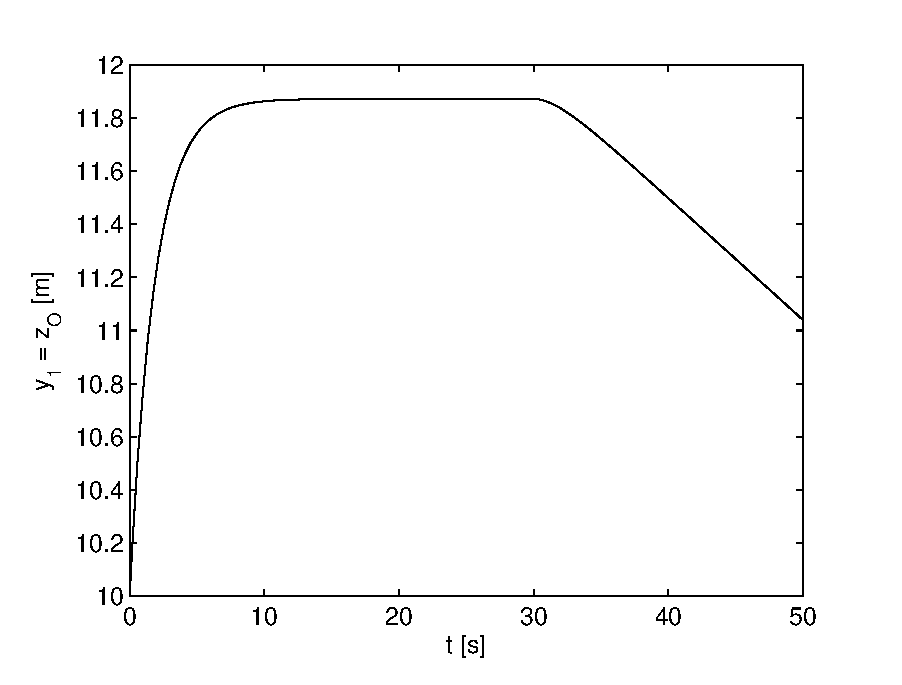
\includegraphics[width=0.34\textwidth]{Figs/zlanl}\label{zlanl}}
\subfigure[]{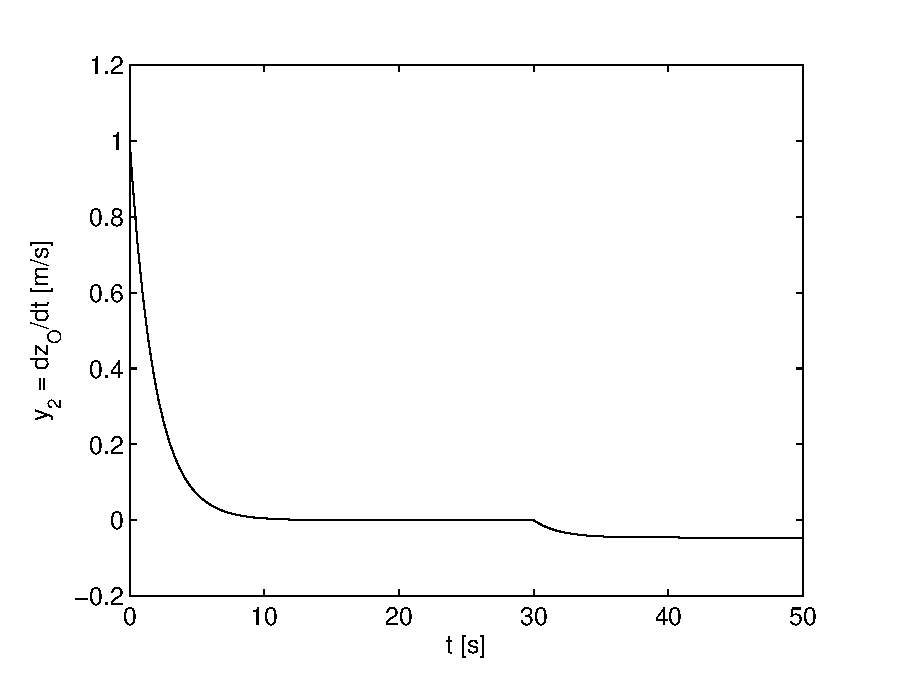
\includegraphics[width=0.34\textwidth]{Figs/dzlanl}\label{dzlanl}}
\subfigure[]{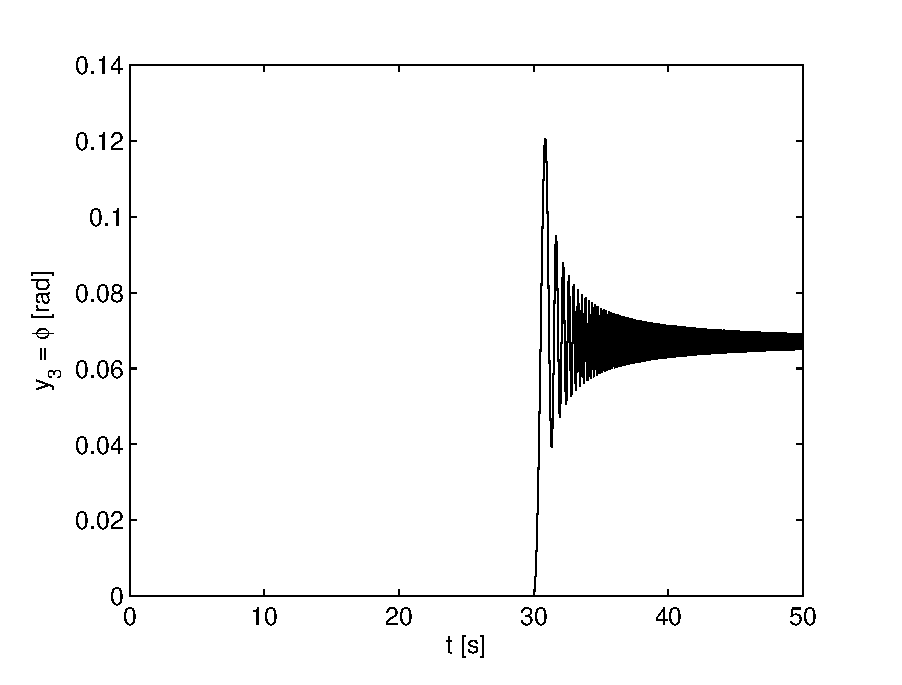
\includegraphics[width=0.34\textwidth]{Figs/philanl}\label{philanl}}
\subfigure[]{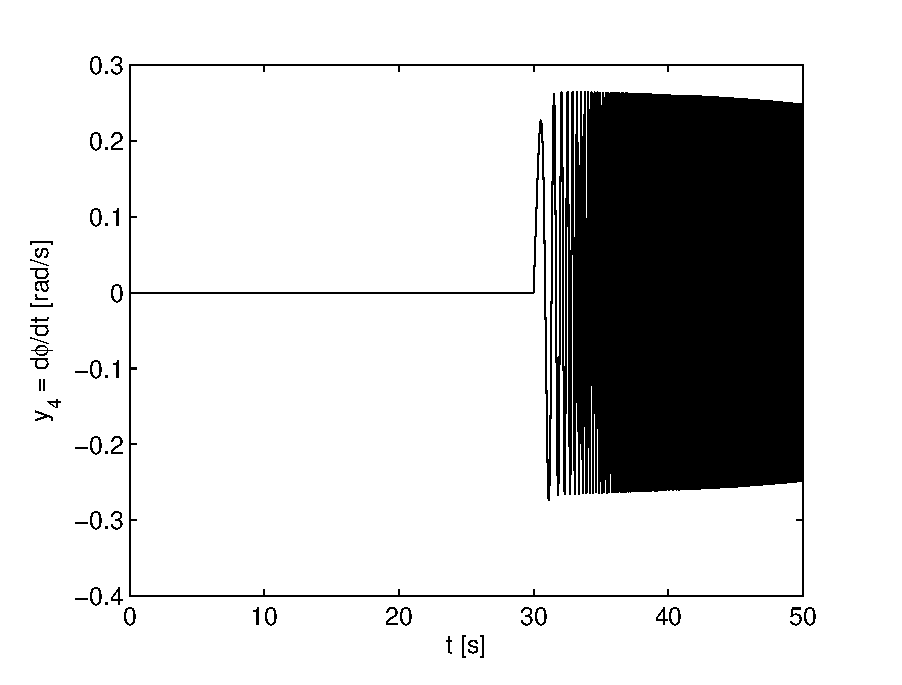
\includegraphics[width=0.34\textwidth]{Figs/dphilanl}\label{dphilanl}}
\subfigure[]{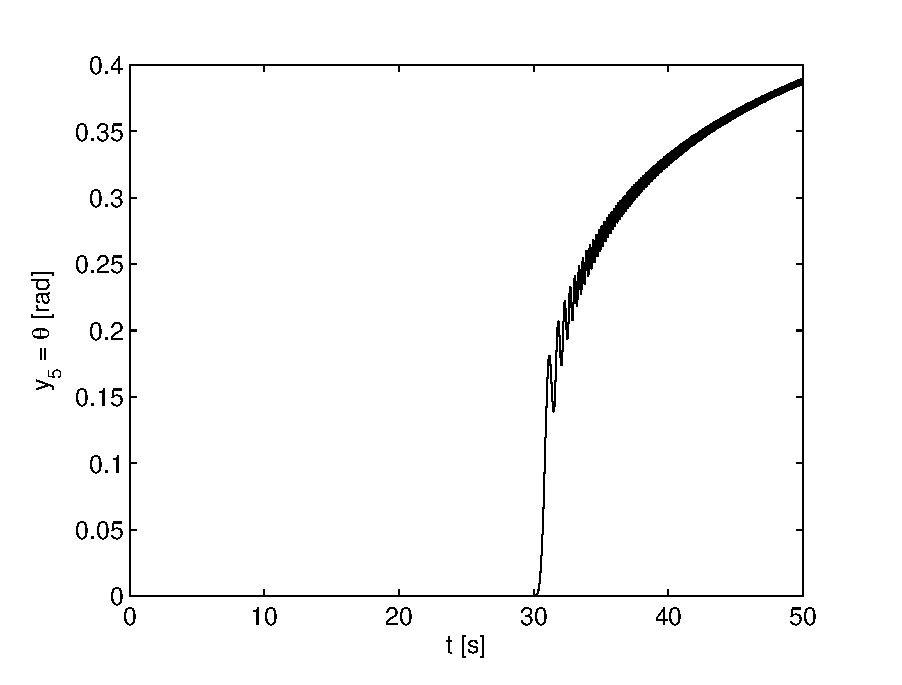
\includegraphics[width=0.34\textwidth]{Figs/thetalanl}\label{thetalanl}}
\subfigure[]{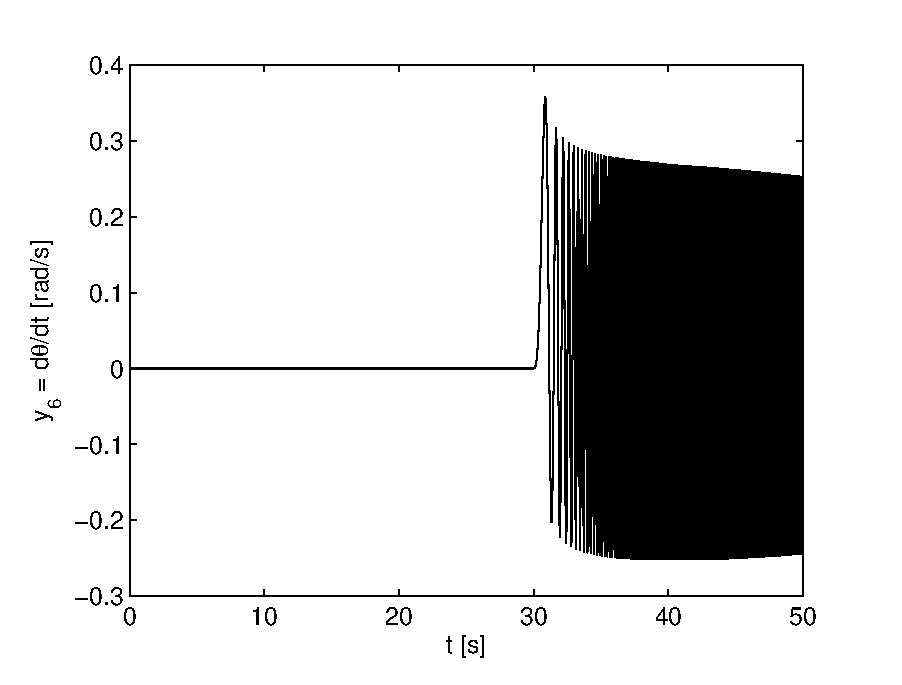
\includegraphics[width=0.34\textwidth]{Figs/dthetalanl}\label{dthetalanl}}
\subfigure[]{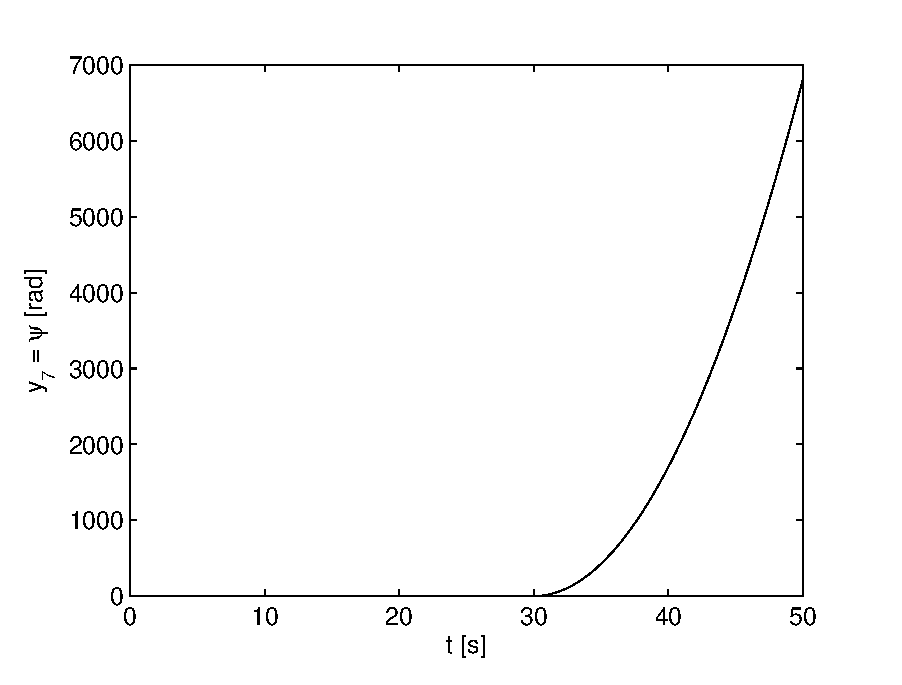
\includegraphics[width=0.34\textwidth]{Figs/psilanl}\label{psilanl}}
\subfigure[]{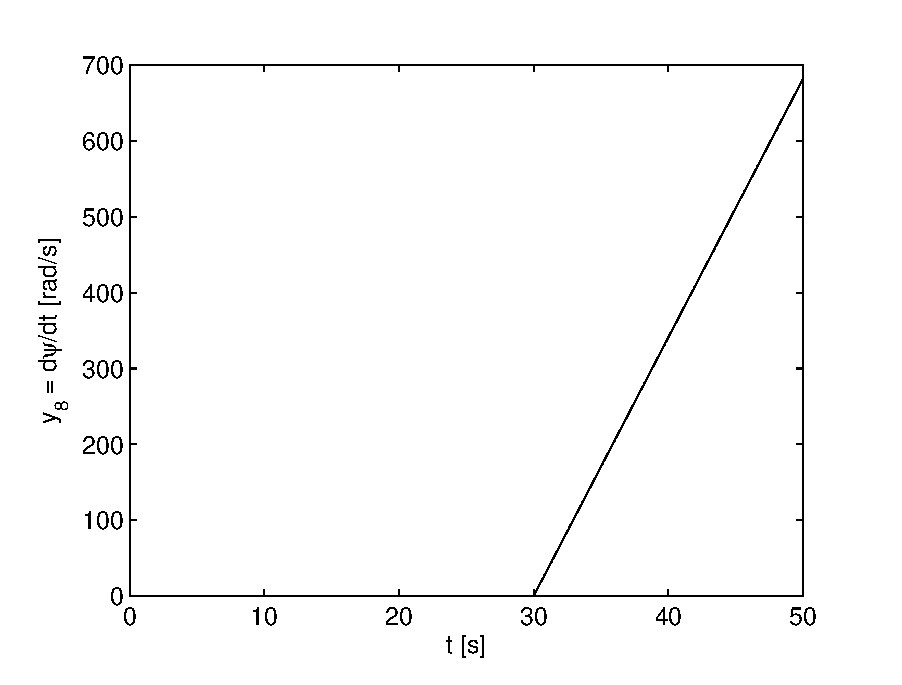
\includegraphics[width=0.34\textwidth]{Figs/dpsilanl}\label{dpsilanl}}
\caption[Simulaci�n equilibrio perturbado]{Simulaci�n del sistema ante condiciones de equilibrio perturbado: (a) $z(t)$, (b) $\dot{z}(t)$, (c) $\phi(t)$, (d) $\dot{\phi}(t)$, (e) $\theta(t)$, (f) $\dot{\theta}(t)$, (g) $\psi(t)$ y (h) $\dot{\psi}(t)$}\label{lanl}
\end{figure}
% ------------------------------------------------------------------------
\begin{figure}
\centering
\subfigure[]{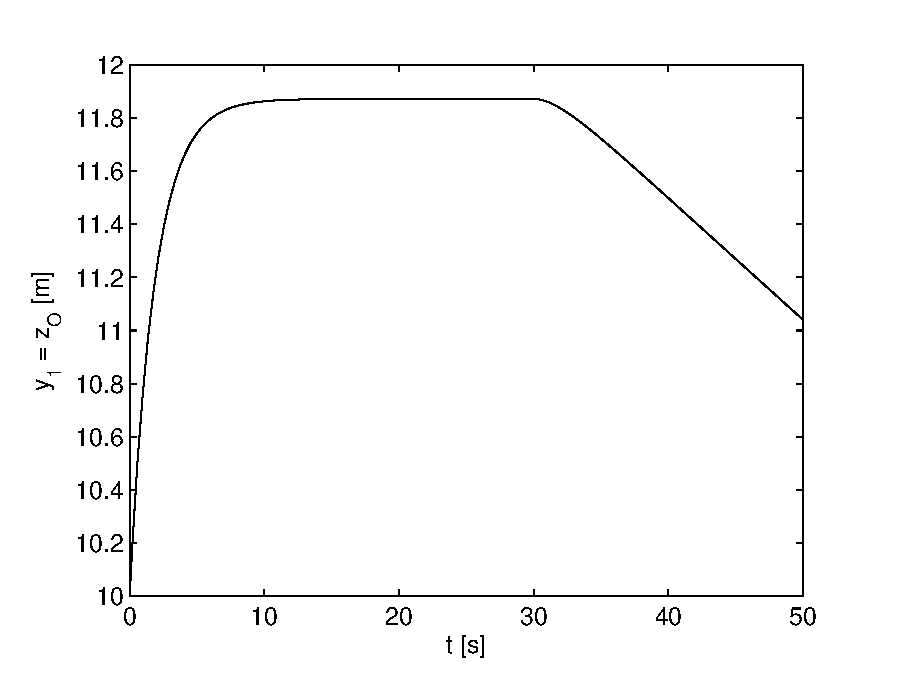
\includegraphics[width=0.34\textwidth]{Figs/zlanl2}\label{zlanl2}}
\subfigure[]{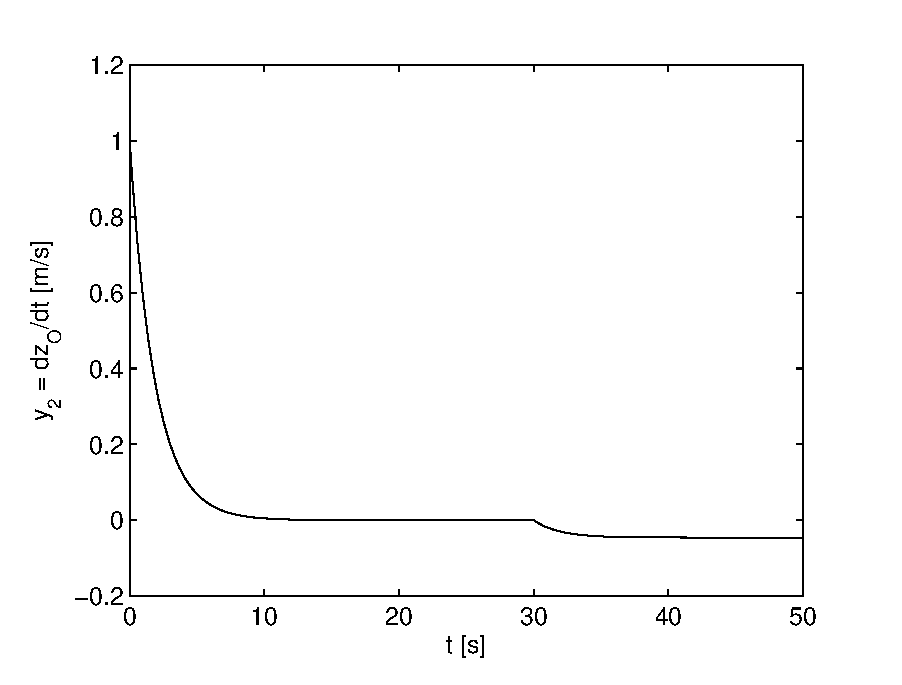
\includegraphics[width=0.34\textwidth]{Figs/dzlanl2}\label{dzlanl2}}
\subfigure[]{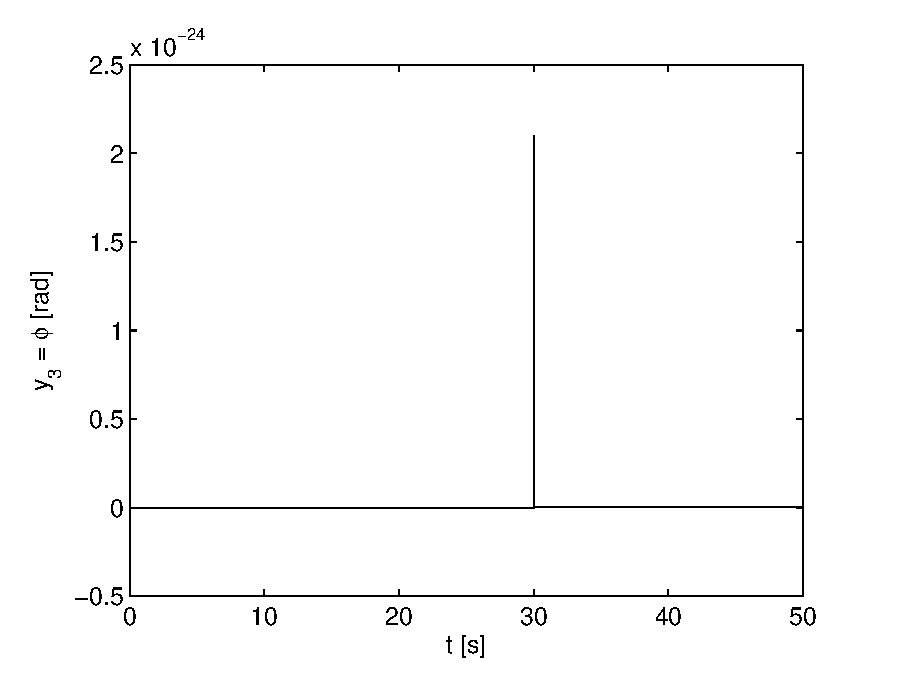
\includegraphics[width=0.34\textwidth]{Figs/philanl2}\label{philanl2}}
\subfigure[]{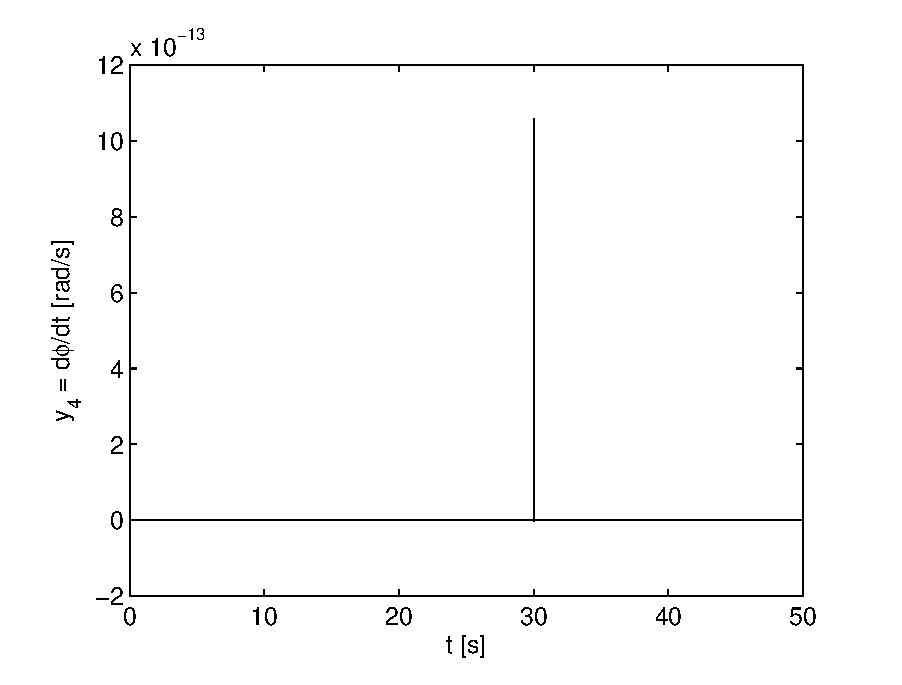
\includegraphics[width=0.34\textwidth]{Figs/dphilanl2}\label{dphilanl2}}
\subfigure[]{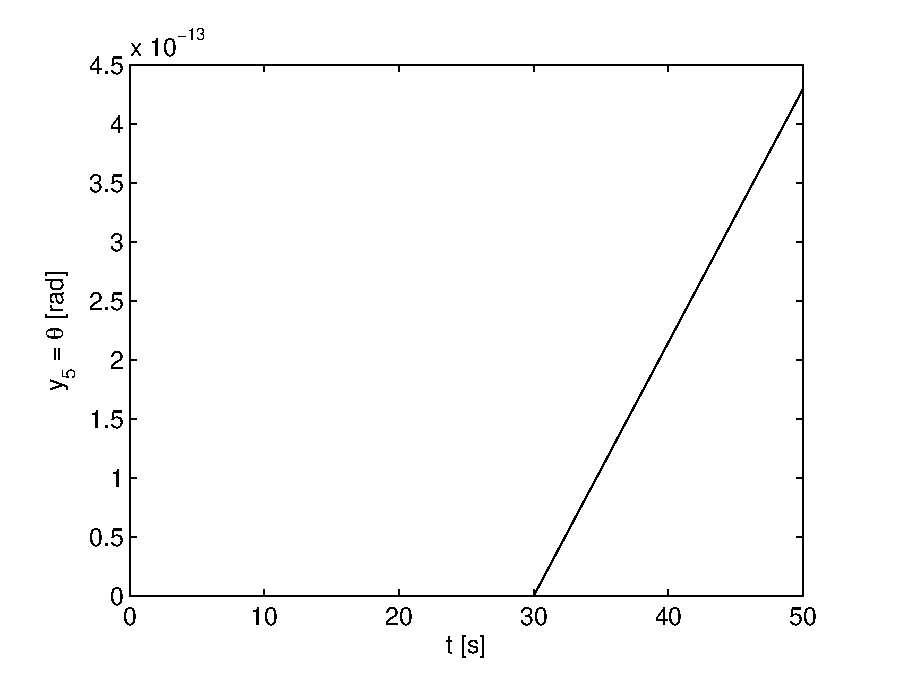
\includegraphics[width=0.34\textwidth]{Figs/thetalanl2}\label{thetalanl2}}
\subfigure[]{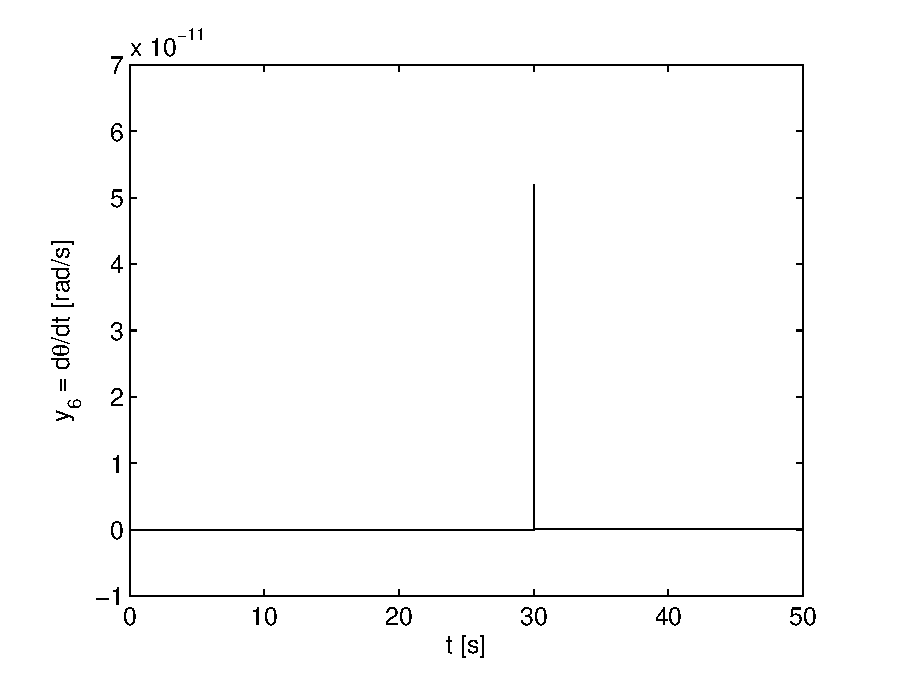
\includegraphics[width=0.34\textwidth]{Figs/dthetalanl2}\label{dthetalanl2}}
\subfigure[]{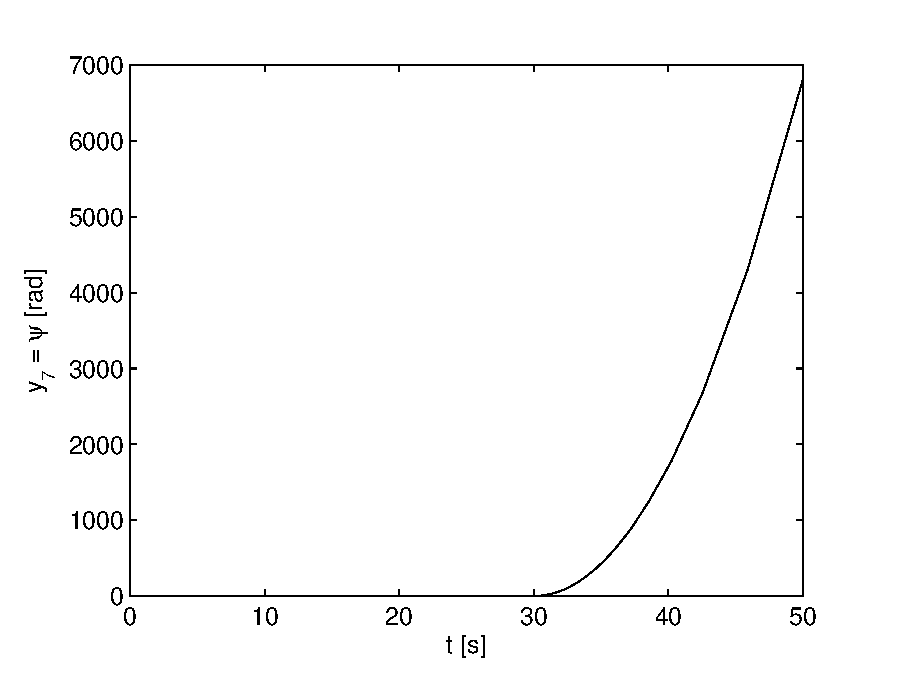
\includegraphics[width=0.34\textwidth]{Figs/psilanl2}\label{psilanl2}}
\subfigure[]{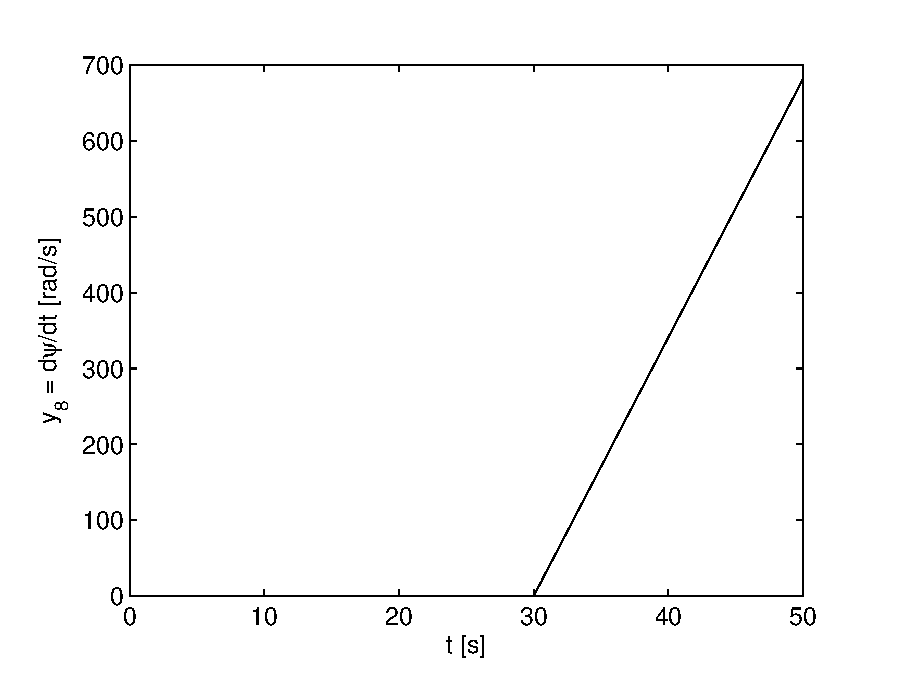
\includegraphics[width=0.34\textwidth]{Figs/dpsilanl2}\label{dpsilanl2}}
\caption[Simulaci�n equilibrio perturbado con fricci�n]{Simulaci�n del sistema ante condiciones de equilibrio perturbado con efecto girosc�pico: (a) $z(t)$, (b) $\dot{z}(t)$, (c) $\phi(t)$, (d) $\dot{\phi}(t)$, (e) $\theta(t)$, (f) $\dot{\theta}(t)$, (g) $\psi(t)$ y (h) $\dot{\psi}(t)$}\label{lanl2}
\end{figure}
%----------------------------------------------------------------------------------------------------------------
%----------------------------------------------------------------------------------------------------------------
%----------------------------------------------------------------------------------------------------------------
%----------------------------------------------------------------------------------------------------------------
%----------------------------------------------------------------------------------------------------------------    % Modelo matem�tico del DRON
% ------------------------------------------------------------------------
% ------------------------------------------------------------------------
% ------------------------------------------------------------------------
%                                Cap�tulo 4
% ------------------------------------------------------------------------
% ------------------------------------------------------------------------
% ------------------------------------------------------------------------

\chapter{Controladores PI y su conjunto estabilizante}
% ------------------------------------------------------------------------.
\noindent Como complemento a los desarrollos presentados en el cap�tulo anterior, se analiza a continuaci�n
la incidencia de conjuntos estabilizantes en controladores cl�sicos del tipo proporcional/integral (m�s conocidos como PI),
sintonizados empleando las reglas de \emph{Ziegler \& Nichols}. La manera de abordar el problema involucra una revisi�n general de conceptos, el c�lculo de $\mathcal{S}$ para un caso de estudio y la definici�n de una m�trica para valorar la \emph{fragilidad} del controlador dise�ado.
% ------------------------------------------------------------------------
% ------------------------------------------------------------------------
% ------------------------------------------------------------------------
\section{Controladores PID}
% ------------------------------------------------------------------------
\noindent La acci�n de control proporcional/integral/derivativo (o simplemente PID), constituye la estrategia de control m�s empleada en automatizaci�n de procesos industriales \citep{Astrom1995}.\\

Entre las razones por las cuales se prefiere el uso de controladores PID, se incluye la simplicidad de su estructura que con tan s�lo 3 t�rminos permite asegurar rechazo ante perturbaciones, velocidades de respuesta apropiadas y la eliminaci�n de errores en estado estacionario. Lo anterior, facilita el c�lculo de par�metros de control al igual que su operaci�n y mantenimiento \citep{Diaz2016} \citep{Diaz2017} \citep{Mendez2008}.\\

Fundamentalmente, la estructura de una acci�n PID est� constituida de una parte \emph{proporcional al error}:
$$
u_P = k_{P}e(t),
$$\
siendo $e(t)$ el error de medida y $k_P$ la ganancia proporcional; una parte \emph{proporcional a la historia
del error} (a partir del operador de memoria integral en el tiempo):
$$
u_I = k_{I}\int_{0}^{t}{e(t)dt},
$$
con ganancia integral $k_I$ y finalmente, una parte \emph{proporcional al cambio reciente del error} (a partir del operador anticipativo derivada temporal):
$$
u_D = k_{D}\frac{d}{dt}e(t),
$$
con ganancia derivativa $k_D$. La superposici�n de las tres acciones anteriores permite constituir la siguiente expresi�n para el esfuerzo de control:
% ------------------------------------------------------------------------
\begin{eqnarray}
u_{PID}(t) & = & u_P + u_I + u_D \\
           & = & k_{P}e(t) + k_I\int_{0}^{t}{e(t)dt} + k_{D}\frac{d}{dt}e(t) \\
           & = & k_P \left( e(t) + \frac{1}{T_I}\int_{0}^{t}{e(t)dt} + T_D \frac{d}{dt}e(t) \right),
\end{eqnarray}\
% ------------------------------------------------------------------------
siendo $T_I$ el tiempo integral y $T_D$ el tiempo derivativo. El esquema general para la realizaci�n de un controlador PID en forma paralela, se presenta en la Fig. \ref{PID_Diag}.\\
% ------------------------------------------------------------------------
\begin{figure}[h]
\centering
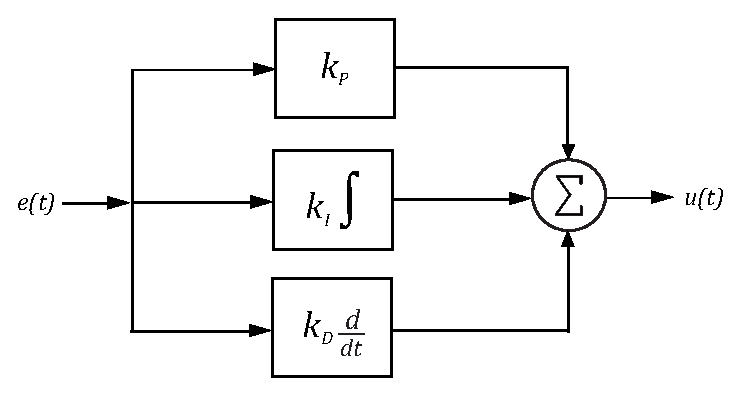
\includegraphics[width=0.5\textwidth]{figs/PID_Diagrama}
\caption{Controlador PID en forma de realizaci�n paralela}\label{PID_Diag}
\end{figure}
% ------------------------------------------------------------------------

% ------------------------------------------------------------------------
\subsection{Reglas de sintonizaci�n}
% ------------------------------------------------------------------------
\noindent La determinaci�n de los par�metros del controlador ($k_P$, $T_I$ y $T_D$), que satisfagan condiciones deseadas de desempe�o para el sistema controlado, se denomina \emph{procedimiento de sintonizaci�n}.\\

Existen fundamentalmente dos grandes tipos de m�todos de dise�o o sintonizaci�n de controladores PID: \emph{1)} los \emph{m�todos anal�ticos} basados en el modelo y \emph{2)} los \emph{m�todos emp�ricos} o experimentales basados en datos reales del proceso.\\

Dentro del primer grupo, se encuentran los m�todos cl�sicos en el dominio de la frecuencia como el lugar de las ra�ces o la respuesta en frecuencia mediante diagramas de \emph{Bode} y de \emph{Nyquist}. Sin embargo, estos m�todos requieren el conocimiento de un modelo matem�tico suficientemente apropiado para la din�mica de la planta.\\

En ocasiones sin embargo este modelo de la planta no se encuentra disponible o simplemente su determinaci�n es inviable, por ejemplo por falta de informaci�n de la constituci�n interna del sistema. Ante esta situaci�n los m�todos de control basados en datos (\emph{data-driven control} \citep{Safonov1997}) adquieren particular relevancia.\\

A nivel de t�cnicas de sintonizaci�n de controladores PID basadas en datos se destaca el trabajo cl�sico desarrollado por \emph{Ziegler \& Nichols} en 1942 \citep{Ziegler1942}, el cu�l ha sido la base hasta nuestros d�as de m�todos de sintonizaci�n para controladores que operan en aplicaciones industriales de diferente naturaleza.\\

M�todos adicionales de sintonizaci�n para controladores PID incluyen: el de \emph{sintonizaci�n de rel�} \citep{Diaz2017}; el \emph{Cohen-Coon} \citep{Alfaro2002} y otros m�s modernos involucrando optimizaci�n de m�rgenes de estabilidad a partir de herramientas computacionales \citep{Alzate2016} \citep{Diaz2016} \citep{Fung1998} \citep{Hang1992} \citep{toscano2005}.\\

Para una revisi�n detallada de m�todos de sintonizaci�n para controladores PID, se recomienda al lector interesado consultar \citep{Correa2008}.

% ------------------------------------------------------------------------
\section{An�lisis de estabilidad para un controlador PI}\label{estabanalpi}
% ------------------------------------------------------------------------
\noindent A pesar que un controlador PID concentra en una misma estructura las acciones de control necesarias para asegurar una forma de onda adecuada en la respuesta del sistema controlado, la acci�n derivativa se considera nociva en t�rminos de amplificaci�n de ruidos.\\

Por esta raz�n, el controlador proporcional/integral o simplemente PI es una estructura todav�a m�s simple, que concentra los mayores beneficios de simpleza y utilidad pr�ctica en aplicaciones. La funci�n de transferencia para un controlador PI (o PID con acci�n derivativa nula) viene dada por:
% -----------------------------------------------------------------------
\begin{eqnarray}
\nonumber C(s) & = & k_P \left( 1 + \frac{1}{T_I s}\right)\\
               & = & \frac{k_Ps + k_I}{s}.\label{PIconteq}
\end{eqnarray}\

% ------------------------------------------------------------------------
\subsection{Sintonizaci�n PI por \emph{Ziegler \& Nichols}}
% -----------------------------------------------------------------------
\noindent Considere el sistema dado por:
% ------------------------------------------------------------------------
\begin{equation}
P(s)=\frac{N(s)}{D(s)}=\frac{1}{s(s+1)(s+5)},\label{plantaCPI}
\end{equation}\
% ------------------------------------------------------------------------
y proceda a calcular los par�metros de un controlador PI para el mismo empleando las reglas de \emph{Ziegler \& Nichols}.\\

Inicialmente, se recuerda que existen dos posibles m�todos \citep{ogata2010}:
% ------------------------------------------------------------------------
\begin{itemize}
% ------------------------------------------------------------------------
\item[-] \emph{Lazo cerrado:} donde para una acci�n proporcional pura en el sistema realimentado, se aplican cambios de tipo escal�n en la referencia
buscando identificar el valor de $k_P$ para el cual el sistema oscila con amplitud sostenida. Este valor de ganancia se denomina ganancia cr�tica $k_{cr}$ y al periodo de oscilaci�n correspondiente periodo cr�tico $P_{cr}$;
\item[-] \emph{Lazo abierto:} cuando no existe un valor $k_{cr}$ que produzca oscilaciones sostenidas, se recurre a aplicar un est�mulo de tipo escal�n al sistema en lazo abierto buscando obtener una respuesta en forma de \emph{s} tal y como la ilustrada en la Fig. \ref{ZNol}, siendo \emph{T} y \emph{L} las cantidades a ser tomadas en cuenta.
% ------------------------------------------------------------------------
\end{itemize}
% ------------------------------------------------------------------------
\begin{figure}[h]
\centering
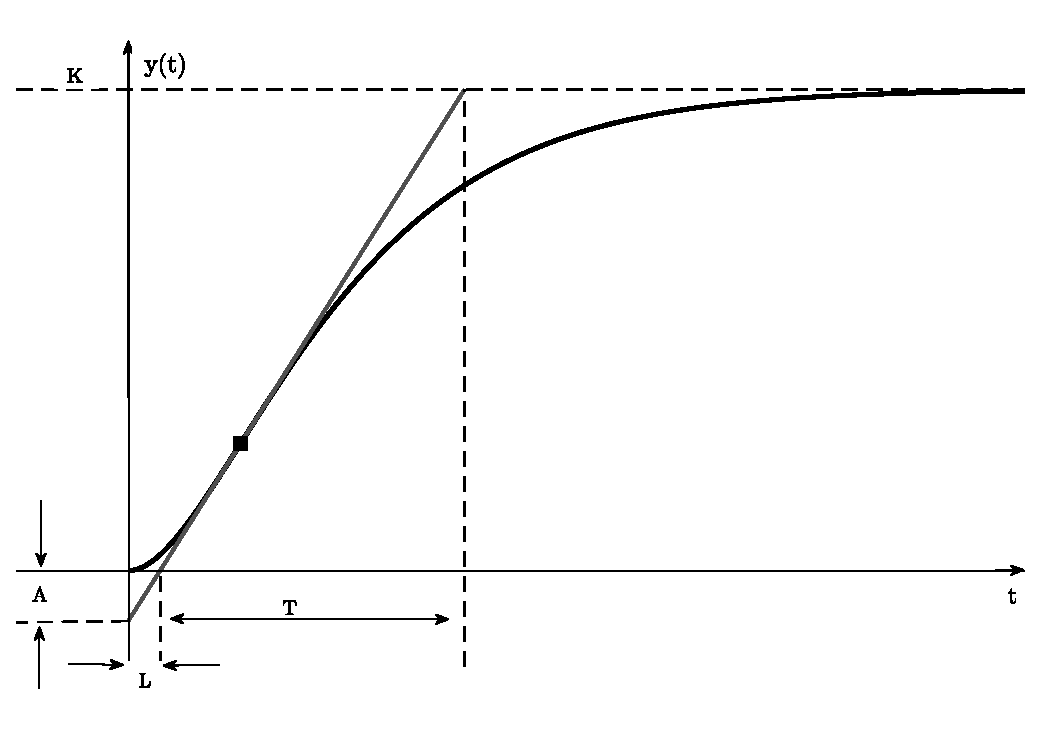
\includegraphics[width=0.5\textwidth]{figs/ZNol}
\caption{Respuesta escal�n en forma de \emph{s} del m�todo en lazo abierto}\label{ZNol}
\end{figure}
% ------------------------------------------------------------------------
Una vez obtenidos los valores importantes para cada caso, los par�metros del controlador PI (i.e. ganancia proporcional $k_P$ y tiempo integral $T_I$) se determinan con base en las equivalencias presentadas en la Tabla \ref{table_PI}.\\

% ------------------------------------------------------------------------
\begin{table}[htbp]
\caption[C�lculo controlador PI m�todos de \emph{Ziegler \& Nichols}]{Equivalencias c�lculo controlador PI para m�todos de \emph{Ziegler \& Nichols}}\label{table_PI}
	\centering
    \begin{threeparttable}
	\begin{tabular}{ c  c  c }
    \hline
    M�todo                       & $k_P$               & $T_I$                  \\ \hline
    \multicolumn{1}{c}{Lazo abierto}      & $0.45k_{cr}$        & $\frac{1}{1.2}P_{cr}$  \\
    \multicolumn{1}{c}{Lazo cerrado}      & $0.9 \frac{T}{L}$   & $\frac{L}{0.3}$        \\ \hline
	\end{tabular}
% ------------------------------------------------------------------------
\begin{tablenotes}
\scriptsize
\item[ ] \emph{Nota:} Adaptado de \citep{ogata2010}.
\end{tablenotes}
% ------------------------------------------------------------------------
\end{threeparttable}
\end{table}
% ------------------------------------------------------------------------

En el caso particular de una configuraci�n realimentada como la presentada en la Fig. \ref{sistem2ord} para la combinaci�n de planta y controlador dada respectivamente por las expresiones \eqref{plantaCPI} y \eqref{PIconteq}, es posible mostrar que el lugar geom�trico de las ra�ces para el sistema realimentado cruza el eje imaginario cuando $k_P = k_{cr} = 30$, con oscilaciones sostenidas de periodo $P_{cr} = 2.81 \: [s]$.\\

De esta manera, el controlador dise�ado corresponde con $k_P = 13.50$; $T_I = 2.34$; es decir:
% ------------------------------------------------------------------------
\begin{eqnarray}
\nonumber C(s) & = & 13.50 \left( 1 + \frac{1}{2.34 s}\right)\\
               & = & \frac{13.50s + 5.76}{s}
               \label{PIconteqval}.
\end{eqnarray}\
% ------------------------------------------------------------------------

Los par�metros de respuesta para el sistema compensado empleando dicho controlador, corresponden con:
$$
Mp = 104.05 \: [\%]; \quad t_s = 249.54 \: [s],
$$

seg�n ilustrado en la respuesta escal�n de la Fig. \ref{step_PI}.\\

Esta respuesta din�mica a pesar de ser estable, no representa un resultado
satisfactorio en t�rminos de velocidad de convergencia hacia el valor de estado estacionario, dadas las evidentes oscilaciones del r�gimen transitorio y el prolongado tiempo de establecimiento. Dicha condici�n es susceptible de mejora a trav�s de un \emph{ajuste fino}. N�tese sin embargo, que la acci�n de control es simple (PI) y la planta es de un orden significativo (tercero).\\

% ------------------------------------------------------------------------
\begin{figure}[h]
\centering
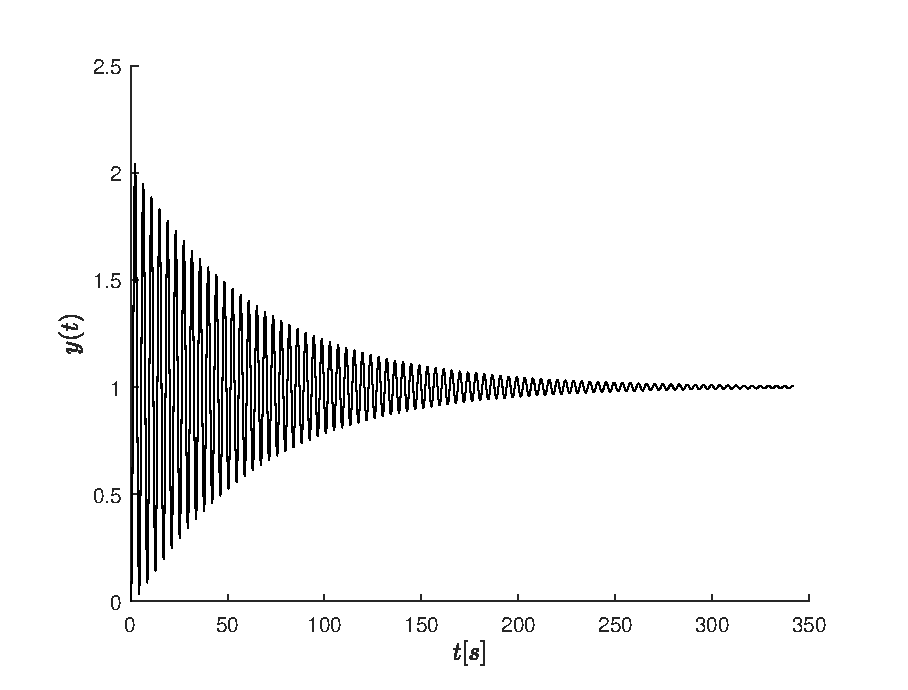
\includegraphics[width=0.5\textwidth]{figs/step_PI}
\caption{Respuesta escal�n del sistema compensado}\label{step_PI}	
\end{figure}

% ------------------------------------------------------------------------
\subsection{Conjunto estabilizante para sistema ante control PI}\label{conjestabpi}
% ------------------------------------------------------------------------
\noindent Empleando un tratamiento similar al utilizado para el an�lisis del conjunto estabilizante de la \emph{Secci�n} \ref{estabsect}, es posible deducir que la combinaci�n de planta + controlador definida en \eqref{plantaCPI} y \eqref{PIconteq}, permite delimitar una regi�n de estabilidad en el plano ($k_P$, $k_I$) dada por:
% ------------------------------------------------------------------------
\begin{eqnarray}
0 & < & k_{P} < 30; \label{stabsetPI1} \\
0 & < & k_{I} < \frac{-k_{P}^{2}+30k_{P}}{36},\label{stabsetPI2}
\end{eqnarray}
% ------------------------------------------------------------------------
definiendo a su vez el siguiente conjunto estabilizante:
\begin{equation}
\mathcal{S} = \left\{\left(k_P, k_I\right): \: \text{\eqref{stabsetPI1} y \eqref{stabsetPI2} se satisfagan simult�neamente} \right\}.\label{stabsetPIeq}
\end{equation}
% ------------------------------------------------------------------------
La Fig. \ref{Stab_set_PI} ilustra el conjunto estabilizante \eqref{stabsetPIeq}, resaltando en su interior mediante un asterisco el punto correspondiente al controlador dise�ado y definido en \eqref{PIconteqval}.\\
% ------------------------------------------------------------------------
\begin{figure}[h]
\centering
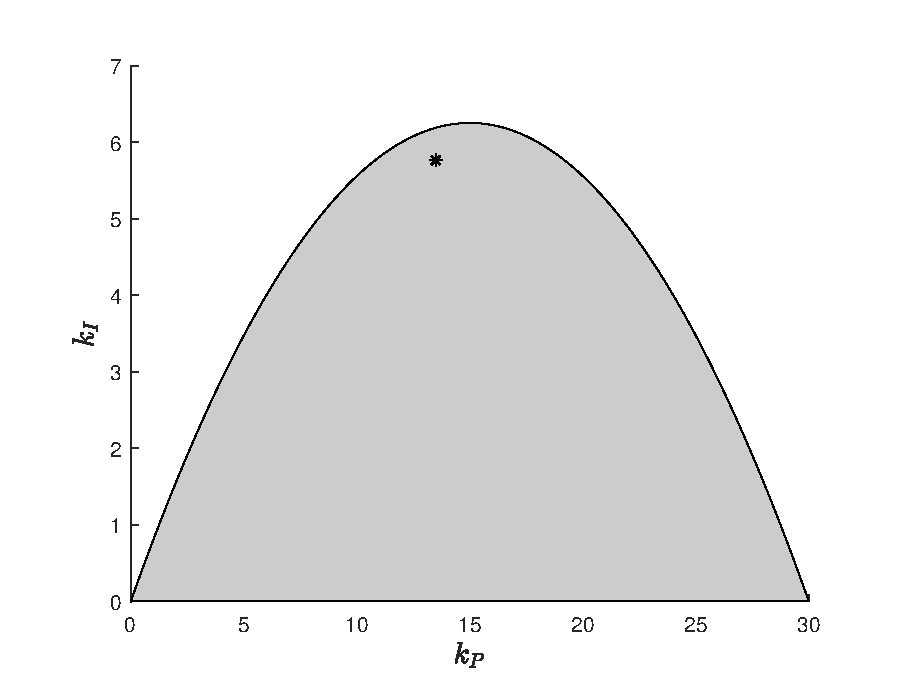
\includegraphics[width=0.5\textwidth]{figs/stab_set_PI}
\caption{Conjunto estabilizante en el plano ($k_P$, $k_I$)}\label{Stab_set_PI}
\end{figure}
% ------------------------------------------------------------------------

Como se observa, el controlador analizado en la Fig.\ref{step_PI} se encuentra cerca de los l�mites de estabilidad, justificando la alta oscilaci�n de su respuesta din�mica.\\

La siguiente \emph{Secci�n} realizar� un an�lisis alrededor de la \emph{fragilidad} del controlador PI.

% ------------------------------------------------------------------------
\section{Fragilidad de controladores PI}
% ------------------------------------------------------------------------
\noindent Los m�todos de \emph{Ziegler \& Nichols} para la sintonizaci�n de controladores PI y PID
han sido la referencia empleada por ingenieros en diversos campos de aplicaci�n desde su
aparici�n en 1942. Sin embargo, como se observ� en el ejemplo presentado en la \emph{Secci�n} anterior, no siempre se logra una respuesta din�mica adecuada a las exigencias
de una respuesta deseada, aunque la misma sea estable.\\

La forma tradicional de corregir esta situaci�n, es considerar que los par�metros del
controlador PI o PID obtenidos por el m�todo de \emph{Ziegler \& Nichols} son el valor inicial
de un proceso iterativo denominado \emph{ajuste fino}, que permitir� eventualmente obtener
una respuesta mejorada en t�rminos de \emph{nuevos valores sintonizados}.\\

El objetivo de la presente \emph{Secci�n} no es discutir el proceso de sinton�a fina de par�metros en los m�todos de Ziegler \& Nichols, sino evaluar la \emph{fragilidad del controlador} dise�ado con dicho m�todo, en t�rminos
de su conjunto estabilizante.\\

En \citep{Bhatt97} Bhattacharyya define la \emph{fragilidad de un controlador} como aquel fen�meno que implica para el mismo m�rgenes de estabilidad extremadamente peque�os. Otra manera de entender el concepto es a trav�s de la m�s peque�a perturbaci�n admisible en los par�metros de un controlador tal que el sistema realimentado pierda su estabilidad. La fragilidad es un concepto muy cercano a la robustez, y  por tanto conviene enfatizar en que la primera estudia la manera en que alteraciones leves en los valores de par�metro de un controlador afectan la estabilidad del sistema realimentado, mientras que la segunda realiza el estudio independientemente de donde hayan ocurrido las variaciones param�tricas.

% ------------------------------------------------------------------------
\subsection{Geometr�a para m�rgenes de estabilidad en un controlador PI}\label{margeom}
% ------------------------------------------------------------------------
\noindent Una interpretaci�n geom�trica del margen de fase para un sistema
realimentado ante un control PI, se propone en \citep{Alzate2016}. El desarrollo presentado en el presente numeral se basa en el trabajo referenciado
y sugiere la manera de aplicar el mismo resultado en t�rminos del margen de ganancia del sistema.\\

Para ello, asuma $P(j\omega)$ y $C(j\omega)$ como la respuesta frecuencial de la planta y el controlador PI definidos en \eqref{plantaCPI} y \eqref{PIconteq}, respectivamente. En el sistema realimentado estable que se obtiene a partir de esta combinaci�n \emph{planta + controlador}, los m�rgenes de ganancia $A_m$ y fase $\theta_m$ se pueden determinar anal�ticamente a partir de las condiciones de magnitud y fase:
% ------------------------------------------------------------------------
\begin{equation}
 |P(j\omega_g)||C(j\omega_g)| =1, \label{CondMag}
\end{equation}
% ------------------------------------------------------------------------
% ------------------------------------------------------------------------
\begin{equation}
\angle{P(j\omega_{\theta})}+\angle{C(j\omega_{\theta})}={\pi}n; \quad n=\pm 1,3,5... \label{Condpha}
\end{equation}
% ------------------------------------------------------------------------
de manera que:
% ------------------------------------------------------------------------
\begin{equation}
A_m=\frac{1}{|P(j\omega_{\theta})||C(j\omega_{\theta})|}, \label{Am}
\end{equation}
% ------------------------------------------------------------------------
% ------------------------------------------------------------------------
\begin{equation}
\theta_m=\angle{P(j\omega_{g})}+\angle{C(j\omega_{g})}-\pi, \label{pm}
\end{equation}
% ------------------------------------------------------------------------
siendo $w_g$ y $w_{\theta}$ las frecuencias de cruce de ganancia y fase, respectivamente.\\

Alternativamente, estos margenes de estabilidad pueden obtenerse a partir de una relaci�n geom�trica en el plano de par�metros $\left(k_P, k_I\right)$ de un controlador PI, con respecto al conjunto estabilizante $\mathcal{S}$ de la planta bajo esta acci�n de control.\\

As� entonces, tomando en cuenta que:
% -----------------------------------------------------------------------
\begin{eqnarray}
\nonumber C(j \omega) & = & k_P + \frac{k_I}{j \omega}\\
                      & = & k_P - \frac{k_I}{\omega}j,
\end{eqnarray}
% -----------------------------------------------------------------------
la fase del controlador PI puede expresarse como:
% ------------------------------------------------------------------------
\begin{eqnarray}
\angle{C(j\omega)} & = & \arctan{\left(\frac{-k_I}{{\omega}k_P}\right)} \label{phi_c},
\end{eqnarray}
% ------------------------------------------------------------------------
o equivalentemente:
% ------------------------------------------------------------------------
\begin{eqnarray}
-\omega{k_P}\tan\left(\angle{C(j\omega)}\right) & = & k_I. \label{recta}
\end{eqnarray}\
% ------------------------------------------------------------------------

Si en la expresi�n anterior se asume $\omega = \omega_g$, la fase del controlador $\angle{C(j\omega_{g})}$ debe satisfacer un margen de fase $\theta_m$ ante una respuesta frecuencial $P(j \omega)$ conocida para la planta, seg�n definido en \eqref{pm}. Por tanto, ante esta situaci�n la expresi�n \eqref{recta} define una linea recta en el plano $\left(k_P, k_I\right)$ con pendiente $-\omega{\tan\left(\angle{C(j\omega)}\right)}$, cuyos puntos satisfacen dichas restricciones.\\

Asimismo, a partir de la condici�n de magnitud del controlador se tiene:
% ------------------------------------------------------------------------
\begin{eqnarray}
{|C(j\omega)|}^2 & = & {k_P}^{2}+\frac{{k_I}^{2}}{\omega^{2}}, \label{M_c^2}
\end{eqnarray}
% ------------------------------------------------------------------------
o equivalentemente:
% ------------------------------------------------------------------------
\begin{eqnarray}
\frac{{k_P}^{2}}{{|C(j\omega)|}^2}+\frac{{k_I}^{2}}{{|C(j\omega)|}^2{\omega}^2} & = & 1. \label{elipse}
\end{eqnarray}\
% ------------------------------------------------------------------------

Bajo la misma suposici�n de $\omega = \omega_g$, la expresi�n anterior representar� una elipse en el plano $\left(k_P, k_I\right)$, que intersecta a la recta \eqref{recta} seg�n ilustrado en el diagrama de la Fig.~\ref{curvas1}.\\

El punto de intersecci�n, dar� la coordenada $\left(k_P, k_I\right)$ del controlador PI que satisface $\theta_m$ y $\omega_g$, representando un m�todo gr�fico para el dise�o de controladores.\\

Al respecto del m�todo se resaltan los siguientes detalles adicionales:
\begin{itemize}
\item[-] La intersecci�n entre la elipse y la linea recta se da para dos puntos del plano. Sin embargo, puede observarse de la Fig.~\ref{curvas1} que s�lo uno de ellos tiene sentido pr�ctico por encontrarse al interior del conjunto estabilizante $\mathcal{S}$;
\item[-] La magnitud para $C\left(j \omega_g\right)$ se deja como un par�metro libre de dise�o y de este depende la amplitud (i.e. radio mayor y radio menor) de la elipse en el plano;
\item[-] El margen de ganancia no se involucra expl�ticamente en el m�todo sugerido, aunque se entiende que la elecci�n arbitraria para $|C\left(j \omega_g\right)|$ influencia dicho valor. La Secci�n siguiente abordar� con mayor detalle este aspecto;
\item[-] El procedimiento sugerido puede abordarse expl�citamente desde el margen de ganancia, seleccionando $\omega = \omega_\theta$ y forzando de \eqref{Am} a la magnitud del controlador $|C(j\omega_{\theta})|$ a satisfacer un margen de ganancia $A_m$ ante una respuesta frecuencial $P(j \omega)$ conocida para la planta. Ante esta situaci�n, el punto de intersecci�n en el plano $\left( k_P, k_I \right)$ para la elipse y la linea recta representar� la coordenada $\left(k_P, k_I\right)$ del controlador PI que satisface $A_m$ y $\omega_\theta$, dejando como par�metro libre a la pendiente de la recta y a trav�s de ella, al margen de fase para el sistema controlado.
\end{itemize}
% ------------------------------------------------------------------------
\begin{figure}
\centering
	\subfigure[]{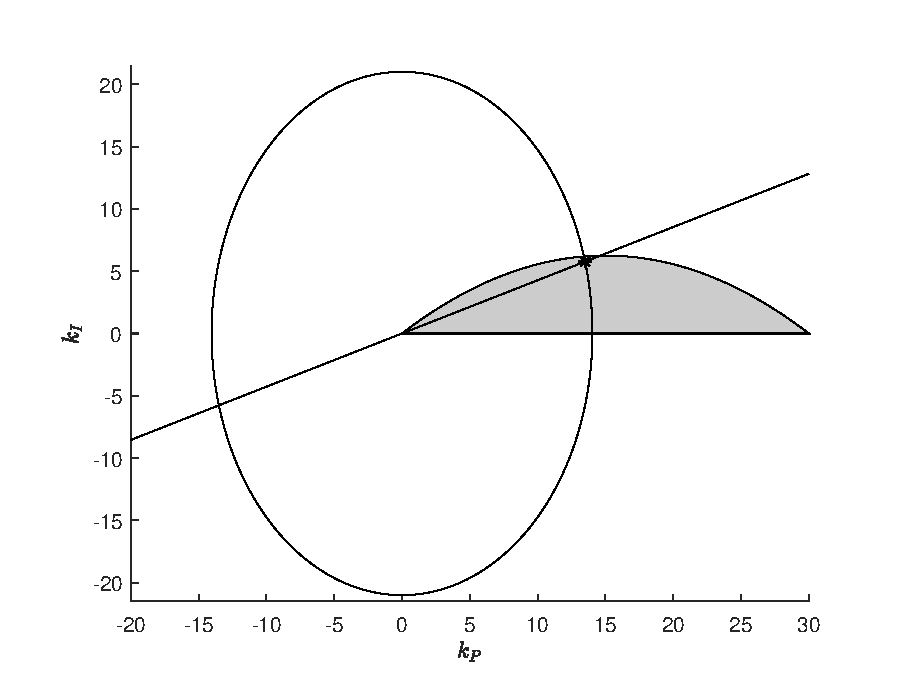
\includegraphics[width=0.5\textwidth]{Figs/curvas1}}
	\subfigure[]{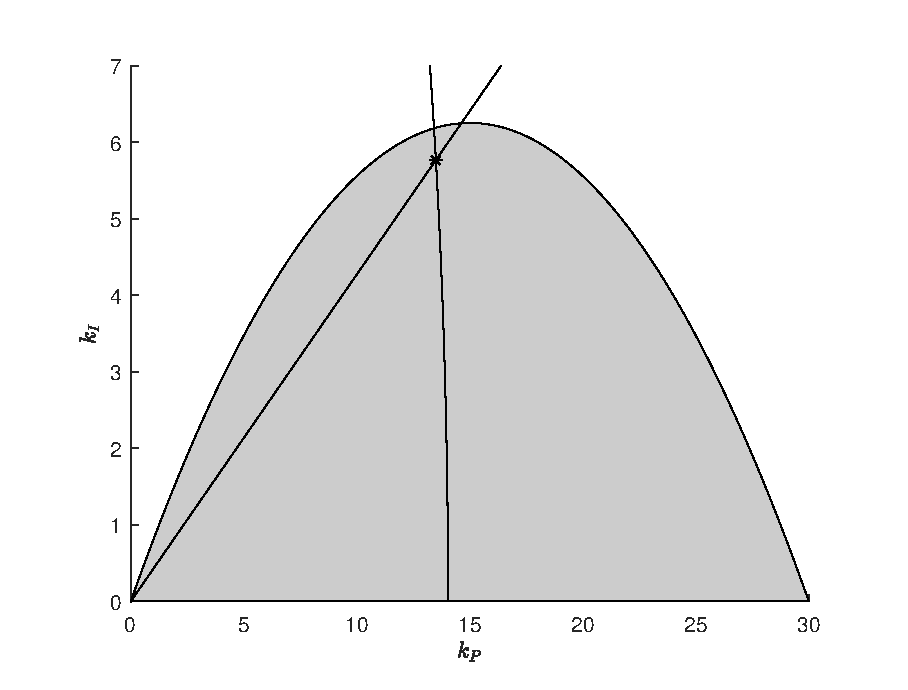
\includegraphics[width=0.5\textwidth]{Figs/curvas1-2}}
\caption[Intersecci�n en el plano $\left( k_P, k_I \right)$ para linea recta y elipse]{Intersecci�n en el plano $\left( k_P, k_I \right)$ para linea recta y elipse, dados $\omega = \omega_g$ y $\theta_m$, ilustrando: (a) panor�mica general de la intersecci�n y (b) detalle del punto de intersecci�n}\label{curvas1}
\end{figure}
% ------------------------------------------------------------------------

\subsection{Definici�n de m�trica para calcular distancia a inestabilidad}\label{metrdef}
% ------------------------------------------------------------------------
\noindent Como ya definido al principio de la presente \emph{Secci�n}, un buen dise�o para un controlador debe ir
m�s all� de la simple respuesta din�mica del sistema controlado y por tanto, debe adem�s garantizar
la estabilidad para el lazo de control a�n ante leves variaciones en sus
par�metros.\\

Complementando las ideas de \emph{Bhattacharyya y Keel} en \citep{Bhatt97}, se emplear� la visi�n geom�trica
propuesta por \emph{Morarescu et al} adaptada en el presente documento para
el caso de lazos PI sin retardo \citep{Mendez2008} \citep{Morarescu2010}.\\

Para ello, se define la distancia eucl�dea:
% ------------------------------------------------------------------------
\begin{equation}
d = \sqrt{(k_P^*-k_P)^2+(k_I^*-k_{I})^2},\label{d}
\end{equation}
% ------------------------------------------------------------------------
siendo $\left(k_P^*, k_I^* \right)$ las coordenadas para un controlador en el l�mite del conjunto estabilizante $\mathcal{S}$ y ortogonal a $\left(k_P, k_I \right)$, que define el radio para una circunferencia de puntos que representan un rango o margen de estabilidad.\\

A partir de lo anterior, dado un controlador PI al interior de $\mathcal{S}$ es posible cuantificar su \emph{fragilidad} a trav�s de esta m�trica, al menos en un modo relativo; es decir, dados dos controladores estables ser� m�s \emph{fr�gil} aquel para el cual se obtenga el menor $d$.\\

Sin embargo, no es claro el significado de \emph{fragilidad} para un valor $d$ en un contexto absoluto.\\

En cualquier caso, el c�lculo para $d$ en \eqref{d} implica conocer las coordenadas del punto $\left(k_P^*, k_I^* \right)$. Dichas coordenadas representan un valor en la frontera de $\mathcal{S}$, que conecta con el punto de an�lisis $\left(k_P, k_I \right)$ a trav�s de una l�nea recta y por tanto, en teor�a habr� una soluci�n para $\left(k_P^*, k_I^* \right)$ en cada direcci�n posible de proyecci�n para el vector $\left(k_P^*-k_P, k_I^*-k_I \right)$ en el plano. En \citep{Mendez2008} \citep{Morarescu2010} por ejemplo, los resultados presentados se realizan a partir de una proyecci�n sobre la vertical. Una soluci�n m�s general implica el m�nimo valor para $d$ en un barrido de $360�$ lo cual no es trivial, al menos anal�ticamente, si se piensa en que la descripci�n para la frontera de $\mathcal{S}$ corresponde con funciones definidas por tramos (es decir, con transiciones condicionadas).\\

Como alternativa, se presenta en el presente apartado una forma de calcular dicho punto l�mite a partir del enfoque geom�trico discutido en la \emph{Secci�n} \ref{margeom}. Para ello, considere el problema de cuantificar la fragilidad del controlador PI calculado en \eqref{PIconteqval}.\\

Dicho controlador representa un punto en el conjunto estabilizante $\mathcal{S}$ en \eqref{stabsetPIeq} y a su vez, la intersecci�n entre una l�nea recta y una elipse dadas respectivamente por \eqref{recta} y \eqref{elipse}, con los siguientes par�metros: $\omega_g = 1.49 \: rad/s$ y $\theta_m = 1.18�$ (el c�lculo para dichos par�metros fue realizado empleando la funci�n \emph{allmargins(.)} de MATLAB).\\

En t�rminos pr�cticos, la regla de dise�o indica que un buen margen de fase es alrededor de $60�$ \citep{Hang1992}. Como se observa el margen de fase $\theta_m$ obtenido por \emph{Ziegler \& Nichols} es muy cercano a la inestabilidad y por tanto sugiere \emph{fragilidad}.\\

Para determinar los valores l�mite $\left(k_P^*, k_I^* \right)$, se mantiene constante la pendiente de la recta \eqref{recta} a la misma frecuencia $\omega=\omega_g = 1.49 \: rad/s$ y se incrementa la amplitud de la elipse \eqref{elipse} a partir del par�metro $|C\left(j \omega_g\right)|$ (ver Fig.\ref{curvas2a}).\\

Ante estas condiciones, el margen de ganancia $A_m$ del sistema puede determinarse mediante el cociente entre las distancias eucl�deas correspondientes a los puntos $\left(k_P, k_I \right)$ y $\left(k_P^*, k_I^* \right)$; es decir \citep{Diaz2016}:
% ------------------------------------------------------------------------
\begin{eqnarray}
\nonumber A_m & = & \frac{\sqrt{\left(k_P^*\right)^2 + \left(k_I^*\right)^2}}{\sqrt{\left(k_P\right)^2 + \left(k_I\right)^2}}\\
\nonumber     & = & \frac{\sqrt{\left(k_P^*\right)^2 + \left(-\omega{k_P^*}\tan\left(\angle{C(j\omega)}\right)\right)^2}}{\sqrt{\left(k_P\right)^2 + \left(-\omega{k_P}\tan\left(\angle{C(j\omega)}\right)\right)^2}}\\
\nonumber     & = & \frac{k_P^*\sqrt{1 + \left(-\omega\tan\left(\angle{C(j\omega)}\right)\right)^2}}{k_P\sqrt{1 + \left(-\omega\tan\left(\angle{C(j\omega)}\right)\right)^2}}\\
\nonumber     & = & \frac{k_P^*}{k_P}\\
    & = & \frac{k_I^*}{k_I}.\label{margeng}
\end{eqnarray}\
% ------------------------------------------------------------------------

De este resultado se observa que si $\left(k_P, k_I \right)$ se encuentra en la frontera de $\mathcal{S}$ entonces $A_m = 1$; si $\left(k_P, k_I \right)$ se encuentra fuera  de $\mathcal{S}$ entonces $A_m < 1$ y si $\left(k_P, k_I \right)$ se encuentra dentro de $\mathcal{S}$ entonces $A_m > 1$, lo cual coincide con el comportamiento esperado
seg�n la teor�a para dicho margen en t�rminos de la estabilidad del sistema.\\

De esta manera, igualando \eqref{recta} para $k_I$ con la condici�n de frontera dada por \eqref{stabsetPI2}, se obtiene:
% ------------------------------------------------------------------------
\begin{eqnarray}
\nonumber -\omega_g {k_P^*}\tan\left(\angle{C(j\omega_g)}\right) & = & \frac{-\left(k_P^*\right)^{2}+30k_P^*}{36}\\
\nonumber \left(k_P^*\right)^{2}-30k_P^*-36\omega_g {k_P^*}\tan\left(\angle{C(j\omega_g)}\right) & = & 0\\
\nonumber \left(k_P^*\right)^{2}-30k_P^*-53.64{k_P^*}\tan\left(-0.2789\right) & = & 0\\
\nonumber \left(k_P^*\right)^{2}-30k_P^*+15.36{k_P^*} & = & 0\\
k_P^*\left(k_P^* - 14.64\right) & = & 0,
\end{eqnarray}\
% ------------------------------------------------------------------------
tras reemplazar los valores conocidos para $\omega_g$, $k_P$ y $k_I$. A partir de ello, $k_P^* = 14.64$ corresponde con la soluci�n v�lida en el conjunto estabilizante $\mathcal{S}$ mostrado previamente en la Fig.\ref{Stab_set_PI}. Dicho valor evaluado en:
% ------------------------------------------------------------------------
\begin{eqnarray}
\nonumber k_I^* & = & -\omega_g {k_P^*}\tan\left(\angle{C(j\omega_g)}\right)\\
                & = & 6.24,
\end{eqnarray}\
% ------------------------------------------------------------------------
permite obtener como coordenada de frontera: $\left(k_P^*, k_I^* \right) = \left(14.64, 6.24 \right)$ y por ende, un margen de ganancia:
\begin{eqnarray*}
% ------------------------------------------------------------------------
A_m & = & \frac{14.64}{13.50}\\
    & = & \frac{6.24}{5.76}  \\
    & = & 1.08,
\end{eqnarray*}\
% ------------------------------------------------------------------------
para el controlador \eqref{PIconteqval}, que a su vez representa una distancia (ver Fig.\ref{distancia}):
% ------------------------------------------------------------------------
\begin{eqnarray*}
d & = & \sqrt{(14.64-13.50)^2+(6.24-5.76)^2}\\
& = & 1.2369.
\end{eqnarray*}
% ------------------------------------------------------------------------
Como se observa, el valor de $d$ por s� solo no es tan diciente como los m�rgenes de estabilidad $A_m$ y $\theta_m$ obtenidos, ambos de valor muy peque�o.\\

Una formulaci�n similar podr�a haberse realizado calculando a partir de \eqref{PIconteqval} el valor de $A_m$ y $\omega_\theta$, y con base en ello determinar los valores l�mite $\left(k_P^*, k_I^* \right)$ tras mantener constante la amplitud de la elipse modificando la pendiente de la recta hasta alcanzar la frontera del conjunto estabilizante $\mathcal{S}$, y a trav�s de ello el margen de fase $\theta_m$ para el sistema (ver Fig.\ref{curvas2b}).\\

Finalmente, se debe mencionar que la interfaz desarrollada en la \emph{Secci�n} \ref{interfazsect} fue complementada incorporando el c�lculo gr�fico para controladores PI, junto con una determinaci�n para sus m�rgenes de estabilidad y para la distancia $d$, como medida de su \emph{fragilidad}.
% ------------------------------------------------------------------------
\begin{figure}
\centering
	\subfigure[]{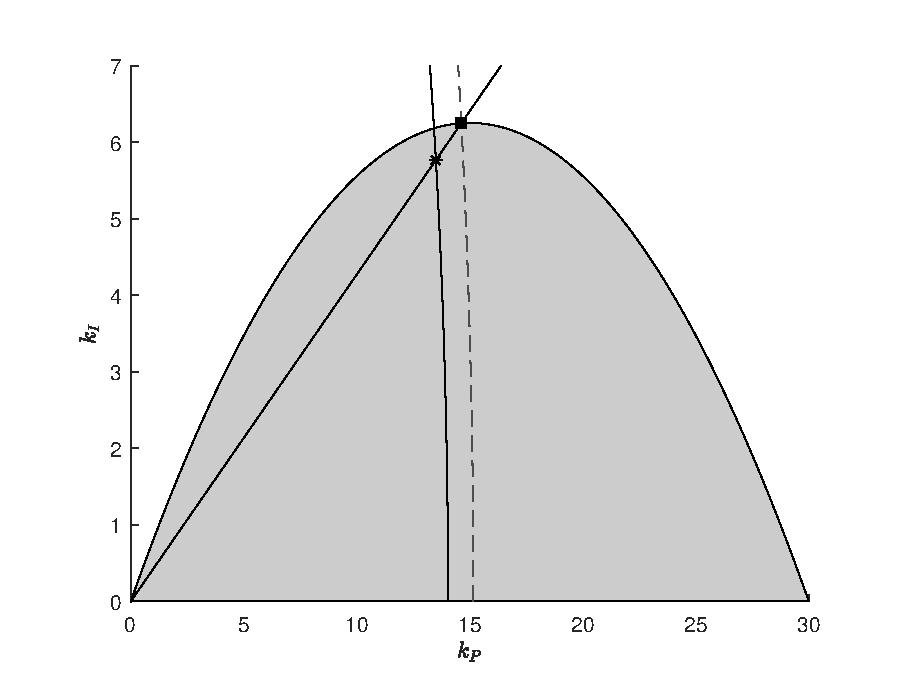
\includegraphics[width=0.5\textwidth]{Figs/curvas2-1}\label{curvas2a}}
	\subfigure[]{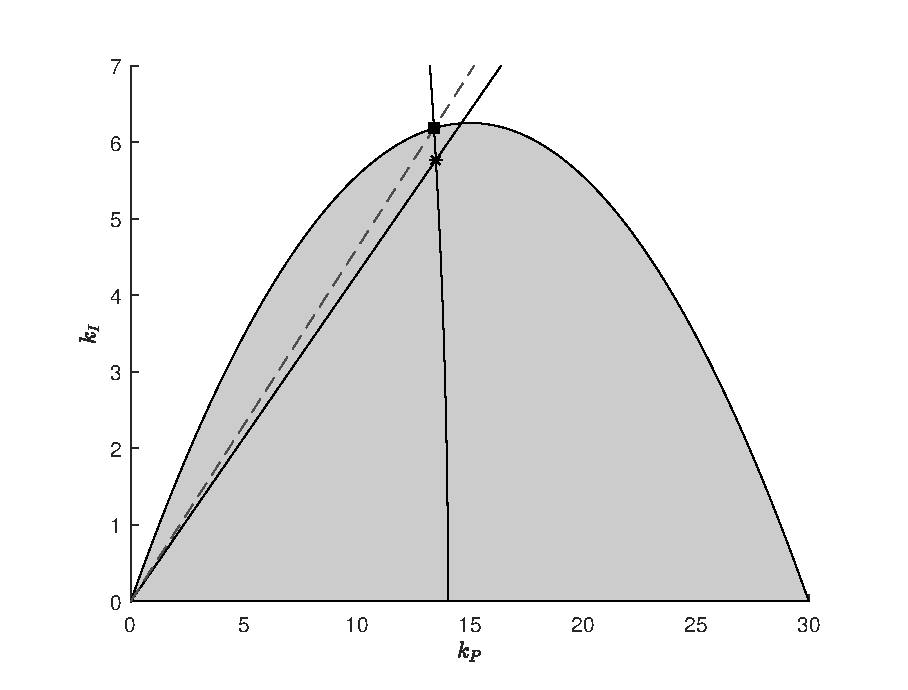
\includegraphics[width=0.5\textwidth]{Figs/curvas2-2}\label{curvas2b}}
\caption[Representaci�n en $\left(k_P, k_I \right)$ para m�rgenes de estabilidad]{Representaci�n geom�trica en el plano $\left(k_P, k_I \right)$ para m�rgenes de estabilidad: (a) $A_m$ manteniendo fija la recta y variando la elipse; (b) $\theta_m$ manteniendo fija la elipse y variando la recta}\label{curvas2}
\end{figure}
% ------------------------------------------------------------------------
\begin{figure}
\centering
	\subfigure[]{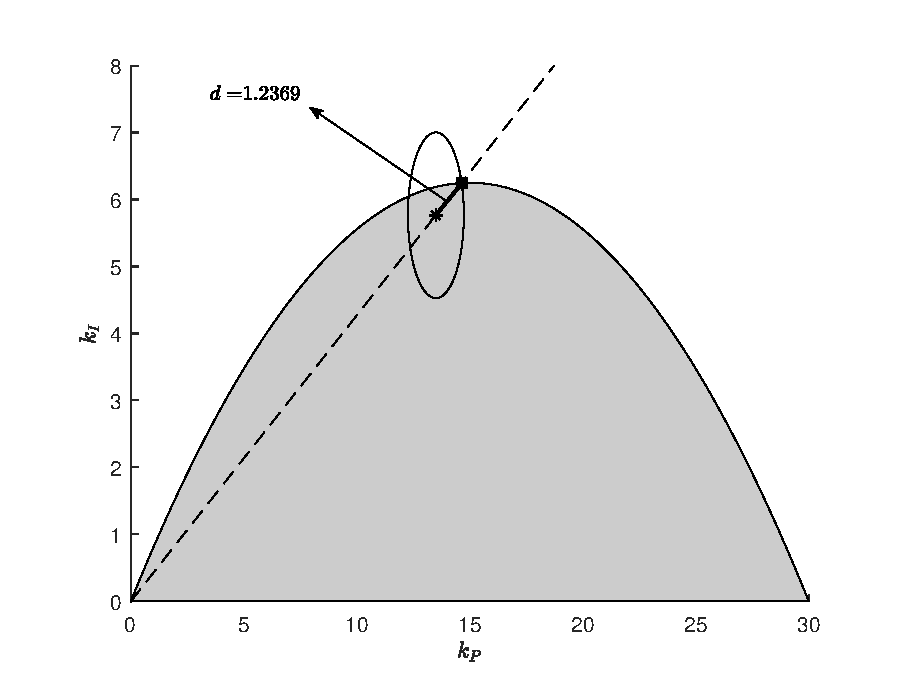
\includegraphics[width=0.5\textwidth]{Figs/max_dist_2}}
	\subfigure[]{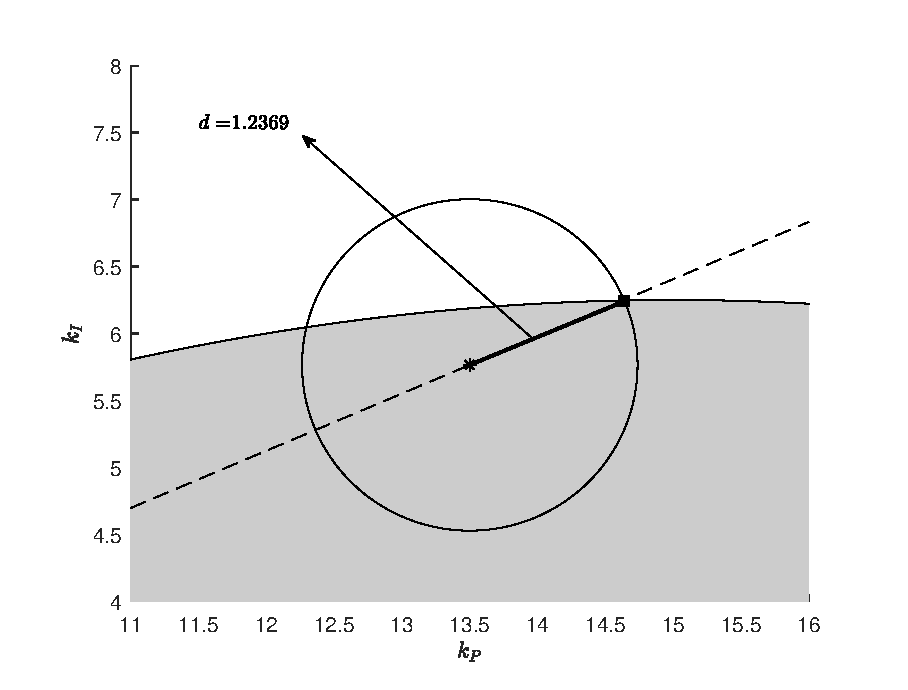
\includegraphics[width=0.5\textwidth]{Figs/max_dist}}
\caption[Distancia a la inestabilidad]{Distancia a la inestabilidad ilustrando: (a) panor�mica general de la m�trica y (b) detalle de la m�trica}\label{distancia}
\end{figure}
% ------------------------------------------------------------------------   % Controladores PI y su conjunto estabilizante
% ------------------------------------------------------------------------
% ------------------------------------------------------------------------
% ------------------------------------------------------------------------
%                            Recomendaciones
% ------------------------------------------------------------------------
% ------------------------------------------------------------------------
% ------------------------------------------------------------------------

\chapter{Recomendaciones}
% ------------------------------------------------------------------------
\noindent Al momento de ejecutar la interfaz desarrollada es importante que el usuario tenga una noci�n respecto al rango de valores que desea visualizar, pues esto hace m�s fino el detalle de los puntos sobre los cuales se calcula el conjunto estabilizante y por ende, la exploraci�n de los valores admisibles para el control en la pr�ctica.
% ------------------------------------------------------------------------    % Recomendaciones
% ------------------------------------------------------------------------
% ------------------------------------------------------------------------
% ------------------------------------------------------------------------
%                            Trabajo futuro
% ------------------------------------------------------------------------
% ------------------------------------------------------------------------
% ------------------------------------------------------------------------

\chapter{Trabajo futuro}
% ------------------------------------------------------------------------
\noindent Actividades complementarias a los desarrollos presentados, incluyen el c�lculo autom�tico para conjuntos estabilizantes en plantas arbitrarias empleando el \emph{m�todo de la signatura} desarrollado por Keel y Bhattacharyya en \citep{keel2008}.\\

Asimismo es importante explorar otras topologias de compensador y controladores PID, en sus versiones de tiempo continuo y discreto.
% ------------------------------------------------------------------------    % Trabajo futuro
% ------------------------------------------------------------------------
% ------------------------------------------------------------------------
% ------------------------------------------------------------------------
%                             Conclusiones
% ------------------------------------------------------------------------
% ------------------------------------------------------------------------
% ------------------------------------------------------------------------

\chapter{Conclusiones}
% ------------------------------------------------------------------------
% ------------------------------------------------------------------------
\noindent A partir de los desarrollos presentados y los resultados obtenidos en el presente trabajo de grado, es posible enunciar la siguiente conclusi�n general:\\
% ------------------------------------------------------------------------
\begin{itemize}
\item[ ] Se analizaron las condiciones de estabilidad del conjunto de par�metros PI calculados empleando el m�todo de dise�o de controladores de \emph{Ziegler \& Nichols}. Fue posible definir una m�trica para la inestabilidad del sistema controlado en el plano de par�metros $\left(k_P, k_I \right)$, a partir de una interpretaci�n geom�trica de los margenes de estabilidad del sistema. A partir de lo anterior fue posible valorar la \emph{fragilidad} del controlador PI dise�ado.\\
\end{itemize}
% ------------------------------------------------------------------------

De manera m�s puntual:\\
% ------------------------------------------------------------------------
\begin{itemize}
  \item[ ] Se interpretaron las tablas de dise�o de par�metros PI de \emph{Ziegler \& Nichols} en t�rminos de conjuntos estabilizantes. Tal y como fue abordado en la \emph{Secci�n} \ref{estabanalpi}, se ilustr� el dise�o de un compensador PI para una planta y posteriormente se analiz� la posici�n de dicho punto en el plano $\left(k_P, k_I \right)$ de controladores factibles con base en su conjunto estabilizante. A partir de ello, es claro que el m�todo de \emph{Ziegler \& Nichols} siempre dar� como resultado un controlador estable, tomando en cuenta su caracter emp�rico. Sin embargo, a partir de la definici�n de una m�trica en la \emph{Secci�n} \ref{metrdef}, fue posible mostrar a trav�s de una cuantificaci�n para su \emph{fragilidad} que no necesariamente el controlador calculado es estable ante ligeras variaciones en sus valores de par�metro. De otro lado, la definici�n de conjunto estabilizante fue ampliamente abordada en la \emph{Secci�n} \ref{conjestabsect} y posteriormente aplicada al caso PI en la \emph{Secci�n} \ref{estabanalpi}.
  \item[ ] Se desarroll� un algoritmo que permiti� verificar las condiciones de estabilidad para controladores PI dise�ados mediante el m�todo de \emph{Ziegler \& Nichols}. Inicialmente, se realiz� una discusi�n general de conjuntos estabilizantes en la \emph{Secci�n} \ref{conjestabsect}, posteriormente complementada en la \emph{Secci�n} \ref{conjestabpi} con medidas de inestabilidad a trav�s de una m�trica basada en la interpretaci�n geom�trica para m�rgenes de estabilidad en un lazo de control sometido a control PI. El m�todo (o algoritmo) consisti� fundamentalmente en calcular el conjunto estabilizante en el plano de par�metros del controlador, para posteriormente transformar las especificaciones de controladores viables a cantidades igualmente viables en el dominio del tiempo. Posteriormente un usario podr�a seleccionar el controlador deseado a partir de un punto en el conjunto de par�metros admisible, para el cual se provee adem�s indicaci�n de sus m�rgenes de estabilidad como medida de \emph{fragilidad}. El procedimiento anterior se desarroll� para los casos de un compensador de 3 par�metros (uno de ellos conocido) y un controlador PI.
  \item[ ] Se implement� una interfaz para c�lculo de controladores PI a partir de selecci�n de par�metros en el dominio del tiempo, admisibles respecto al conjunto estabilizante correspondiente. El algoritmo descrito en el �tem anterior fue codificado en una interfaz en MATLAB seg�n se describe en la \emph{Secci�n} \ref{interfazsect}, empleando una metodolog�a de dise�o del tipo \emph{top-down}.
\end{itemize}
% ------------------------------------------------------------------------    % Conclusiones
% ------------------------------------------------------------------------
% Bibliograf�a
% ------------------------------------------------------------------------
\addcontentsline{toc}{chapter}{Referencias Bibliogr�ficas}\newpage
\bibliographystyle{apalike}
\bibliography{xbib}
% ------------------------------------------------------------------------
% Anexos
% ------------------------------------------------------------------------
% ------------------------------------------------------------------------
% ------------------------------------------------------------------------
% ------------------------------------------------------------------------
%                                Anexo A
% ------------------------------------------------------------------------
% ------------------------------------------------------------------------
% ------------------------------------------------------------------------
% ------------------------------------------------------------------------
\newpage
\nnchapter{Ap�ndices}
% ------------------------------------------------------------------------
\anexo{Fundamentos de s�lidos r�gidos}\label{anexoA}
% ------------------------------------------------------------------------
\noindent Un s�lido r�gido, es un cuerpo formado por varias part�culas puntuales que
guardan distancias constantes entre s� \citep{sears2005fisica}.\\

Una operaci�n fundamental para definir cantidades en el espacio de movimiento de
un s�lido r�gido es el producto vectorial (tambi�n denominado producto cruz \citep{stanley1993algebra}),
el cual produce un vector perpendicular (normal) al plano formado por otros dos vectores
que se multiplican.\\

Sean dos vectores $\vec{a}$ y $\vec{b}$ definidos en $\mathbb{R}^3$. El producto vectorial entre $\vec{a}$ y $\vec{b}$ (denotado $\vec{a} \times \vec{b}$) es otro vector (digamos $\vec{c} \in \mathbb{R}^3$) cuyo c�lculo puede ser efectuado a trav�s de determinantes como sigue:
% ------------------------------------------------------------------------
\begin{equation}\label{defprodvect}
\vec{c} = \vec{a} \times \vec{b} = \begin{vmatrix}
i& j & k \\
a_i & a_j  & a_k \\
b_i & b_j  & b_k
\end{vmatrix} =
\begin{vmatrix}
 a_j & a_k \\
 b_j & b_k
\end{vmatrix}i~
-
\begin{vmatrix}
a_i & a_k \\
b_i & b_k
\end{vmatrix}j~
+\begin{vmatrix}
 a_i & a_j \\
 b_i & b_j
\end{vmatrix}k
\end{equation}
% ------------------------------------------------------------------------
De esta manera, siendo $\vec{a}=(1,-1,2)$ y $\vec{b}=(3,-4,5)$ se obtiene:
% ------------------------------------------------------------------------
\begin{equation}
\vec{a} \times \vec{b} =\begin{vmatrix}
i& j & k \\
1 &-1  &2 \\
3 &-4  &5
\end{vmatrix}=
\begin{vmatrix}
 -1&2 \\
 -4&5
\end{vmatrix}i~
-
\begin{vmatrix}
1 &2 \\
3 &5
\end{vmatrix}j~
+\begin{vmatrix}
 1&-1 \\
 3&4
\end{vmatrix}k
= 3i-j-k
\end{equation}
% ------------------------------------------------------------------------
La Fig. \ref{prodvect} ilustra esta operaci�n gr�ficamente en el espacio tridimensional.
% ------------------------------------------------------------------------
\begin{figure}[h]
\centering
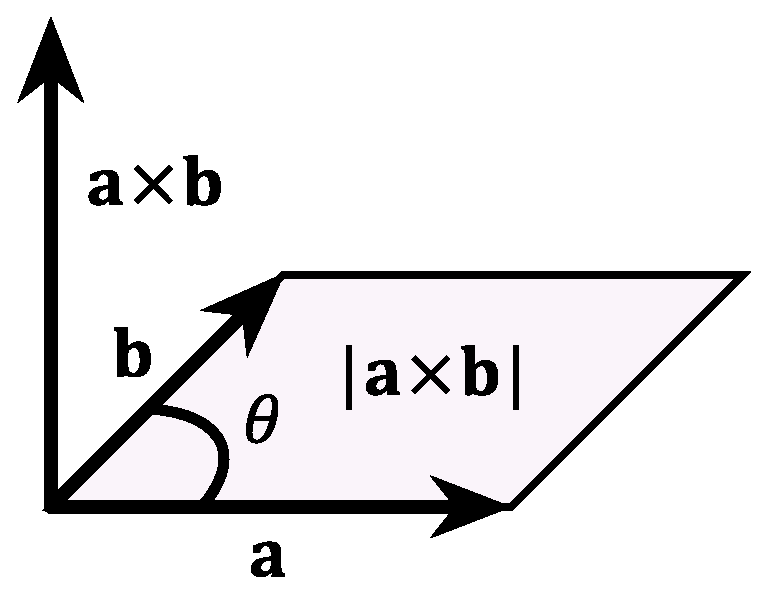
\includegraphics[width=0.3\textwidth]{Figs/prodvect}
\caption[]{Ilustraci�n gr�fica para producto vectorial}\label{prodvect}
\end{figure}
% ------------------------------------------------------------------------

\section*{Condici�n de rigidez}
% ------------------------------------------------------------------------
\noindent Considere el s�lido r�gido presentado en la Fig. \ref{rigid}. Para cada pareja de puntos $(P_i, P_j)$ pertenecientes al s�lido, se cumple:
% ------------------------------------------------------------------------
\begin{equation}\label{rigidez}
\frac{d}{dt}[\left|r_i - r_j\right|] = \frac{d}{dt}[\left|r_{ij}\right|] = 0,
\end{equation}
% ------------------------------------------------------------------------
lo cual significa que la distancia entre puntos de un s�lido r�gido se mantiene invariante. Esto �ltimo se conoce como la \emph{condici�n de r�gidez}.\\
% ------------------------------------------------------------------------
\begin{figure}[h]
\centering
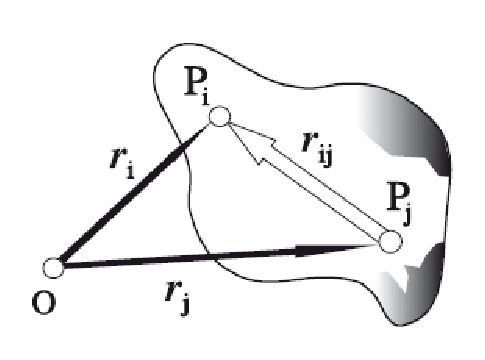
\includegraphics[width=0.3\textwidth]{Figs/rigid}
\caption[]{S�lido r�gido}\label{rigid}
\end{figure}
% ------------------------------------------------------------------------

Asimismo, a partir de \eqref{rigidez} se obtiene:
% ------------------------------------------------------------------------
\begin{equation}
\frac{d}{dt}[\left|r_i - r_j\right|] = \left|\dot{r}_i - \dot{r}_j\right| = 0,
\end{equation}
% ------------------------------------------------------------------------
y por tanto, sabiendo que $\vec{\dot{r}}$ es el vector velocidad $\vec{v}$ para un punto del s�lido visto desde el observador, es posible escribir:
% ------------------------------------------------------------------------
\begin{equation}
\left|v_i\right| = \left|v_j\right|,
\end{equation}
% ------------------------------------------------------------------------
con lo cual la velocidad de traslaci�n para cualquier punto del s�lido ser� la misma, y as�, una vez definido el movimiento de un punto cualquiera del cuerpo rigido que se traslada en el espacio, es posible definir la totalidad de su movimiento.

% ------------------------------------------------------------------------
\section*{Movimiento de rotaci�n}
% ------------------------------------------------------------------------
\noindent En la Fig. \ref{rotacion} se ilustra un punto que rota alrededor de un eje fijo, localizado en el cuerpo del s�lido.\\
% ------------------------------------------------------------------------
\begin{figure}[h]
\centering
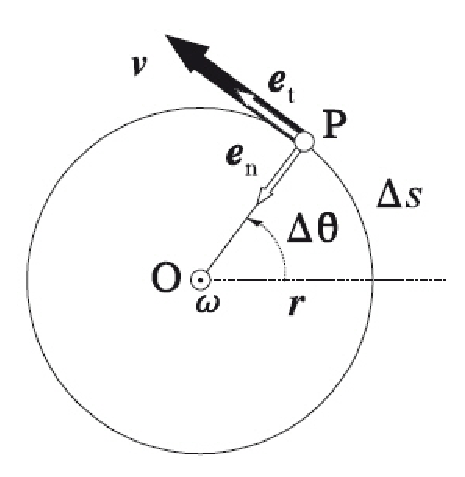
\includegraphics[width=0.3\textwidth]{Figs/rotacion}
\caption[]{Rotaci�n de un punto del s�lido alrededor de un eje fijo}\label{rotacion}
\end{figure}
% ------------------------------------------------------------------------

A partir de ello, es posible definir la velocidad angular que experimenta el punto $P$ alrededor del eje de rotaci�n, en el modo siguiente:
% ------------------------------------------------------------------------
\begin{equation}
\omega = \frac{d}{dt}\theta
\end{equation}\
% ------------------------------------------------------------------------

Tambien, puede escribirse del diagrama la velocidad tangencial $v$ del punto mediante:
% ------------------------------------------------------------------------
\begin{equation}
\vec{v} = \vec{r} \times \vec{\omega},
\end{equation}
% ------------------------------------------------------------------------
siendo $\vec{r}$ el vector que marca la distancia del punto $P$ al eje de rotaci�n $O$.\\

Por tanto, el vector de aceleraci�n puede ser formulado como:
% ------------------------------------------------------------------------
\begin{eqnarray}\label{aceler}
\nonumber \frac{d}{dt}\vec{v} & = & \frac{d}{dt}[\vec{r} \times \vec{\omega}]\\
\nonumber & = & \left( \frac{d}{dt}\vec{r}\times \vec{\omega}\right) + \left( \vec{r}\times \frac{d}{dt}\vec{\omega}\right)\\
\vec{a}   & = & \vec{r} \times \vec{\alpha},
\end{eqnarray}
% ------------------------------------------------------------------------
con $\vec{a}$ y $\vec{\alpha}$ representando, respectivamente, los vectores de aceleraci�n lineal y angular. Note que se asume $\frac{d}{dt}\vec{r} = 0$ debido a que el eje de rotaci�n es fijo.

% ------------------------------------------------------------------------
\section*{Conservaci�n del momento angular}
% ------------------------------------------------------------------------
\noindent En un movimiento traslacional, el principio de conservaci�n del momento lineal establece:
% ------------------------------------------------------------------------
\begin{equation}
\frac{d}{dt}\vec{p} = \frac{d}{dt}{m\vec{v}} = 0,
\end{equation}
% ------------------------------------------------------------------------
a partir de lo cual el momento $\vec{p}$ ser� constante en ausencia de fuerzas externas.\\

De manera similar, es posible definir el momento angular $\vec{\mathbf{L}}$ de una part�cula de masa puntual que rota alrededor de un eje fijo, en el modo siguiente:
% ------------------------------------------------------------------------
\begin{equation}\label{momang}
\vec{\mathbf{L}} = \vec{r} \times \vec{p},
\end{equation}
% ------------------------------------------------------------------------
siendo $\vec{r}$ el vector de distancia a la masa desde el centro de rotaci�n.\\

Por tanto, el principio de conservaci�n del momento angular puede establecerse como sigue:
% ------------------------------------------------------------------------
\begin{eqnarray*}
\frac{d}{dt}\vec{\mathbf{L}} & = & \frac{d}{dt}{[\vec{r} \times \vec{p}]} \\
                             & = & \frac{d}{dt}{[\vec{r} \times m\vec{v}]}\\
                             & = & m \frac{d}{dt}{[\vec{r} \times \vec{v}]}\\
                             & = & m\left([\vec{r}\times\frac{d}{dt}\vec{v}]+[\frac{d}{dt}\vec{r}\times\vec{v}]\right)\\
                             & = & m\left([\vec{r}\times \vec{a}]+[\vec{v}\times\vec{v}]\right)\\
                             & = & \vec{r}\times m\vec{a}\\
                             & = & \vec{r}\times \vec{F}\\
                             & = & \tau,
\end{eqnarray*}
% ------------------------------------------------------------------------
siendo $\tau$ el torque neto aplicado.\\

Empleando \eqref{aceler} puede relacionarse este torque con la aceleraci�n angular $\vec{\alpha}$, a partir de:
% ------------------------------------------------------------------------
\begin{eqnarray*}
\tau & = & \vec{r}\times m\vec{a}\\
     & = & \vec{r}\times m\left(\vec{r} \times \vec{\alpha}\right)\\
     & = & m\left(\vec{r}\times \left(\vec{r} \times \vec{\alpha}\right)\right)
\end{eqnarray*}
% ------------------------------------------------------------------------
donde, si $\vec{r}$ es perpendicular a $\vec{\alpha}$, entonces el producto vectorial se reduce al producto de las magnitudes:
% ------------------------------------------------------------------------
\begin{eqnarray}\label{newrot}
\nonumber \tau & = & m r^2 \alpha \\
               & = & I \alpha,
\end{eqnarray}
% ------------------------------------------------------------------------
siendo $I$ el momento de inercia de las partes rotativas del cuerpo r�gido.\\

La expresi�n \eqref{newrot} es la segunda ley de Newton de rotaci�n, y podr� ser definida siempre que sea v�lido un $I$ constante. Dicha situaci�n no siempre es posible, principalmente si se asume que el eje de rotaci�n puede variar en el tiempo. En tal caso, $\vec{r}$ en la Fig. \ref{rotacion} no es constante y por tanto no es v�lida la soluci�n propuesta para $\vec{a}$ en \eqref{aceler}, resultando en la siguiente definici�n alternativa para $\tau$:
% ------------------------------------------------------------------------
\begin{eqnarray*}
\tau & = & \vec{r}\times m\vec{a}\\
     & = & \vec{r}\times m\left(\left( \frac{d}{dt}\vec{r}\times \vec{\omega}\right) + \left( \vec{r}\times \frac{d}{dt}\vec{\omega}\right)\right)\\
     & = & m\left(\left[\vec{r}\times\left( \frac{d}{dt}\vec{r}\times \vec{\omega}\right)\right] + \left[\vec{r}\times\left( \vec{r}\times \vec{\alpha}\right)\right]\right)\\
     & = & m\left(\left[\vec{r}\times\left( \frac{d}{dt}\vec{r}\times \vec{\omega}\right)\right]\right) + I\alpha.
\end{eqnarray*}\
% ------------------------------------------------------------------------

El t�rmino
% ------------------------------------------------------------------------
$$
m\left(\left[\vec{r}\times\left( \frac{d}{dt}\vec{r}\times \vec{\omega}\right)\right]\right),
$$\
% ------------------------------------------------------------------------
representa los efectos (torques) debidos a las variaciones del eje de rotaci�n, que evidentemente tambi�n representan variaciones del vector de momento angular $\vec{\mathbf{L}}$. Dichos efectos se denominan \emph{fuerzas inerciales}, puesto que tienen sentido en un marco de referencia de un cuerpo en rotaci�n. Los tipos m�s representativos de fuerza inercial son los efectos girosc�picos y la fuerza de Coriollis \citep{sears2005fisica}.
% ------------------------------------------------------------------------  % Fundamentos de s�lidos r�gidos
% ------------------------------------------------------------------------
% ------------------------------------------------------------------------
% ------------------------------------------------------------------------
%                                Anexo B
% ------------------------------------------------------------------------
% ------------------------------------------------------------------------
% ------------------------------------------------------------------------
% ------------------------------------------------------------------------
\newpage
\anexo{Funci�n \emph{ode45} de MATLAB}\label{anexoB}
% ------------------------------------------------------------------------
\noindent La funci�n $ode45$ est� basada en un algoritmo de tipo Runge-Kutta, que se desarroll� a partir del m�todo de Euler mejorado \citep{chapra2003metodos}. La funci�n recibe tres par�metros esenciales: $f(t)$ dentro de un $script$ en el que se define la ecuaci�n diferencial acompa�ado por un simbolo $@$, el vector de l�mites de tiempo $\left[ t_0 \quad t_f \right]$ y el vector de condiciones iniciales $y_0$. En otras palabras el prototipo b�sico para usar \emph{ode45} es el siguiente:
% ------------------------------------------------------------------------
\begin{equation}\label{defode}
   [t,y]=\emph{ode45}(@f(t),\left[ t_0 \quad t_f \right],y_0);
    \end{equation}
% ------------------------------------------------------------------------
En este caso la soluci�n num�rica se almacenar� en el vector $y$  para cada uno de los instantes de tiempo presentes en el vector $t$.\\

La funci�n $ode45$, resuelve ecuaciones del tipo $\dot{y} = f(t,y)$, por tanto si se desea resolver ecuaciones de orden superior estas deben escribirse como un sistema de ecuaciones diferenciales de primer orden.\\

A manera de ejemplo, se ilustrar� la forma de resolver la ecuaci�n diferencial de segundo orden
% ------------------------------------------------------------------------
\begin{equation}\label{segundo}
   \ddot{x}-\mu\left(1-x^2\right)\dot{x}+x=0,
\end{equation}
% ------------------------------------------------------------------------
donde $\mu > 0$ es un par�metro escalar.\\

Por tanto, definiendo
% ------------------------------------------------------------------------
$$y_1 = x; \quad y_2 = \dot{x}$$
% ------------------------------------------------------------------------
la expresi�n \eqref{segundo} puede ser reescrita como
% ------------------------------------------------------------------------
$$
\dot{y}_2 = \mu \left( 1 - y_1^2 \right) y_2 + y_1
$$
% ------------------------------------------------------------------------
es decir, transformando la ecuaci�n diferencial original de segundo orden y una variable, en una ecuaci�n diferencial equivalente de primer orden y dos variables. As� entonces, es posible construir el vector
% ------------------------------------------------------------------------
$$
y = \left[ {\begin{array}{*{20}c}
   y_1  \\
   y_2  \\
\end{array}} \right]
$$
% ------------------------------------------------------------------------
cuya din�mica viene representada por
% ------------------------------------------------------------------------
$$
\dot{y} = \left[ {\begin{array}{*{20}c}
   f_1 \left(t, y \right)  \\
   f_2 \left(t, y \right) \\
\end{array}} \right]
$$
% ------------------------------------------------------------------------
siendo
% ------------------------------------------------------------------------
$$f_1\left(t, y \right) = y_2; \quad f_2\left(t, y \right) =  \mu \left( 1 - y_1^2 \right) y_2 + y_1$$
% ------------------------------------------------------------------------
De esta manera, evaluar la expresi�n \eqref{defode} permite obtener una matriz de salida $y$ con filas representando los vectores soluci�n para $y_1$ e $y_2$ como funci�n de $t$.\\
% ------------------------------------------------------------------------

\begin{figure}[h]
\centering
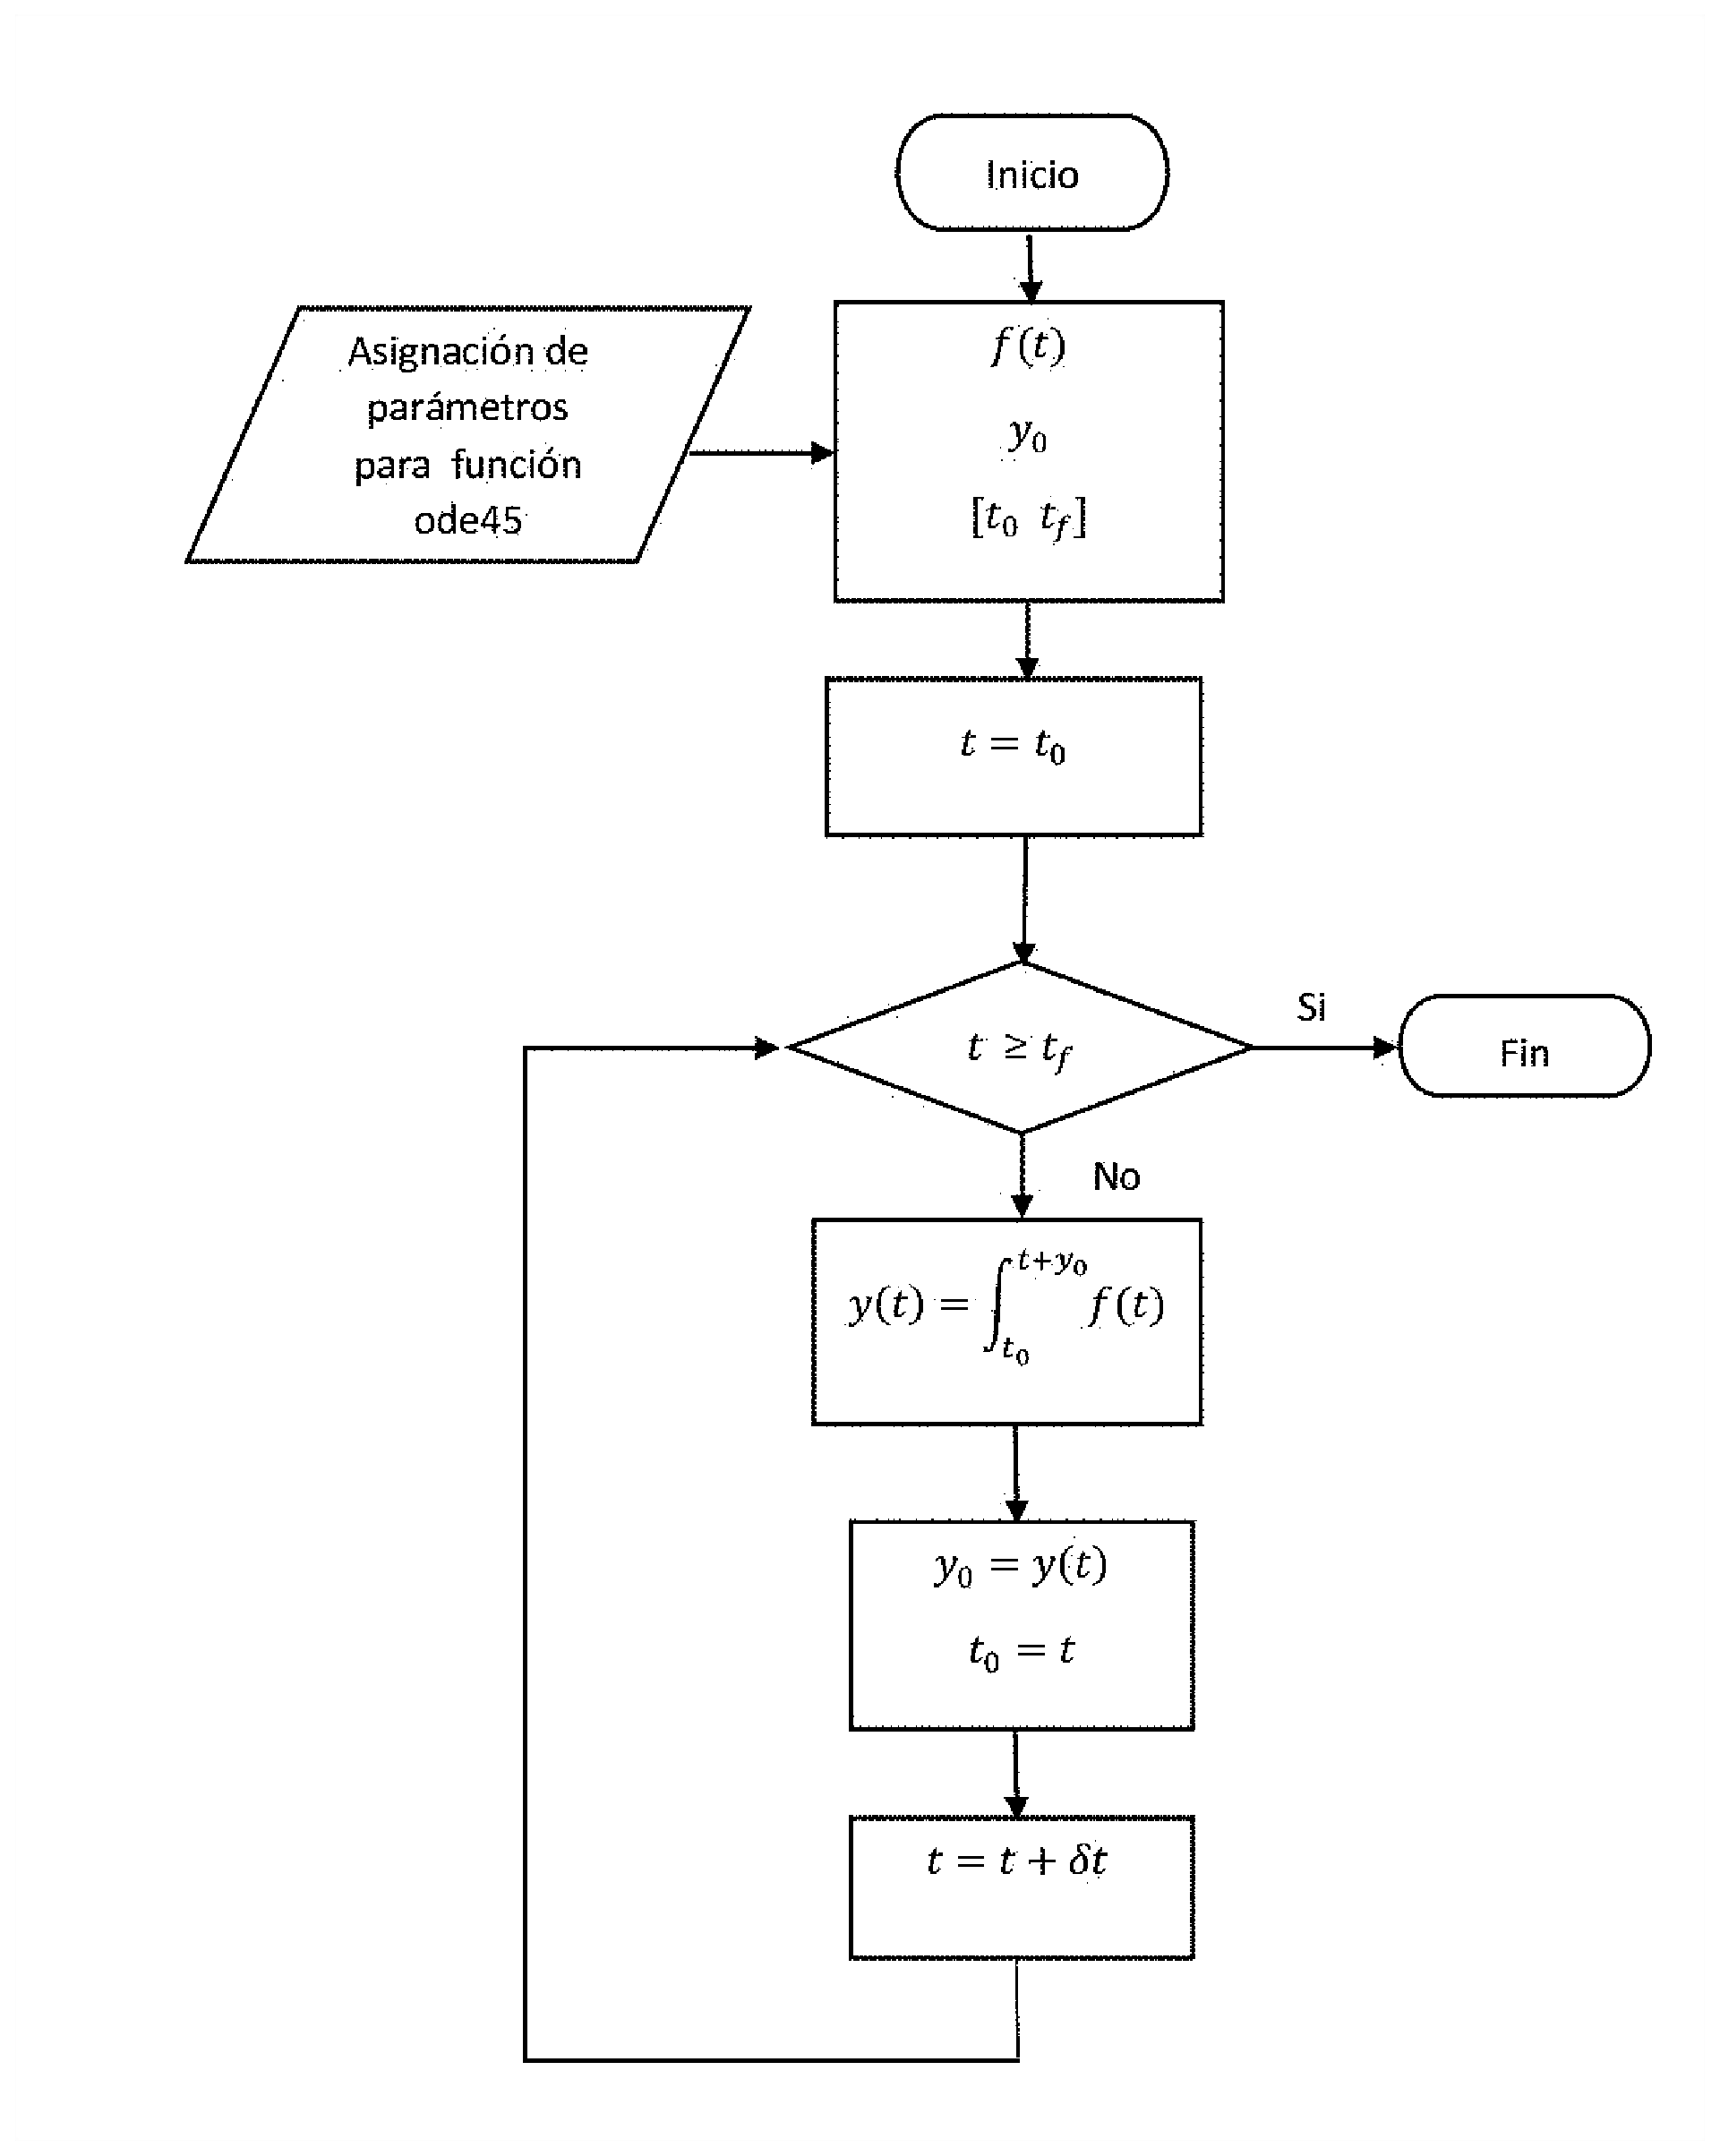
\includegraphics[width=0.55\textwidth]{Figs/flujodiag}
\caption[]{Diagrama de flujo para algoritmo de integraci�n num�rica de la funci�n $ode45$ de MATLAB}\label{flujodiag}
\end{figure}
% ------------------------------------------------------------------------

En la Fig. \ref {flujodiag} se ilustra el diagrama de flujo del algoritmo empleado para hallar la soluci�n de una ecuaci�n diferencial mediante integraci�n num�rica empleando la funci�n $ode45$ de MATLAB.\\

Inicialmente, se deben asignar los par�metros definidos en la ecuaci�n \eqref{defode}.\\

Posteriormente, un bucle interno hace llamado iterativo a la funci�n $f(t)$ evaluada para valores de tiempo entre $t_0$ y $t_f$ a partir de las condiciones iniciales $y_0$. Para cada ciclo la condici�n inicial se recalcula siendo la condici�n final del ciclo anterior. El tiempo se incrementa en un tama�o de paso $\delta t$ de forma adaptativa, si no se especifica lo contrario. Tras alcanzarse el tiempo final $t_f$, el bucle interno termina y entrega como resultado el vector de puntos de la trayectoria soluci�n $y(t)$ al igual que el vector de tiempos $t$.  % Funci�n ode45 de MATLAB
% ------------------------------------------------------------------------
% ------------------------------------------------------------------------
% ------------------------------------------------------------------------
%                                Anexo C
% ------------------------------------------------------------------------
% ------------------------------------------------------------------------
% ------------------------------------------------------------------------
% ------------------------------------------------------------------------
\newpage
\anexo{Interfaz de animaci�n de la din�mica del sistema}\label{anexoC}
% ------------------------------------------------------------------------
\noindent En ausencia de un prototipo real para verificar el comportamiento din�mico del sistema controlado, se opt� por construir una animaci�n que permitiera recrear el movimiento del \emph{dron} de una manera cercana al comportamiento f�sico real. A continuaci�n se presentan las etapas importantes para este desarrollo.

% ------------------------------------------------------------------------
\section*{Descripci�n general de requerimientos}
% ------------------------------------------------------------------------
\noindent Se requiere construir una interfaz de software que permita visualizar el comportamiento del dron en el espacio de movimiento, como aproximaci�n a la operaci�n real del sistema para diferentes condiciones de simulaci�n (lazo abierto, lazo cerrado controlado PID y por realimentaci�n de estados) ante la presencia de perturbaciones. La interfaz deber� permitir modificar par�metros del sistema y los par�metros de simulaci�n, as� como tambi�n entregar informaci�n de las trayectorias de variables con respecto al tiempo.

% ------------------------------------------------------------------------
\subsection*{Nivel superior de detalle}
% ------------------------------------------------------------------------
\noindent Posterior a tener una descripci�n, en palabras, acerca de los requerimientos del sistema (interfaz) a desarrollar, el paso siguiente es crear un diagrama general de entradas y salidas a manera de nivel superior de detalle. Dicho diagrama se presenta en la Fig. \ref{1211}.
% ------------------------------------------------------------------------
\begin{figure}[h]
\centering
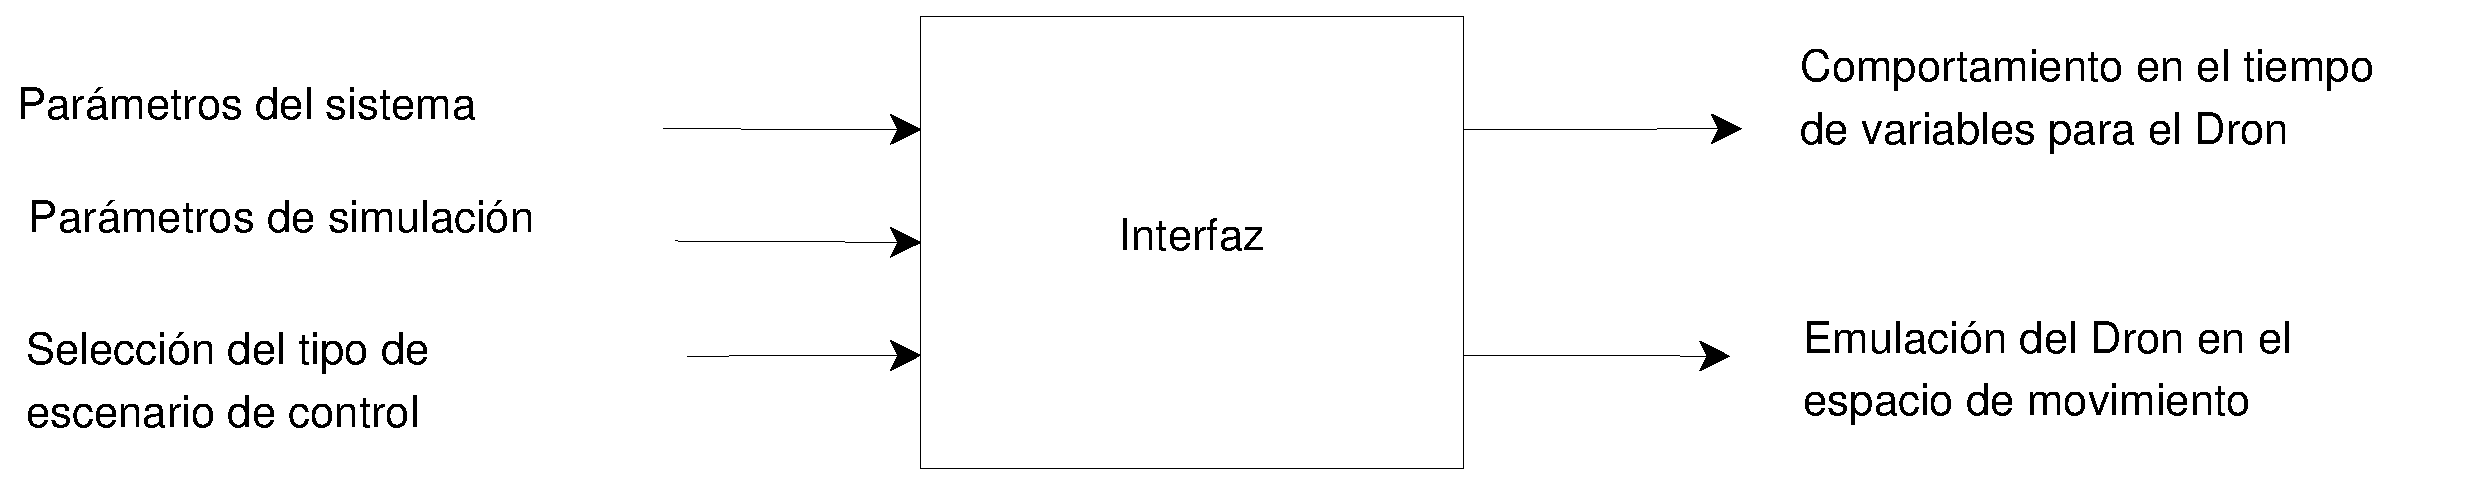
\includegraphics[width=0.7\textwidth]{figs/primero}
\caption[]{Representaci�n de nivel superior de detalle para desarrollo de interfaz}\label{1211}
\end{figure}

% ------------------------------------------------------------------------
\subsection*{Partici�n de primer nivel}
% ------------------------------------------------------------------------
\noindent Una primera partici�n se logra incorporando el bloque que realiza la soluci�n num�rica de las ecuaciones del sistema, a partir de los par�metros de entrada en el modelo y los valores que configuran la simulaci�n, seg�n se muestra en la Fig. \ref{1212}.\\
% ------------------------------------------------------------------------
\begin{figure}
\centering
\includegraphics[width=0.7\textwidth]{figs/segunda}
\caption[]{Representaci�n de primer nivel de partici�n para subproceso de simulaci�n}\label{1212}
\end{figure}

% ------------------------------------------------------------------------
Asimismo, los resultados de este simulador ser�n la entrada de un nuevo bloque encargado de construir una animaci�n para emular el comportamiento del \emph{dron} en el espacio de movimiento. Una ilustraci�n para este segundo bloque se presenta en la Fig. \ref{1213} donde se observa tambi�n que ser� necesario configurar algunas opciones de simulaci�n incorporadas como se�al de entrada.\\
% ------------------------------------------------------------------------
\begin{figure}
\centering
\includegraphics[width=0.7\textwidth]{figs/tercero}
\caption[]{Representaci�n de primer nivel de partici�n para subproceso de animaci�n}\label{1213}
\end{figure}
% ------------------------------------------------------------------------

Finalmente, este primer nivel de partici�n se completa uniendo los dos subprocesos tal y como se ilustra en la Fig. \ref{1214}.
% ------------------------------------------------------------------------
\begin{figure}
\centering
\includegraphics[width=0.7\textwidth]{figs/cuarta}
\caption[]{Representaci�n de primer nivel de partici�n para desarrollo de interfaz}\label{1214}
\end{figure}

% ------------------------------------------------------------------------
\subsubsection*{Partici�n de segundo nivel}
% ------------------------------------------------------------------------
\noindent A su vez, es posible abrir el bloque correspondiente a la simulaci�n de las ecuaciones del sistema (seg�n se observa en la Fig. \ref{16}) para permitir incorporar la selecci�n del escenario de control que define una configuraci�n importante como lo es la forzante de entrada $\Delta\boldsymbol\tau(t)$ en el modelo. De manera similar, el bloque que realiza la soluci�n en el tiempo para las ecuaciones del sistema es un integrador num�rico.\\
% ------------------------------------------------------------------------
\begin{figure}
\centering
\includegraphics[width=0.7\textwidth]{figs/quinto}
\caption[]{Representaci�n de segundo nivel de partici�n para subproceso de simulaci�n}\label{16}
\end{figure}

% ------------------------------------------------------------------------
Por tanto, en la Fig. \ref{1515} se muestra el diagrama de bloques resultante para este segundo y definitivo nivel de detalle.
% ------------------------------------------------------------------------
\begin{figure}
\centering
\includegraphics[width=0.9\textwidth]{figs/sexto}
\caption[]{Diagrama de interconexi�n de susbsistemas que conforman la interfaz de animaci�n de la planta}\label{1515}
\end{figure}

% ------------------------------------------------------------------------
\subsection*{Selecci�n de herramienta para implementaci�n}
% ------------------------------------------------------------------------
\noindent A partir del diagrama obtenido en la Fig. \ref{1515}, es claro que el coraz�n de la interfaz a ser dise�ada es el integrador num�rico que resuelve las ecuaciones del sistema. Como ya ilustrado en el Anexo \ref{anexoB}, este integrador num�rico ha sido codificado empleando la funci�n $ode45$ de MATLAB. Por tanto, con el objetivo de facilitar la utilizaci�n de los desarrollos num�ricos a disposici�n, se presenta a MATLAB como la primera opci�n para desarrollar la herramienta de software requerida.\\

Ahora bien, el segundo elemento importante de la interfaz es la animaci�n que permite emular el comportamiento del \emph{dron} en el espacio de movimiento. Por tanto, aunque no es restricci�n que ambas componentes de la interfaz (simulador y bloque de animaci�n) sean desarrollados en el mismo lenguaje de programaci�n, s� se considera conveniente esta opci�n por motivos ligados principalmente a la reducci�n en tiempos de desarrollo y a una mayor compatibilidad entre componentes.\\

Adicional a esto, se recuerda que MATLAB posee adem�s de la consola de comandos y el entorno de programaci�n gr�fico SIMULINK, un entorno para el desarrollo de interfaces de usuario denominado GUIDE (Graphical User Interface Development Environment).\\

Tomando en consideraci�n todo lo anterior, se selecciona MATLAB \emph{vR2014a} para construir la interfaz de usuario que satisface los requerimientos de dise�o ilustrados en el diagrama de nivel de partici�n presentado en la Fig. \ref{1515}.

% ------------------------------------------------------------------------
\subsection*{Descripci�n de interfaz dise�ada}
% ------------------------------------------------------------------------
\begin{figure}
\centering
\includegraphics[width=0.7\textwidth]{figs/interfaz}
\caption[]{Presentaci�n final para interfaz desarrollada}\label{siete}
\end{figure}

% ------------------------------------------------------------------------
\noindent Procediendo con el dise�o, se realiza codificaci�n en MATLAB para el diagrama de bloques de la Fig. \ref{1515}, asumiendo las siguientes variables de entrada:
% ------------------------------------------------------------------------
\begin{itemize}
    \item Par�metros de la planta: [$g$, $m$, $l$, $k_\tau$, $b$, $J_G$, $I_{xx}$, $I_{yy}$, $I_{zz}$, $A_z$];
    \item Selecci�n del tipo de escenario de control: [lazo abierto, lazo cerrado, PID, regulado espacio de estados, seguimiento espacio de estados];
    \item Par�metros de simulaci�n: [tiempo de simulaci�n, tiempo de perturbaci�n, amplitud de perturbaci�n],
\end{itemize}
% ------------------------------------------------------------------------
y de salida:
% ------------------------------------------------------------------------
\begin{itemize}
 \item Comportamiento en el tiempo de variables para sistema \emph{dron}: [posici�n en eje $z$; �ngulos de balanceo $\phi$, cabeceo $\theta$ y gui�ada $\psi$; vector de velocidades de traslaci�n $\mathbf{v}$; vector de velocidades angulares $\mathbf{\eta}$; vector de forzantes de control $\Delta\boldsymbol\tau$].
\end{itemize}\
% ------------------------------------------------------------------------
Asimismo, se requieren los comandos de control de interfaz siguientes:
% ------------------------------------------------------------------------
\begin{itemize}
 \item Reset: para reiniciar las variables del programa;
 \item Tipo de visualizaci�n: para seleccionar el gr�fico de salida a visualizar;
 \item Simular: para llamar el inicio de una simulaci�n;
 \item Salida: para terminar el programa.
\end{itemize}\
% ------------------------------------------------------------------------
Todo lo anterior fue adecuado como se presenta en la Fig. \ref{siete}, ilustrando la presentaci�n final de la interfaz desarrollada.
% ------------------------------------------------------------------------  % Interfaz de animaci�n de la din�mica del sistema
% ------------------------------------------------------------------------
\end{document}                                          % Fin de documento
% ------------------------------------------------------------------------ 